%!TEX root = ../template.tex
%%%%%%%%%%%%%%%%%%%%%%%%%%%%%%%%%%%%%%%%%%%%%%%%%%%%%%%%%%%%%%%%%%%%
%% chapter5.tex
%% NOVA thesis document file
%%
%% Chapter with Results 
%% Use case study
%% Tests Realized
%% My part is in this part of the data
%%%%%%%%%%%%%%%%%%%%%%%%%%%%%%%%%%%%%%%%%%%%%%%%%%%%%%%%%%%%%%%%%%%%

%%%%%%%%%%%%%%%%%%%%%%%  Start Results  %%%%%%%%%%%%%%%%%%%%%%%%%%%%%%%%

\chapter{Results}
\label{cha:Results}
This chapter will cover the results of the system.  It will start by explaining the used Methodology, followed by the presentation of the use cases where this thesis is integrated.
Then the geolocation, communication resilience and power results, are presented to the reader, concluding with the a comparison, and a discussion of the obtained results.

%%%%%%%%%%%%%%%%%%%%%%  Start Methodology %%%%%%%%%%%%%%%%%%%%%%%%%%%%%%

\section{Methodology}
\label{sec:methodology}
%%%PAPER
%%%<Describe shortly HOW you did address the problem. List a few of key existing scientific/technical achievements/solutions/theories/surveys you will rely upon in addressing the problem.>
%%%

To respond to the  presented  research question, this work explains the development of an Adaptive Geolocation Solver model, capable of autonomously decide the best location method. To reach a model able of the mentioned autonomous feature, it must address distinct variables as remaining battery and the availability of communication technologies. This availability can be analyzed through advanced sensing of the surrounding radio signals. This means that the model has to be aware of the environment in which the device is working. The environment main characteristic relates to indoor or outdoor and rural or urban. 
These characteristics have a direct impact on what kind of technology, has to be used in each working moment for each environment. Thus, the final idea is to define a model that responds to all of these situations, and consequently develop a correspondent profile-based decision system capable to respond to each situation.


For the development of the profile-based decision system, tests were conducted into two different environments urban and rural. Thus these tests used geolocation technologies such as GNSS, Wi-Fi and LoRa.
Furthermore, these tests will consist of the gathering information from different location coordinates, at different speeds as well as stationary, to evaluate the performance of the different technologies against each other. 

In addition, these tests were integrated into the Carelink project. It was used a geo-fencing polygon, previously defined by the carer of the~\gls{PwD} in the Carelink platform. Consequently, the device communicates with the platform to give its position and receive support on the technologies to use accordingly to the profiles of the respective~\gls{PwD}. Thus, in the end, these tests were conducted with real patients in real life trials. To perform this communication between the devices and the Carelink platform it was utilised LoRa and NB-IoT.


%%%%%%%%%%%%%%%%%%%%  Section Methodology (end) %%%%%%%%%%%%%%%%%%%%

%%%%%%%%%%%%%%%%%%%%%%  Section Material %%%%%%%%%%%%%%%%%%%%%%%%%%%%%%
\subsection{Material}
\label{subsec:material}
In order to conduct the tests of this work, it was selected $5$ FiPy devices, used in the belt  box format. That were used by the participants. 
The remaining material needed was a LoRa Gateway to ensure the coverage of LoRa signal, and a laptop to analyse the data.

%%%%%%%%%%%%%%%%%%%%%%%%%  Section Material (end) %%%%%%%%%%%%%%%%%%%%%%%%%%

%%%%%%%%%%%%%%%%%%%%%%%%%  Section Participants %%%%%%%%%%%%%%%%%%%%%%%%%%%
\subsection{Participants}
\label{subsec:Participants}
The participants in this experiment were $6$, later in this chapter will describe three different environments, where the tests took place. The participant for the first environment is male 24 and does not have dementia. In the second environment, the first tests were conducted by two participants both male one with 24 other with 60 both without dementia. When these tests were concluded, the final ones were conducted with $4$ persons with dementia, $n$ male $n$ female with ages from $n$ to $n$.

%%%%%%%%%%%%%%%%%%%%%  Section Participants (end) %%%%%%%%%%%%%%%%%%%%%%%%%%

%%%%%%%%%%%%%%%%%%%%%  Section Procedure  %%%%%%%%%%%%%%%%%%%%%%%%%%%%%%%%%%
\subsection{Procedure}
\label{subsec:Procedure}
The adopted procedure for this work, during the development phase, was first used a FiPy and each location method was tested individually, and then each communication method, later this was all combined. In the Real People with dementia test phase, was given one device to each participant to use during the day. The data from these tests were then analysed by the author.
%%%%%%%%%%%%%%%%%%%%%%%  Section Procedure (end) %%%%%%%%%%%%%%%%%%%%%%%%%%%

%%%%%%%%%%%%%%%%%%%%%%%%%  Section Use cases %%%%%%%%%%%%%%%%%%%%%%%%%%%%%%
\section{Use Cases}

In this section will be described the different use cases for this thesis. The three  use cases are~\nameref{subsec:laboratory},~\nameref{subsec:real_world} and~\nameref{subsec:Use_case_Swiss}. In these use cases the objective was to get the results for the geolocation. 
For these objective  tests were conducted for the geolocation technologies both GNSS, and GNSS-free. These tests consisted of gathering information from different location points, at different speeds, to discover the geolocation accuracy of such technologies. 


%%%%%%%%%%%%%%%%%%%%%%%%  Start use case 1  %%%%%%%%%%%%%%%%%%%%%%%%%%%%
\newpage

\subsection{FCT- Laboratory}
\label{subsec:laboratory}
The first use case described for this section is the Laboratory scenario. This is where all of the development phase occurred and is situated in the University campus of the Faculty of Sciences and Technologies from the New University of Lisbon.


\subsubsection{BLE}
\label{subsubsec:Geo_BLE}
The first  Geolocation method tested was the BLE Beacons. For this experiment was used two FiPy, one in the belt box enclosure other without the enclosure. The antennas used were the internal antennas. 

The test consisted of one fixed FiPy acting as BLE Beacon, and another mobile one, simulating the real patient. The test was conducted indoor. Since the main usage for this type of Beacons is indoor, although they can work outside, but due to their short range, it is not the best solution for large outdoor spaces.

In the Beacon, side was created an advertisement for the beacon called $Pybeacon$, and a service called $GPS-Bluetooth-B1$  where the following data is presented $BLE->coordinates$ then exits variable called $GPS$ where the actual coordinates can be set by the user.

In the device side, there is a scan for Bluetooth advertisers, if one match the $Pybeacon$ the device reads the values from the service, getting the data from the Beacon. This can also be done for managing the accompanied flag, that was presented in~\ref{tab:Profiles}. This flag is used to know if the device can listen to the Bluetooth name from smartphone  of the carer in charge of the~\gls{PwD}.

The location accuracy is the one defined by the user, so it is going to be the best possible, the communication distance using both internal antennas was 2 m with obstacles, and 5m with a line of sight this value can increase to around 10 m with the use of an external antenna in the beacon side. The time used to retrieve the location is approximately 4s, and the BLE cannot be used to transmit the full Status message. \newline
%\begin{figure}[htbp]
%  \centering

%    {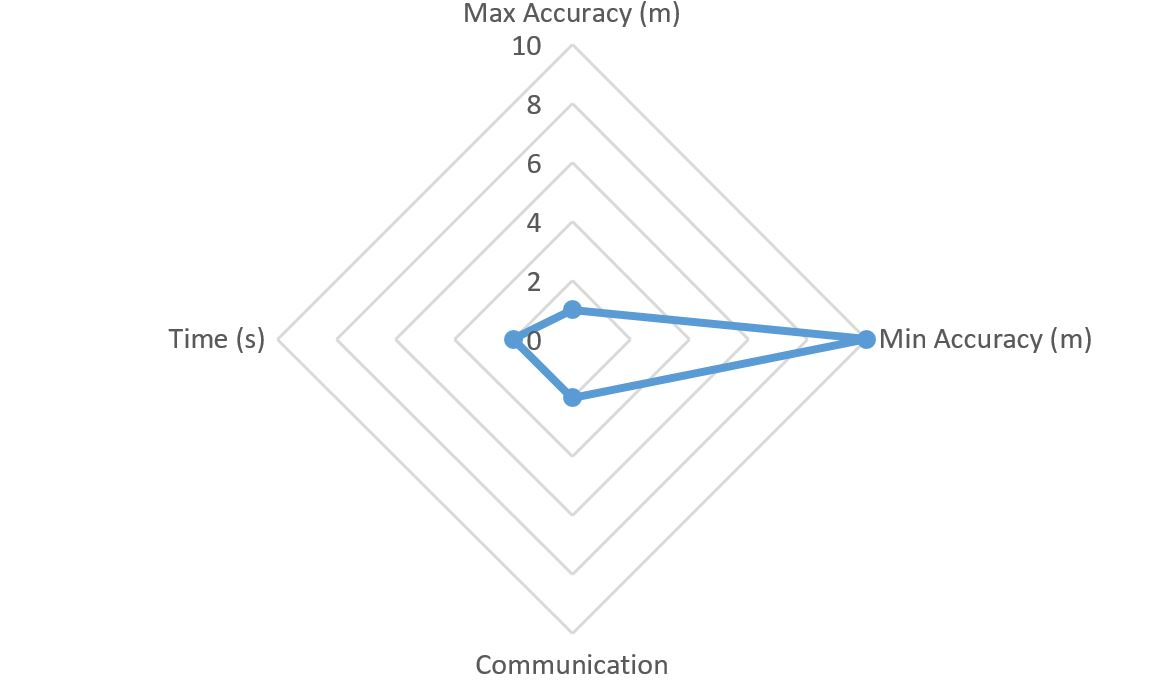
\includegraphics[width=0.6\linewidth]{Chapters/Figures/bleradar.jpg}}%

 % \caption{BLE Results}
  %\label{fig:BLE_radar}
%\end{figure}


\begin{table}[htbp]
\centering
\begin{tabular}{@{}ccccc@{}}
\toprule
 & Max accuracy & Min Accuracy & Communication &   \hspace{0.7cm}Time\hspace{0.7cm}    \\ \midrule
\begin{tabular}[c]{@{}c@{}}BLE \\ Indoor\end{tabular} & 1 m & 10 m & No & 4 s\\ \bottomrule
\end{tabular}
\caption{BLE Results}
\label{tab:BLE_Res}
\end{table}



%%%%%%%%%%%%%%%%%%%%%% Sub sec GNSS  %%%%%%%%%%%%%%%%%%%%%%%%%%%%%%%%%%%
\newpage
\subsubsection{GNSS}
\label{subsubsec:Geo_GNSS}
During the development phase in the laboratory scenario, the results obtained for the GNSS were done using one FiPy and one Pytrack shield. The Pytrack~\cite{PytrackSpecs} shield has a Quectel GNSS L76-L~\cite{quectel,quectelspecs}, this receiver module supports Multi-GNSS including GPS, GLONASS, Galileo and QZSS systems. The antenna used for the GNSS system was the one from the shield (surface mounted 6 by 2 mm) and not an external one due to the design dimension constrains.

The test consisted initially to obtain an indoor position, which as expected failed. The test was then conducted outdoor using LoRa as communication method, and at stationary speeds, the results obtained are expressed in the next figure~\ref{fig:GNSS_points}.

\begin{figure}[htbp]
  \centering

    {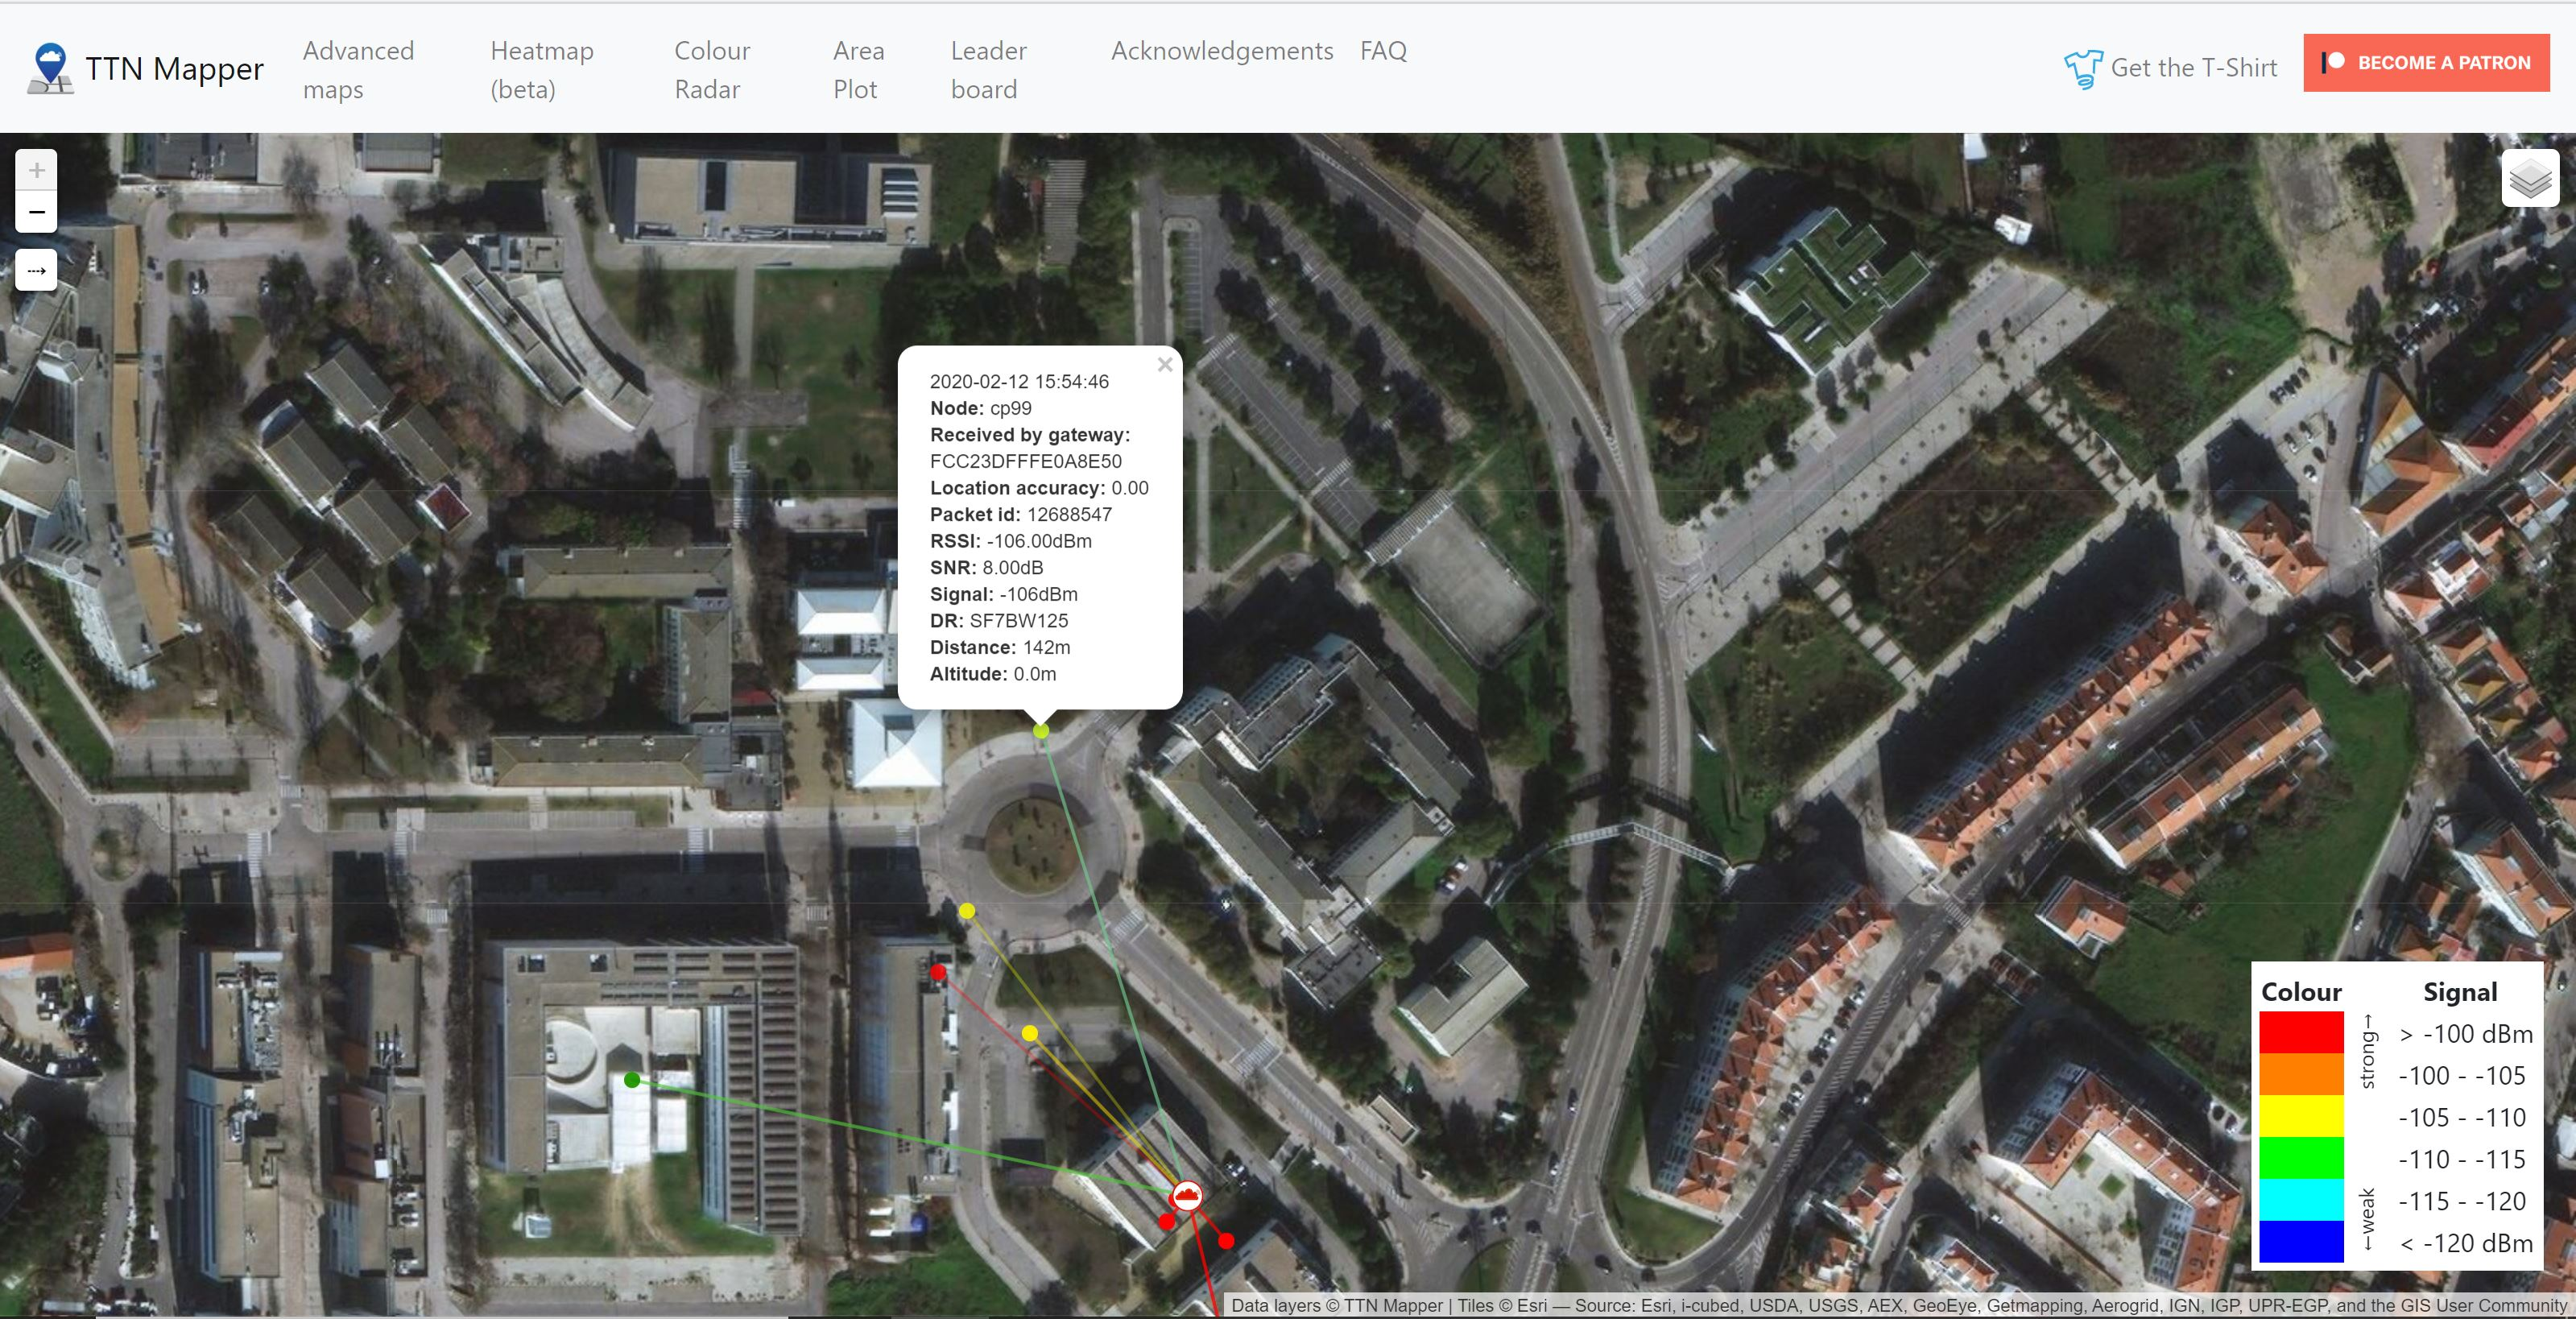
\includegraphics[width=0.7\linewidth]{Chapters/Figures/ttnmappergps.JPG}}%

  \caption{GNSS }
  \label{fig:GNSS_points}
\end{figure}

The next test consisted of getting  GNSS Location while walking, considering the walking speed of 5km/h, to simulate a tracking situation. The TTFF (Time to first fix) announced is between 1 to 35 seconds, the one from the tests is more close to 120 seconds from a cold a start. The result from using the device in a clear day and waiting for 5 minutes to fix position, and then start walking was good but often during 40 minutes walk the device misses some points, some points return the location empty. This can be due to the fact the GNSS has 33 channels for tracking and 99 for the acquisition of the location. The problem verified with the requisitions of the location could be solved by using an external antenna.

%%%IMPORTANTE !
%%%%(se calhar por a aqui pontos estacionarios e não tracking , ficar para baixo)


%\begin{figure}[htbp]
%  \centering

%    {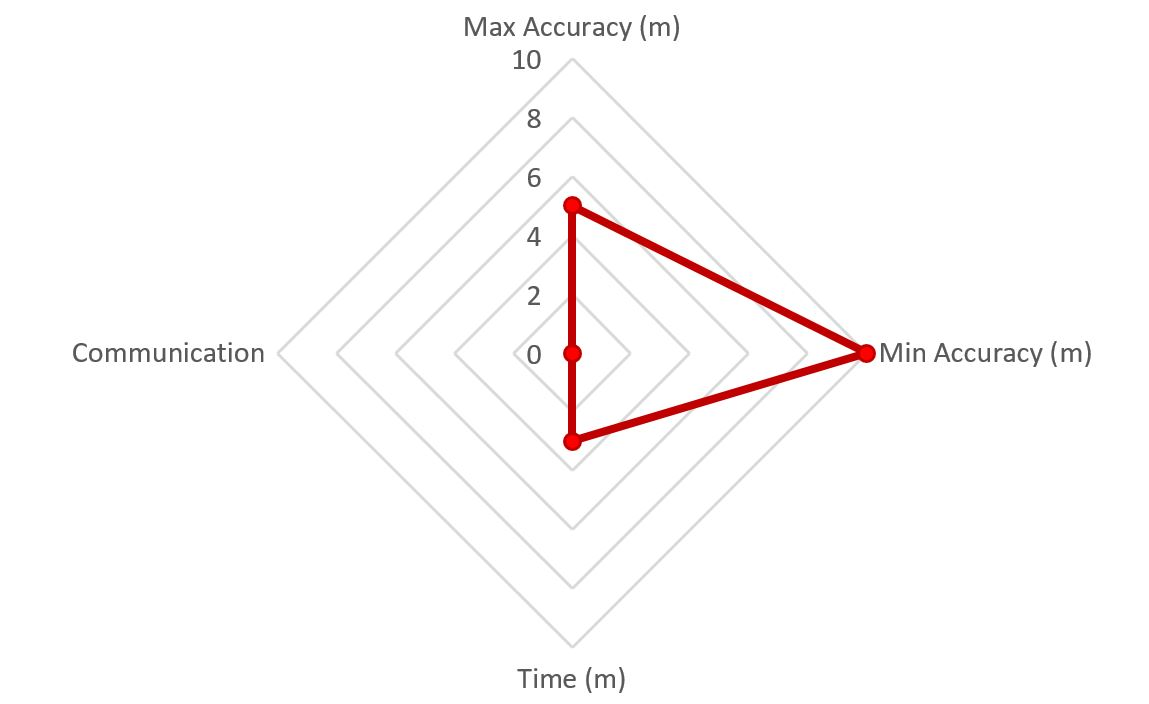
\includegraphics[width=0.5\linewidth]{Chapters/Figures/gnssradar.JPG}}%

%  \caption{GNSS}
%  \label{fig:GNSS_radar}
%\end{figure}


The location accuracy is from ($<2,5 to 11$) 5 m to 10 m. The time used to retrieve the first location after a cold start was approximately $120$ seconds, and the GNSS cannot be used to transmit the full Status message. The next table~\ref{tab:GNSS_Res} represents the resume of this geolocation technique.\newline

\begin{table}[htbp]
\centering
\begin{tabular}{@{}ccccc@{}}
\toprule
 & Max accuracy & Min Accuracy & Communication &    \hspace{0.7cm}Time\hspace{0.7cm}   \\ \midrule
\begin{tabular}[c]{@{}c@{}}GNSS \\ Outdoor\end{tabular} & 5 m & 10 m & No & 120* s\\ \bottomrule
\end{tabular}
\caption{GNSS Results}
\label{tab:GNSS_Res}
\end{table}



%##########################################   WIFI GEO sub sec
\subsubsection{WiFi}
\label{subsubsec:Geo_WiFi}

The following Geolocation method tested was the WiFi assisted location. For this experiment was used the same FiPy as above, in the belt box enclosure. The WiFi antenna used was the internal one. For the software was used the Geolocation API from Google.

The test consisted of one FiPy mobile that was simulating the patient. The test took place indoor. Since it was first tested using WiFi as a communication method, therefore the maximum coverage of the WiFi AP only permitted indoor usage and just a bit outdoor.

\begin{figure}[htbp]
  \centering

    {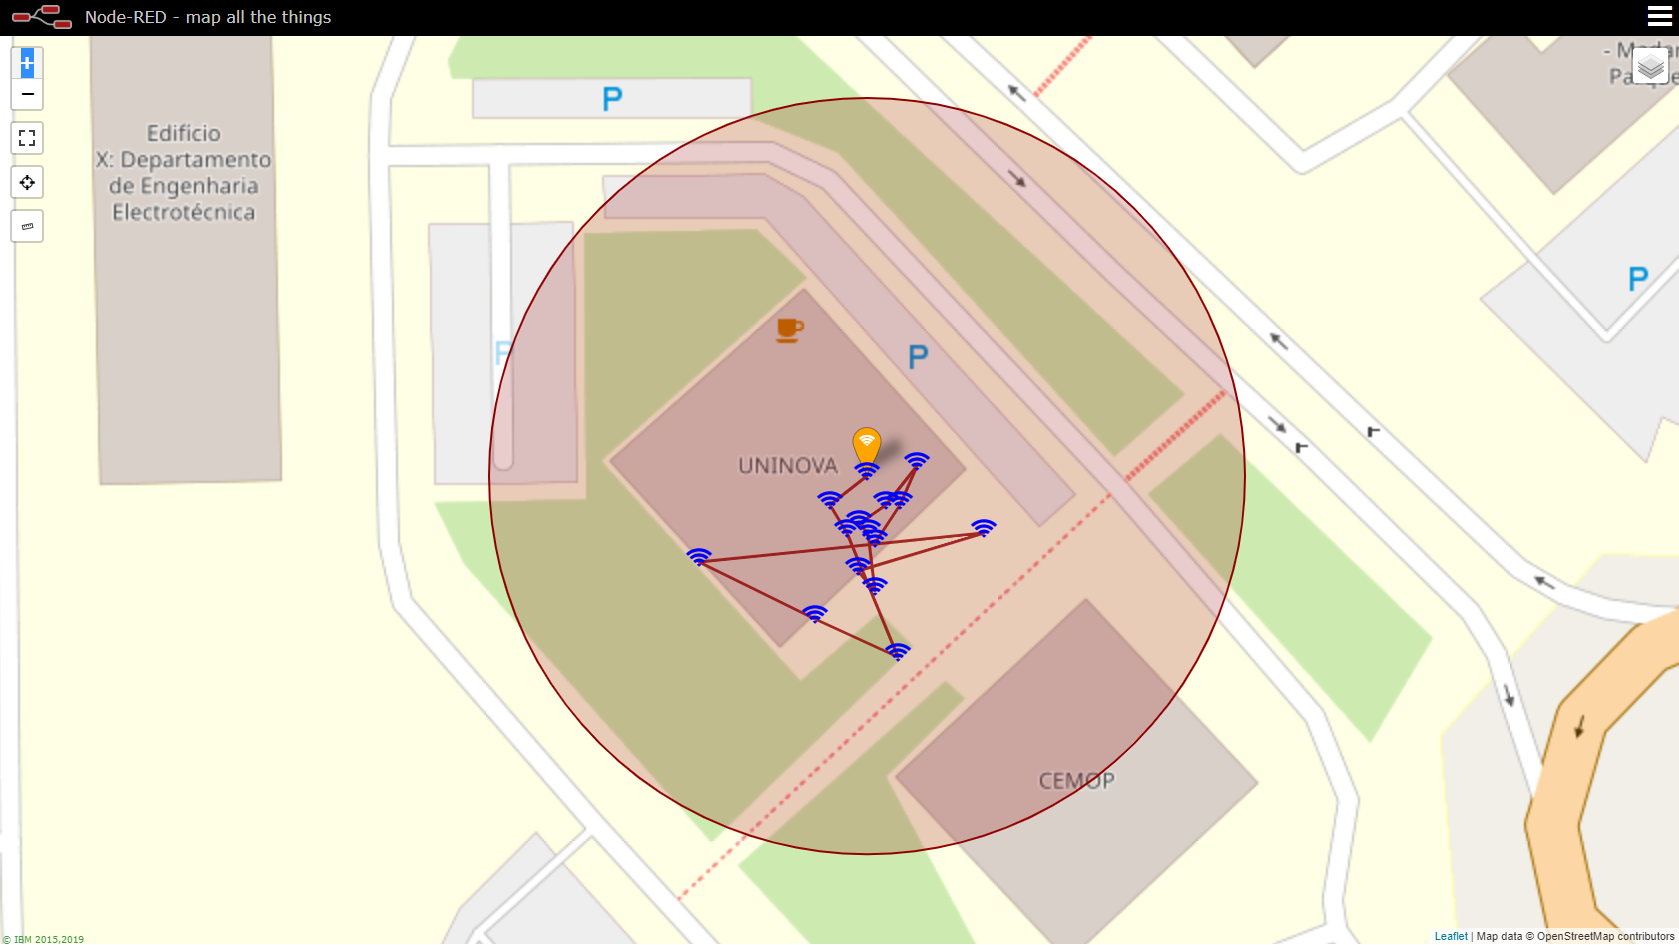
\includegraphics[width=0.6\linewidth]{Chapters/Figures/wifilab.png}}%

  \caption{WiFi lab}
  \label{fig:WiFi_geo}
\end{figure}
In the device side, there was a scan for WiFi APs. The device started by reading the values from the APs (access points or routers). These values consisted of SSID (service set identifier) which is the WiFi name of the network,
BSSID (basic service set identifier) that is the  MAC address of the AP, RSSI (received signal strength indication) that is the power present in a received radio signal. There were other fields advertised such as the network channel or security, but they were all discarded since they were not useful in this situation.
After getting this information a JSON object was generated in the device, to construct a request for the google API.
The Google API then returns the approximate location as its possible to observe in the figure.~\ref{fig:WiFi_geo}.

%\begin{figure}[htbp]
%  \centering

%    {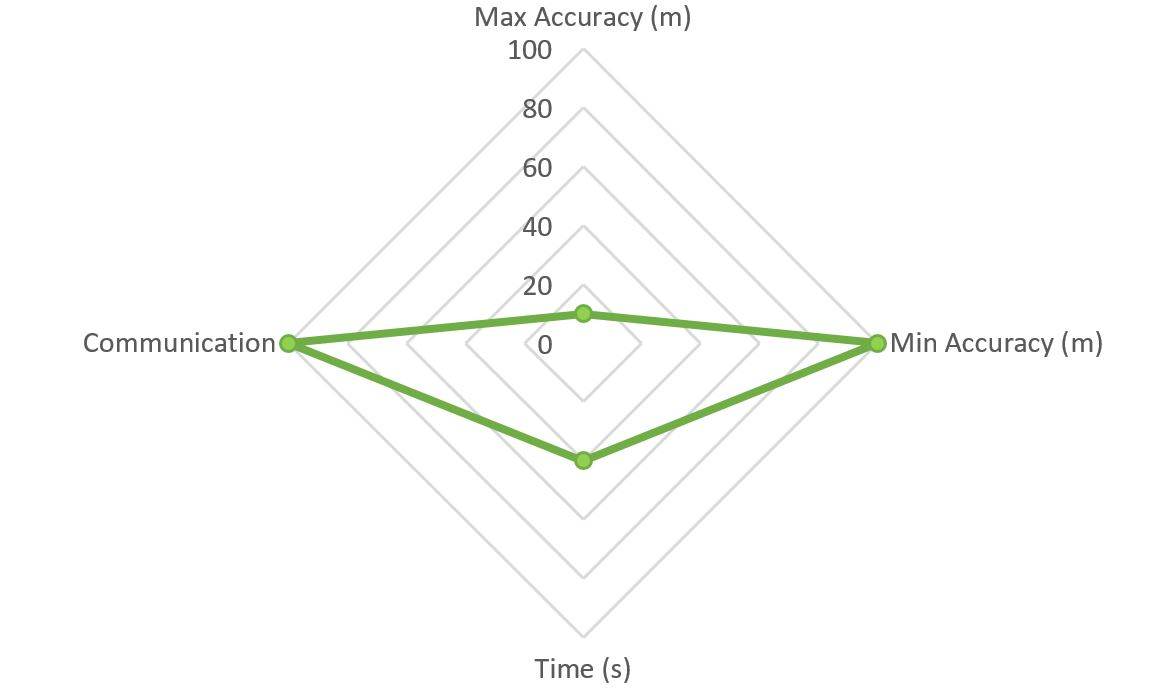
\includegraphics[width=0.5\linewidth]{Chapters/Figures/wifiradar.JPG}}%

%  \caption{WiFi}
%  \label{fig:WiFi_radar}
%\end{figure}


For this test the JSON field $considerIp$ was set to false, otherwise, Google takes the IP of the connection to identify the position, which later will not be useful when WiFi is not used as the communication technology. By doing this, was necessary to handle the errors that exist when there were no WiFi APs, or Google databases had no position information about the  previous sent WiFi APs.

The returned location accuracy was from  15 m to 100 m. The time used to retrieve the location was approximately $3$ sec, and the WiFi can be used to transmit the full Status message. The next table~\ref{tab:WIF_Res} represents the resume of this assisted geolocation technique.
\begin{table}[htbp]
\centering
\begin{tabular}{@{}ccccc@{}}
\toprule
 & Max accuracy & Min Accuracy & Communication &   \hspace{0.7cm}Time\hspace{0.7cm} \\ \midrule
\begin{tabular}[c]{@{}c@{}}WiFi \\ Indoor\end{tabular} & 15 m & 100 m & Yes & 3 s\\ \bottomrule
\end{tabular}
\caption{WiFi Results}
\label{tab:WIF_Res}
\end{table}

%##########################################
\subsubsection{LoRa}
\label{subsubsec:Geo_LoRa}
The last Geolocation method tested was LoRa as GNSS-free geolocation. For this experiment was used the same FiPy. And for the first experiment were used three other FiPy acting as gateways. The LoRa antenna used was an external one (SMA Tilt Swivel 1/2 Wave Whip Dipole). For the software was used the LoRa Cloud (formerly Collos) API from Semtech, and the TTN network server.

The first test consisted of using one FiPy mobile simulating the patient. And three others acting as gateways, for the gateways, was used the LoRaWAN Nano-Gateway example from pycom, the only issue encountered was with the internet from the campus, that was blocking the UDP packets, so the gateways were not able to sync with NTP servers and were not capable to forward the messages. This problem was solved by using a smartphone as a WiFi hot-spot. The test was conducted indoor, with the gateways separated from each other in a triangle shape. This test failed to obtain the location, mainly due to the fact the gateway were  closer than the maximum accuracy for this method. 
\begin{figure}[htbp]
  \centering
  
    {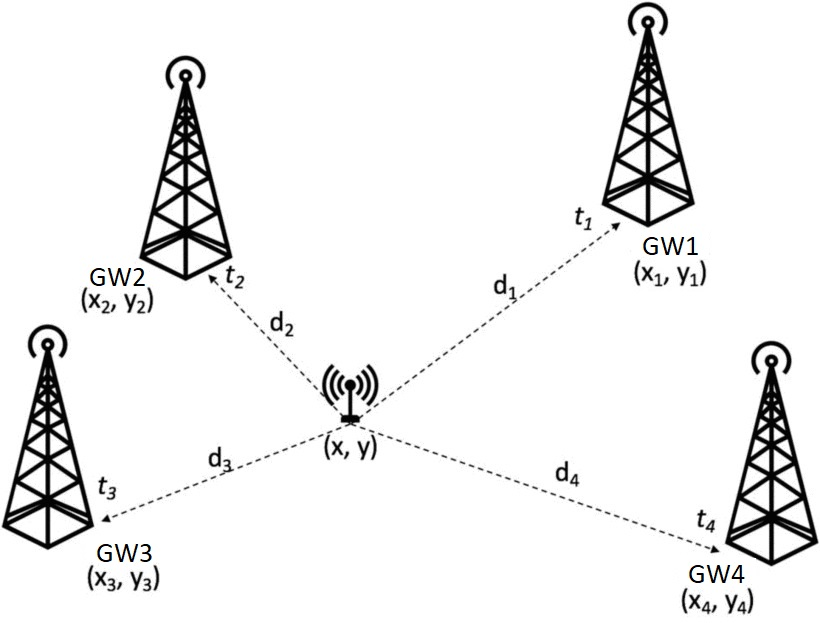
\includegraphics[width=0.5\linewidth]{Chapters/Figures/1234.jpg}}%
 
  \caption{Lora 4 Gateways Location}
  \label{fig:Lora_4GWs}
\end{figure}

The second test consisted of the same device, but now the test was conducted outdoor. For the Gateway were used three although a fourth one was also in range by using the external antenna. The figure~\ref{fig:Lora_4GWs}, describes the test scenario and the three used Gateways can be seen in the next figure~\ref{fig:LoRa_GWs}, the right one is a raspberry pi 3 with a dragino hat, on the roof of building 230 meters from the middle one. That was LoRix One at the time of the test was inside of the Uninova CTS building, and the last one 80m  was also indoor in the Electrical Engineering department and was an ESP based Gateway. The other Gateway was located in Lisbon 8km way, and it was also a LoRix one.

\begin{figure}[htbp]
  \centering

    {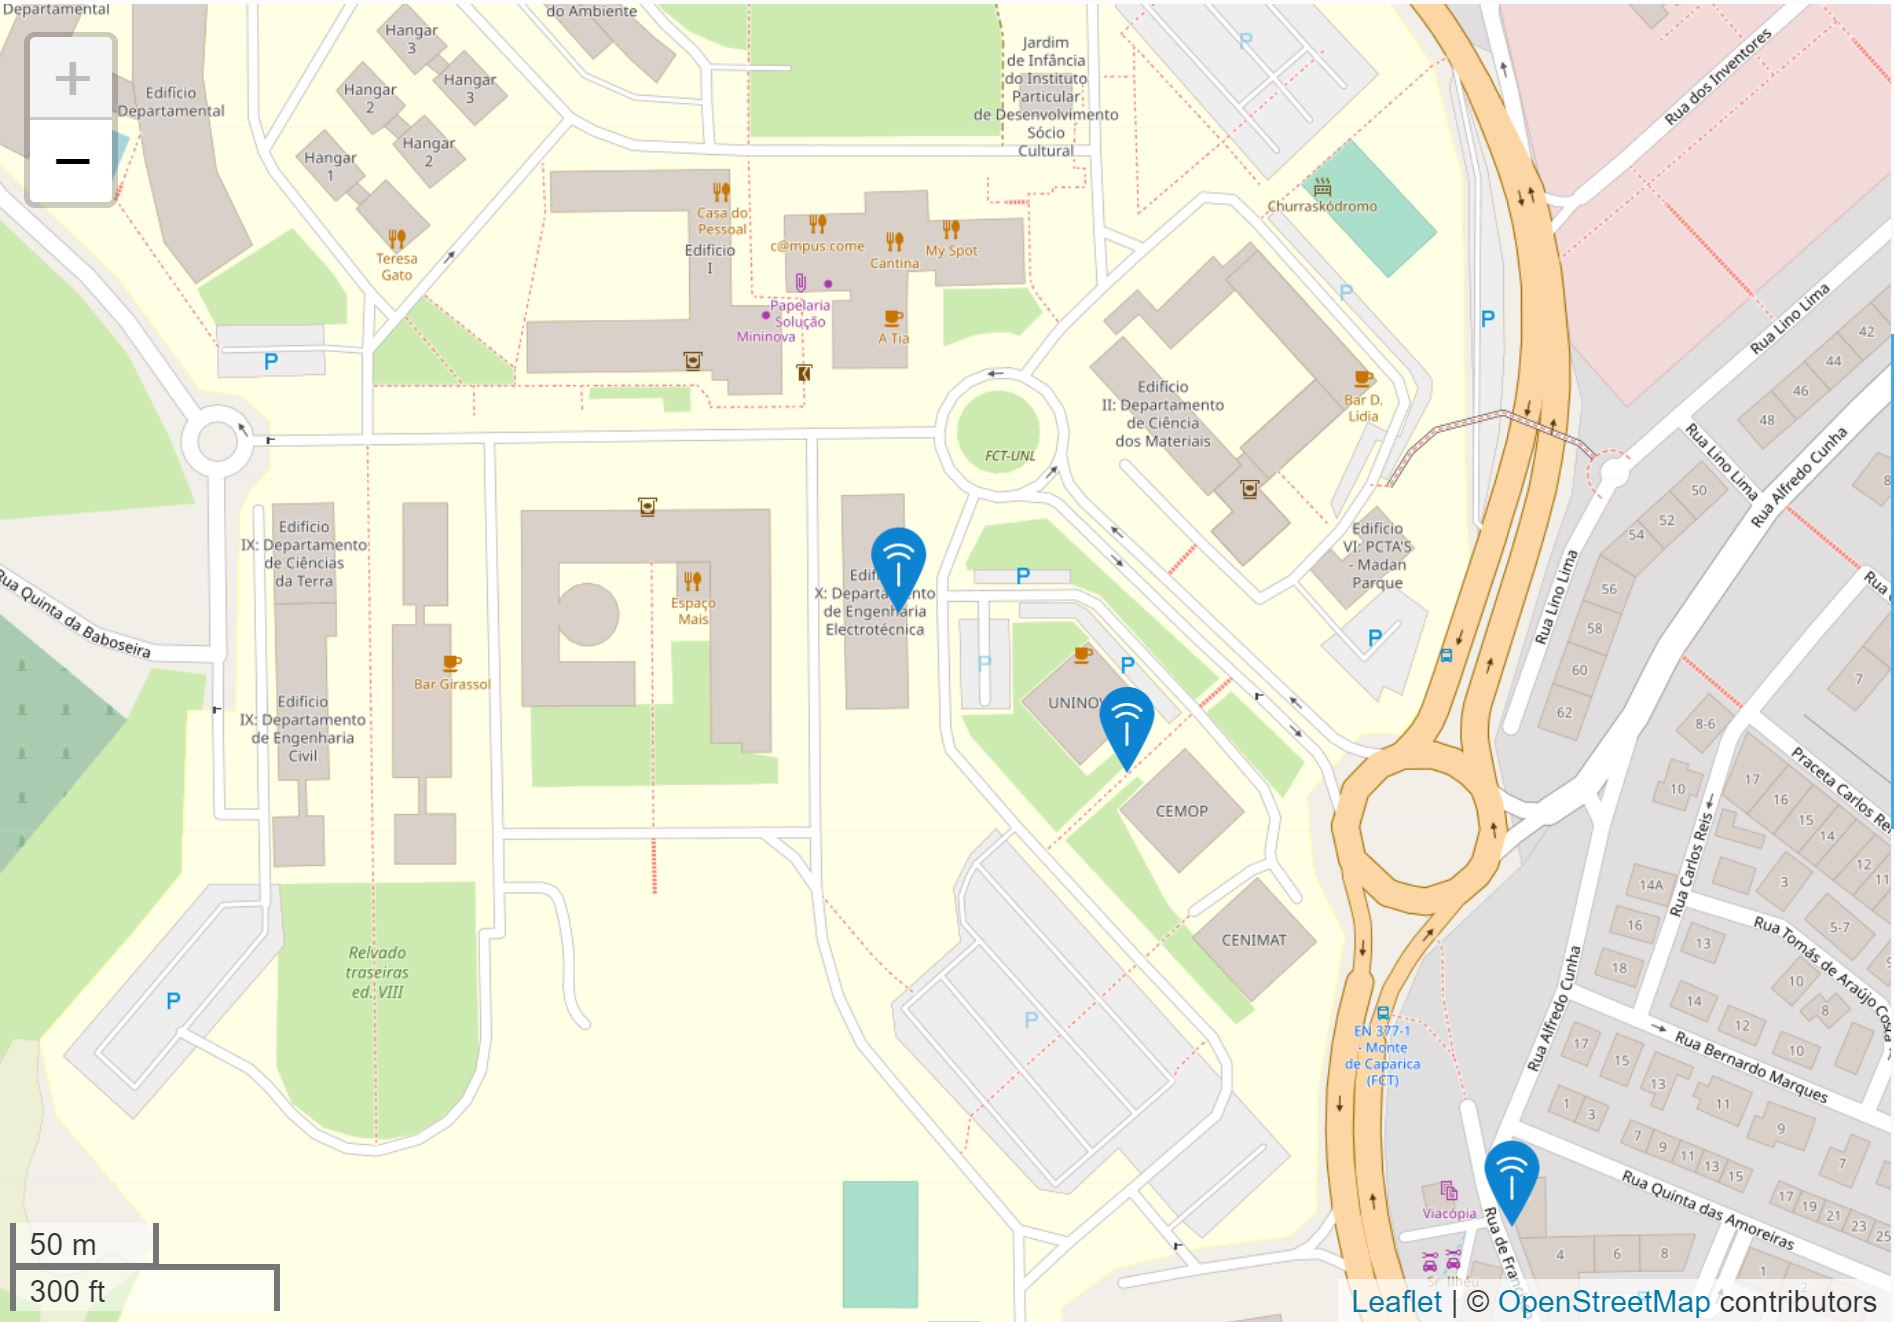
\includegraphics[width=0.59\linewidth]{Chapters/Figures/ttn3gws.JPG}}%
   %{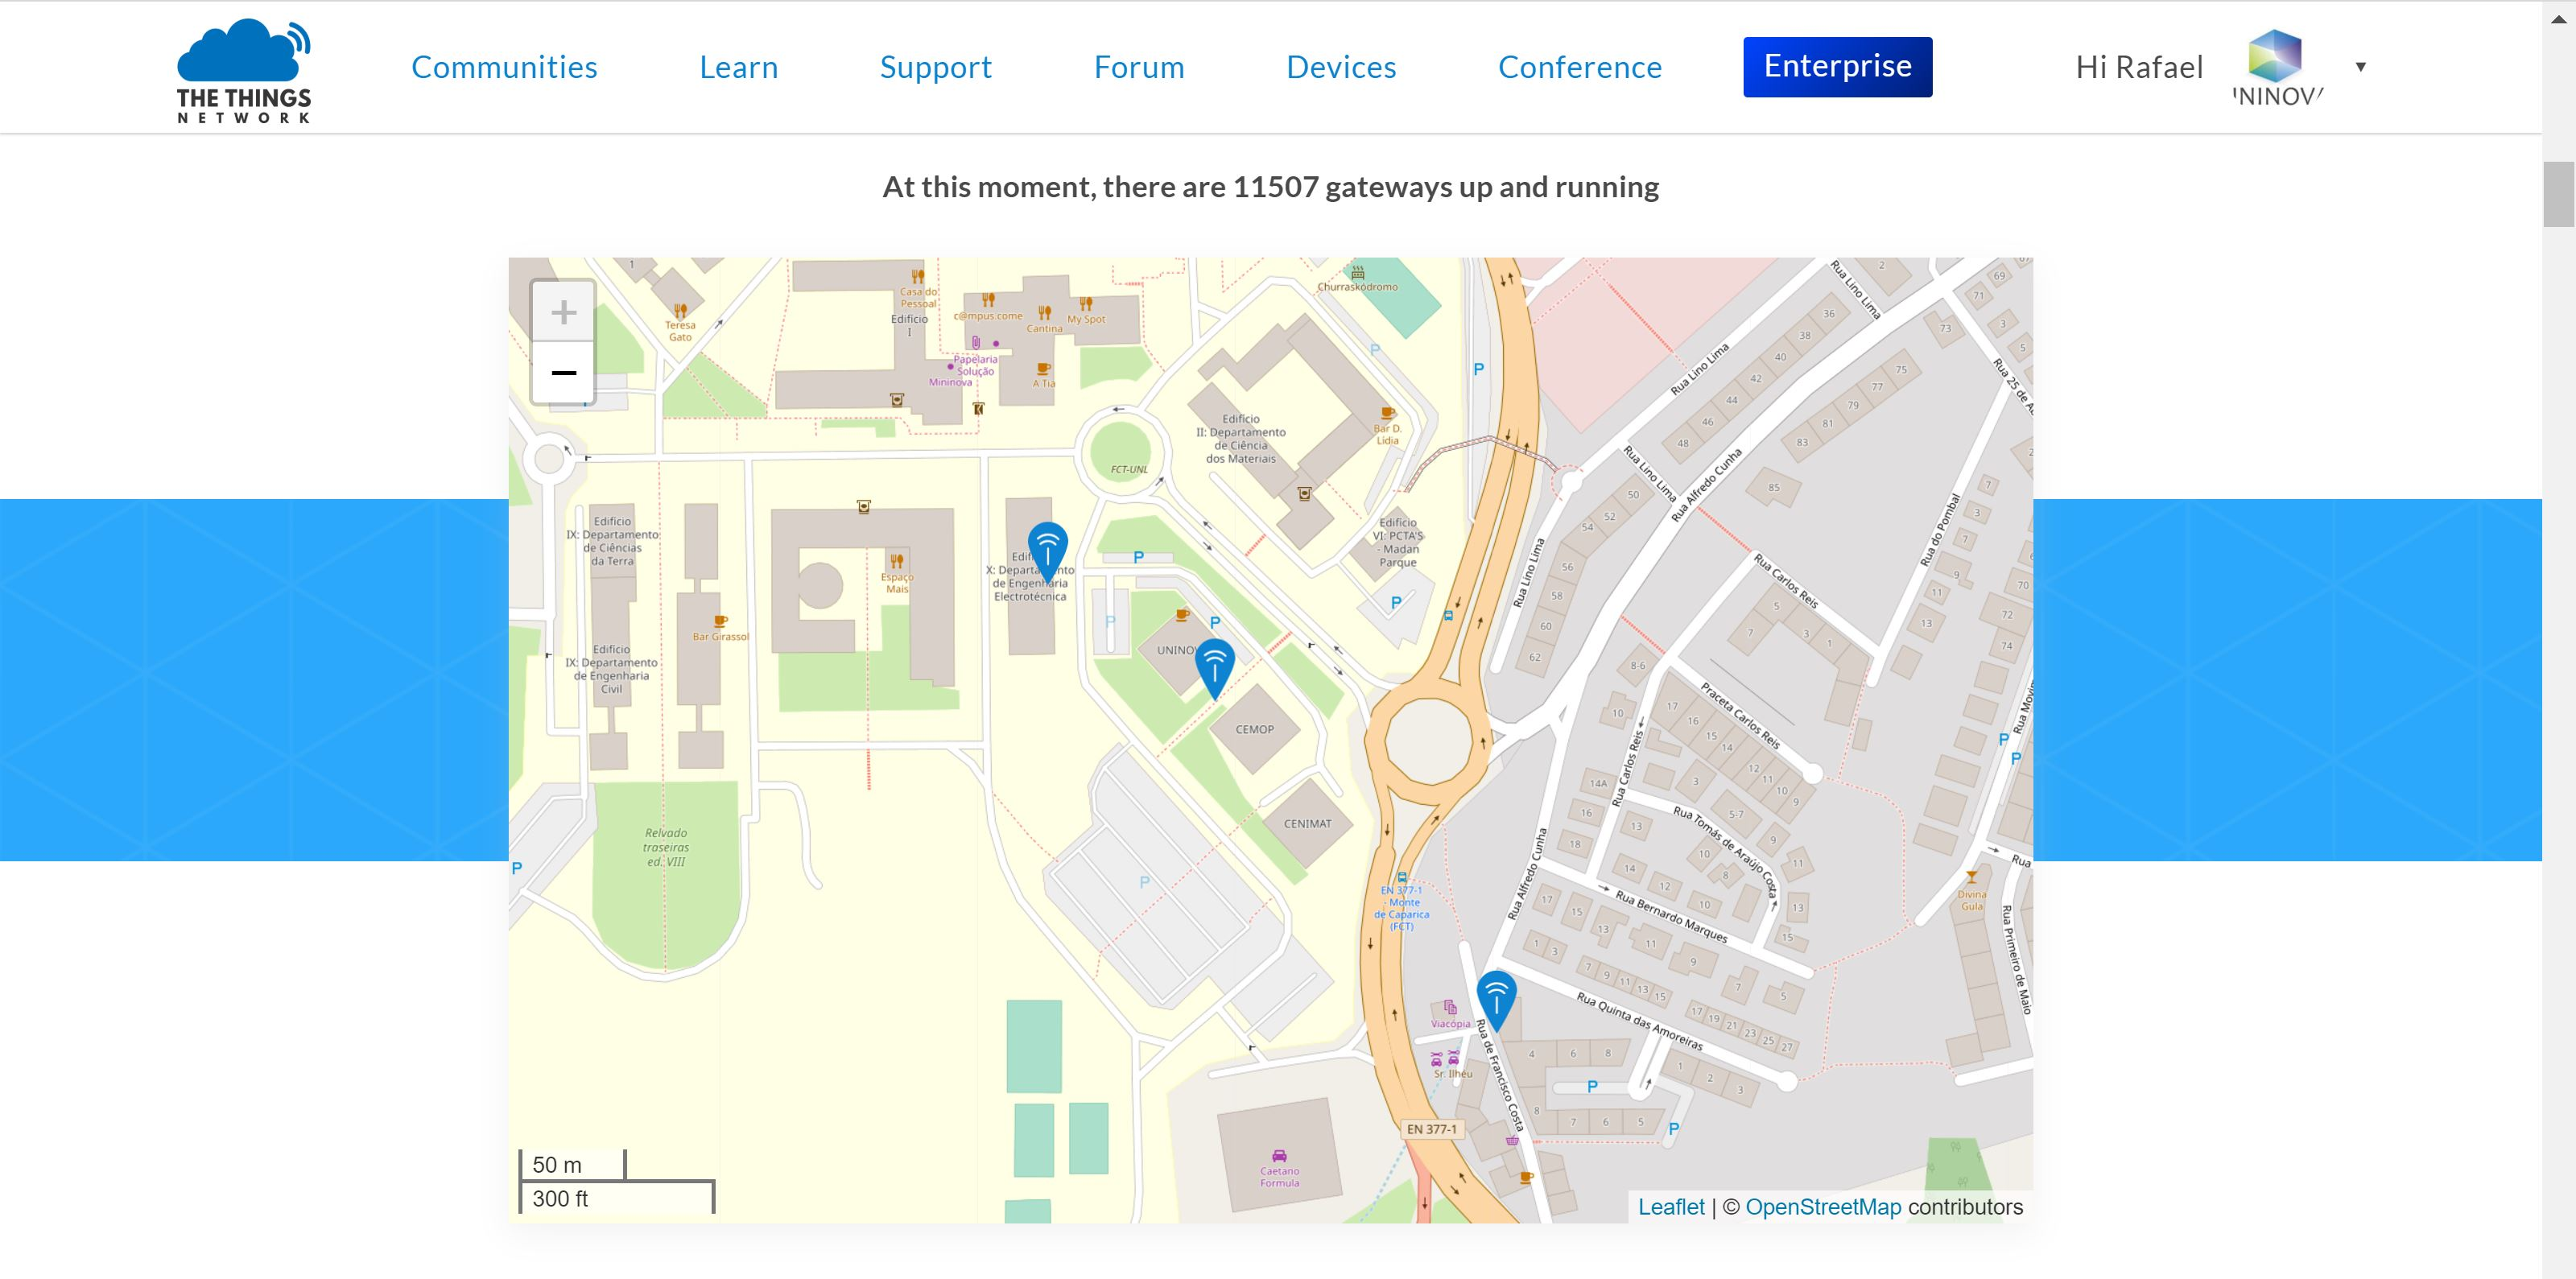
\includegraphics[width=\linewidth]{Chapters/Figures/ttngws.JPG}}%TTN Full
  \caption{LoRa GWs }
  \label{fig:LoRa_GWs}
\end{figure}

In device side was sent a small 1 byte payload with the following specifications: spreading factor 7, bandwidth 125 kHz, the first channels in 868.1 MHz and 868.3MHZ, the coding rate at 4/5 and the LoRa class as C. If it were used other specifications the results could be others, but due to the fact there were 2 single-channel gateways, the author considered that, these were the best ones to ensure all of the gateways could listen to the message.
In the gateway side was simple a packet forwarded to the TTN server. In the TTN server was an Integrations with the LoRacloud API. Using the LoRa Metadata from the messages a location was then returned, as it is possible to observe in the next figure~\ref{fig:LoRa_geo_lab}.
\begin{figure}[htbp]
  \centering

    {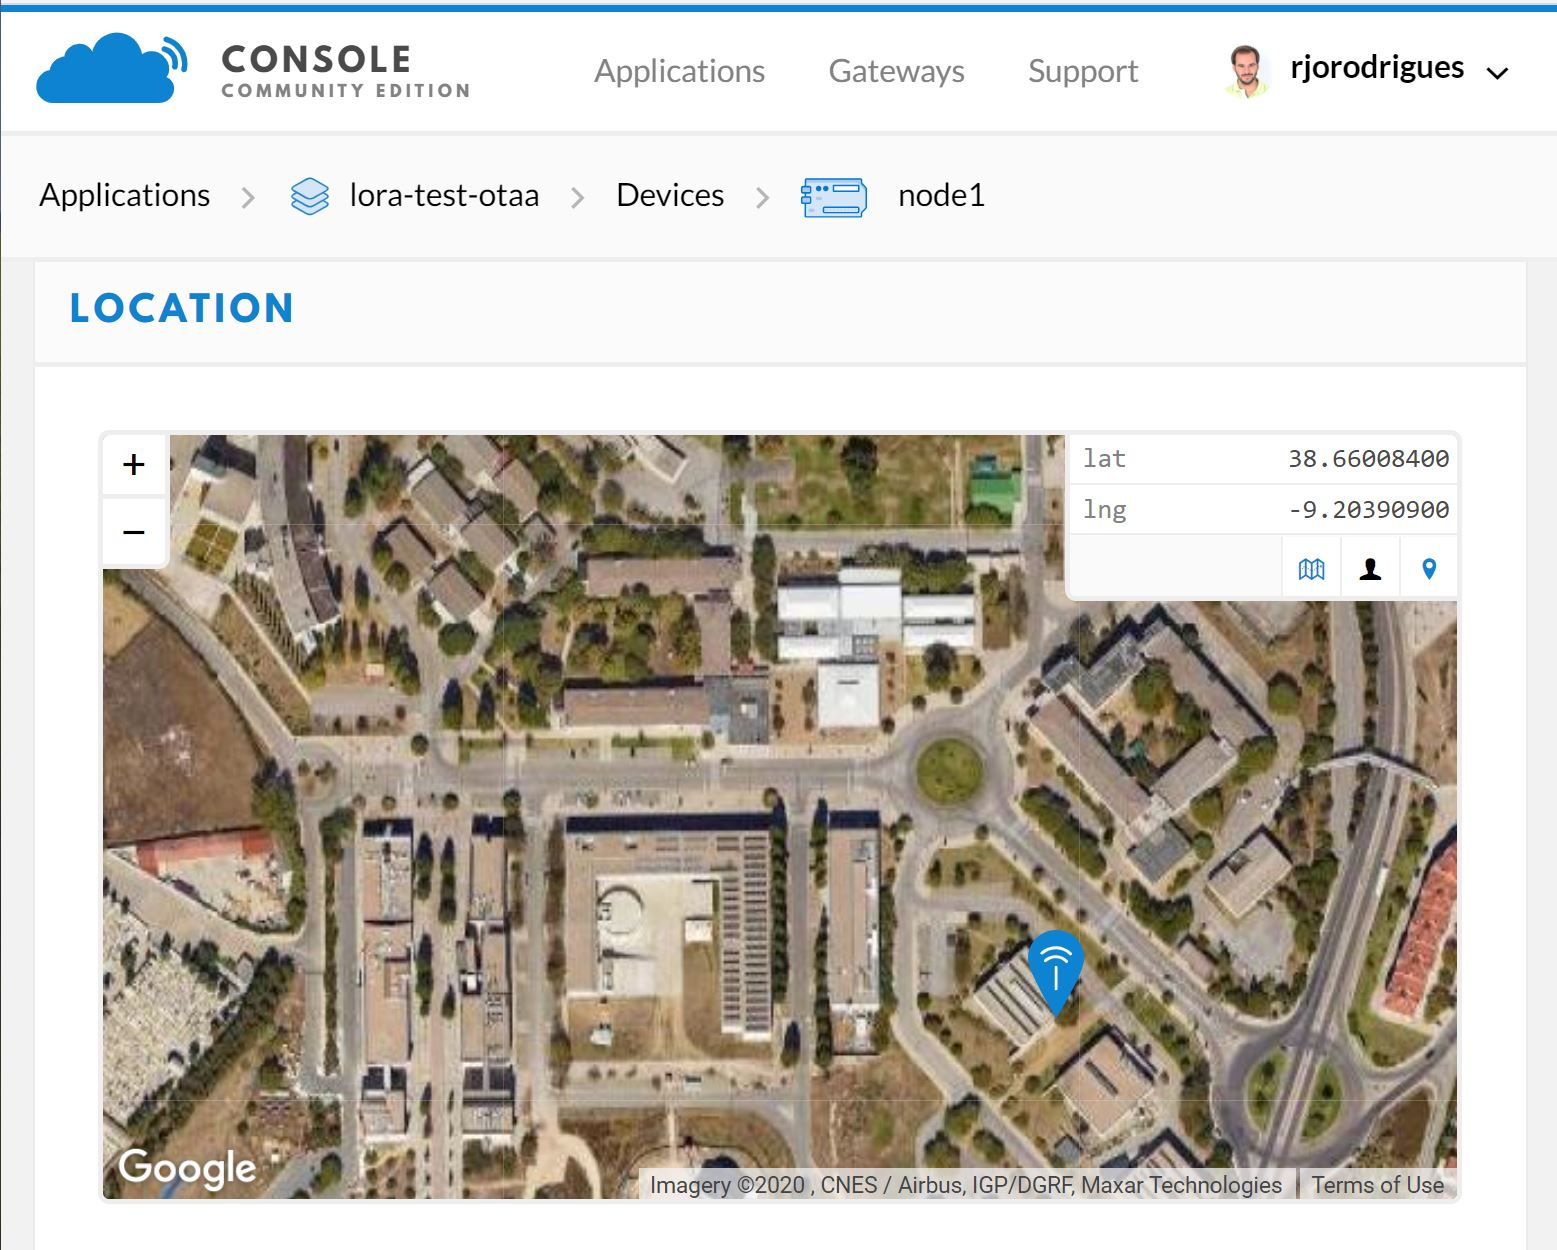
\includegraphics[width=0.59\linewidth]{Chapters/Figures/loralab.JPG}}%

  \caption{LoRa lab}
  \label{fig:LoRa_geo_lab}
  \end{figure}
  
The returned location accuracy was from  20 m to 200 m. The time used to retrieve the location was approximately $2$ sec, and LoRa was used to transmit the Status message, although was not the full status message, it was only the full values from the Status message, these values were later constructed in the TTN Network server. The next table~\ref{tab:LoRa_Res} represents the resume of this GNNS-Free geolocation technique.

%\begin{figure}[htbp]
%  \centering

%    {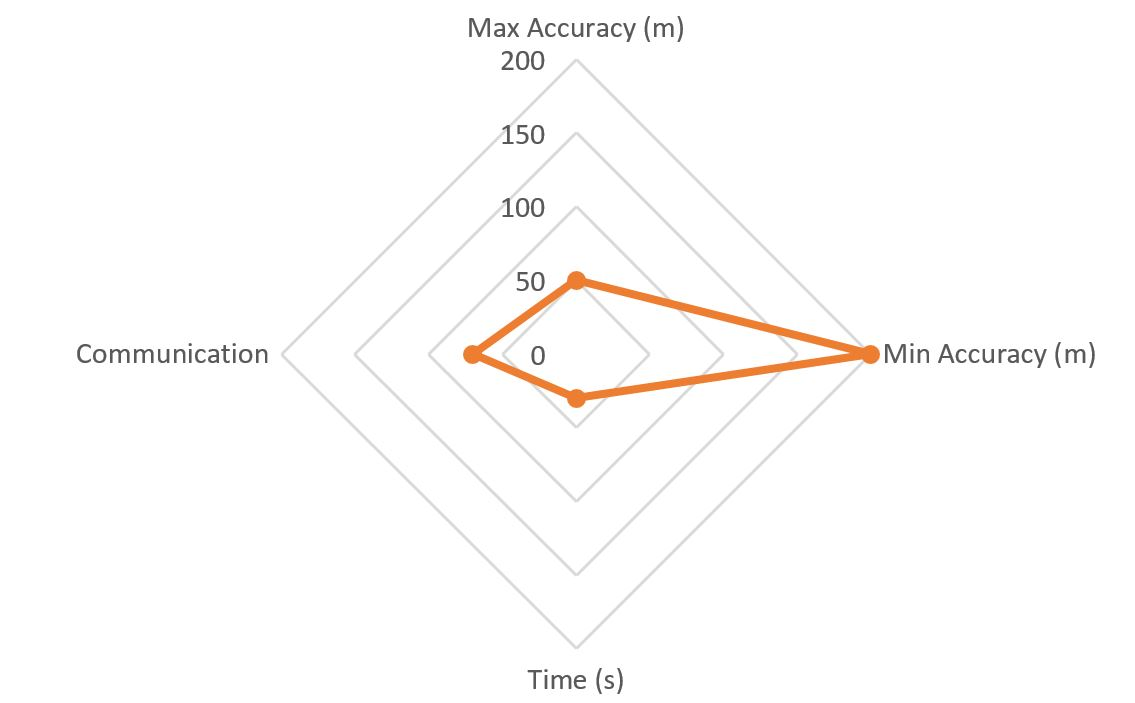
\includegraphics[width=0.5\linewidth]{Chapters/Figures/loraradar.JPG}}%

%  \caption{LoRa Results}
%%  \label{fig:LoRa_radar}
%\end{figure}

\begin{table}[htbp]
\centering
\begin{tabular}{@{}ccccc@{}}
\toprule
 & Max accuracy & Min Accuracy & Communication &   \hspace{0.7cm}Time\hspace{0.7cm} \\ \midrule
\begin{tabular}[c]{@{}c@{}}LoRa \\ Outdoor\end{tabular} & 20 m & 200 m & Yes & 2 s\\ \bottomrule
\end{tabular}
\caption{LoRa Results}
\label{tab:LoRa_Res}
\end{table}

%\subsubsection{Other GeoLocation}
%\label{subsubsec:Other_Geo}
%\paragraph{NB-IoT}
%\paragraph{SigFox}



%%%%%%%%%%%%%%%%%%%%%%%  End use case 1  %%%%%%%%%%%%%%%%%%%%%%%%%%%%%%%%%











%%%%%%%%%%%%%%%%%%%%%  Start use case 2  %%%%%%%%%%%%%%%%%%%%%%%%%%%%%%%%%%
%################### REAL WORLD ##################
\newpage

\subsection{Lisboa- Real World}
\label{subsec:real_world}
The second use case described for this section is the Real World. This use case  was separated into two test locations. The first one intended to test the results from the lab but in the urban environment, which took place in Lisbon. The second location was Alenquer (40 km away from Lisbon) to simulate the  rural environment. 


\subsubsection{GNSS}
\label{subsubsec:GNSS}

The GNSS test, in this scenario, used the same material as above in~\ref{subsubsec:Geo_GNSS}. The communication method used in this case was NB-IoT. And the test consisted of gathering GNSS Location during walking, the average speed was 5km/h, to test a real tracking situation. GNSS took about two minutes to acquire a position after a cold start.
The result of using the device in a clear day, after waiting for around 5 minutes to fix position, and then start walking are possible to observe in the next figure~\ref{fig:GNSS_Results}, on the left side~\ref{fig:GPS_Path} is the registered GNSS path, and on the right is the real path~\ref{fig:GPS_Real}.  The walk last for 50 minutes with a 4.3 km distance (about 100 location points), in a rural environment non-stop, so none of the locations points is from stationary locations. Comparing both figures is possible to observe that some points are missing, this occurred during the reacquisition of the location since the sample time was 30 seconds. The problem verified with the requisitions of the location can be solved by using an external and more powerful (higher gain) antenna.
\begin{figure}[htbp]
  \centering
  \subcaptionbox{GNSS path \label{fig:GPS_Path}}%
    {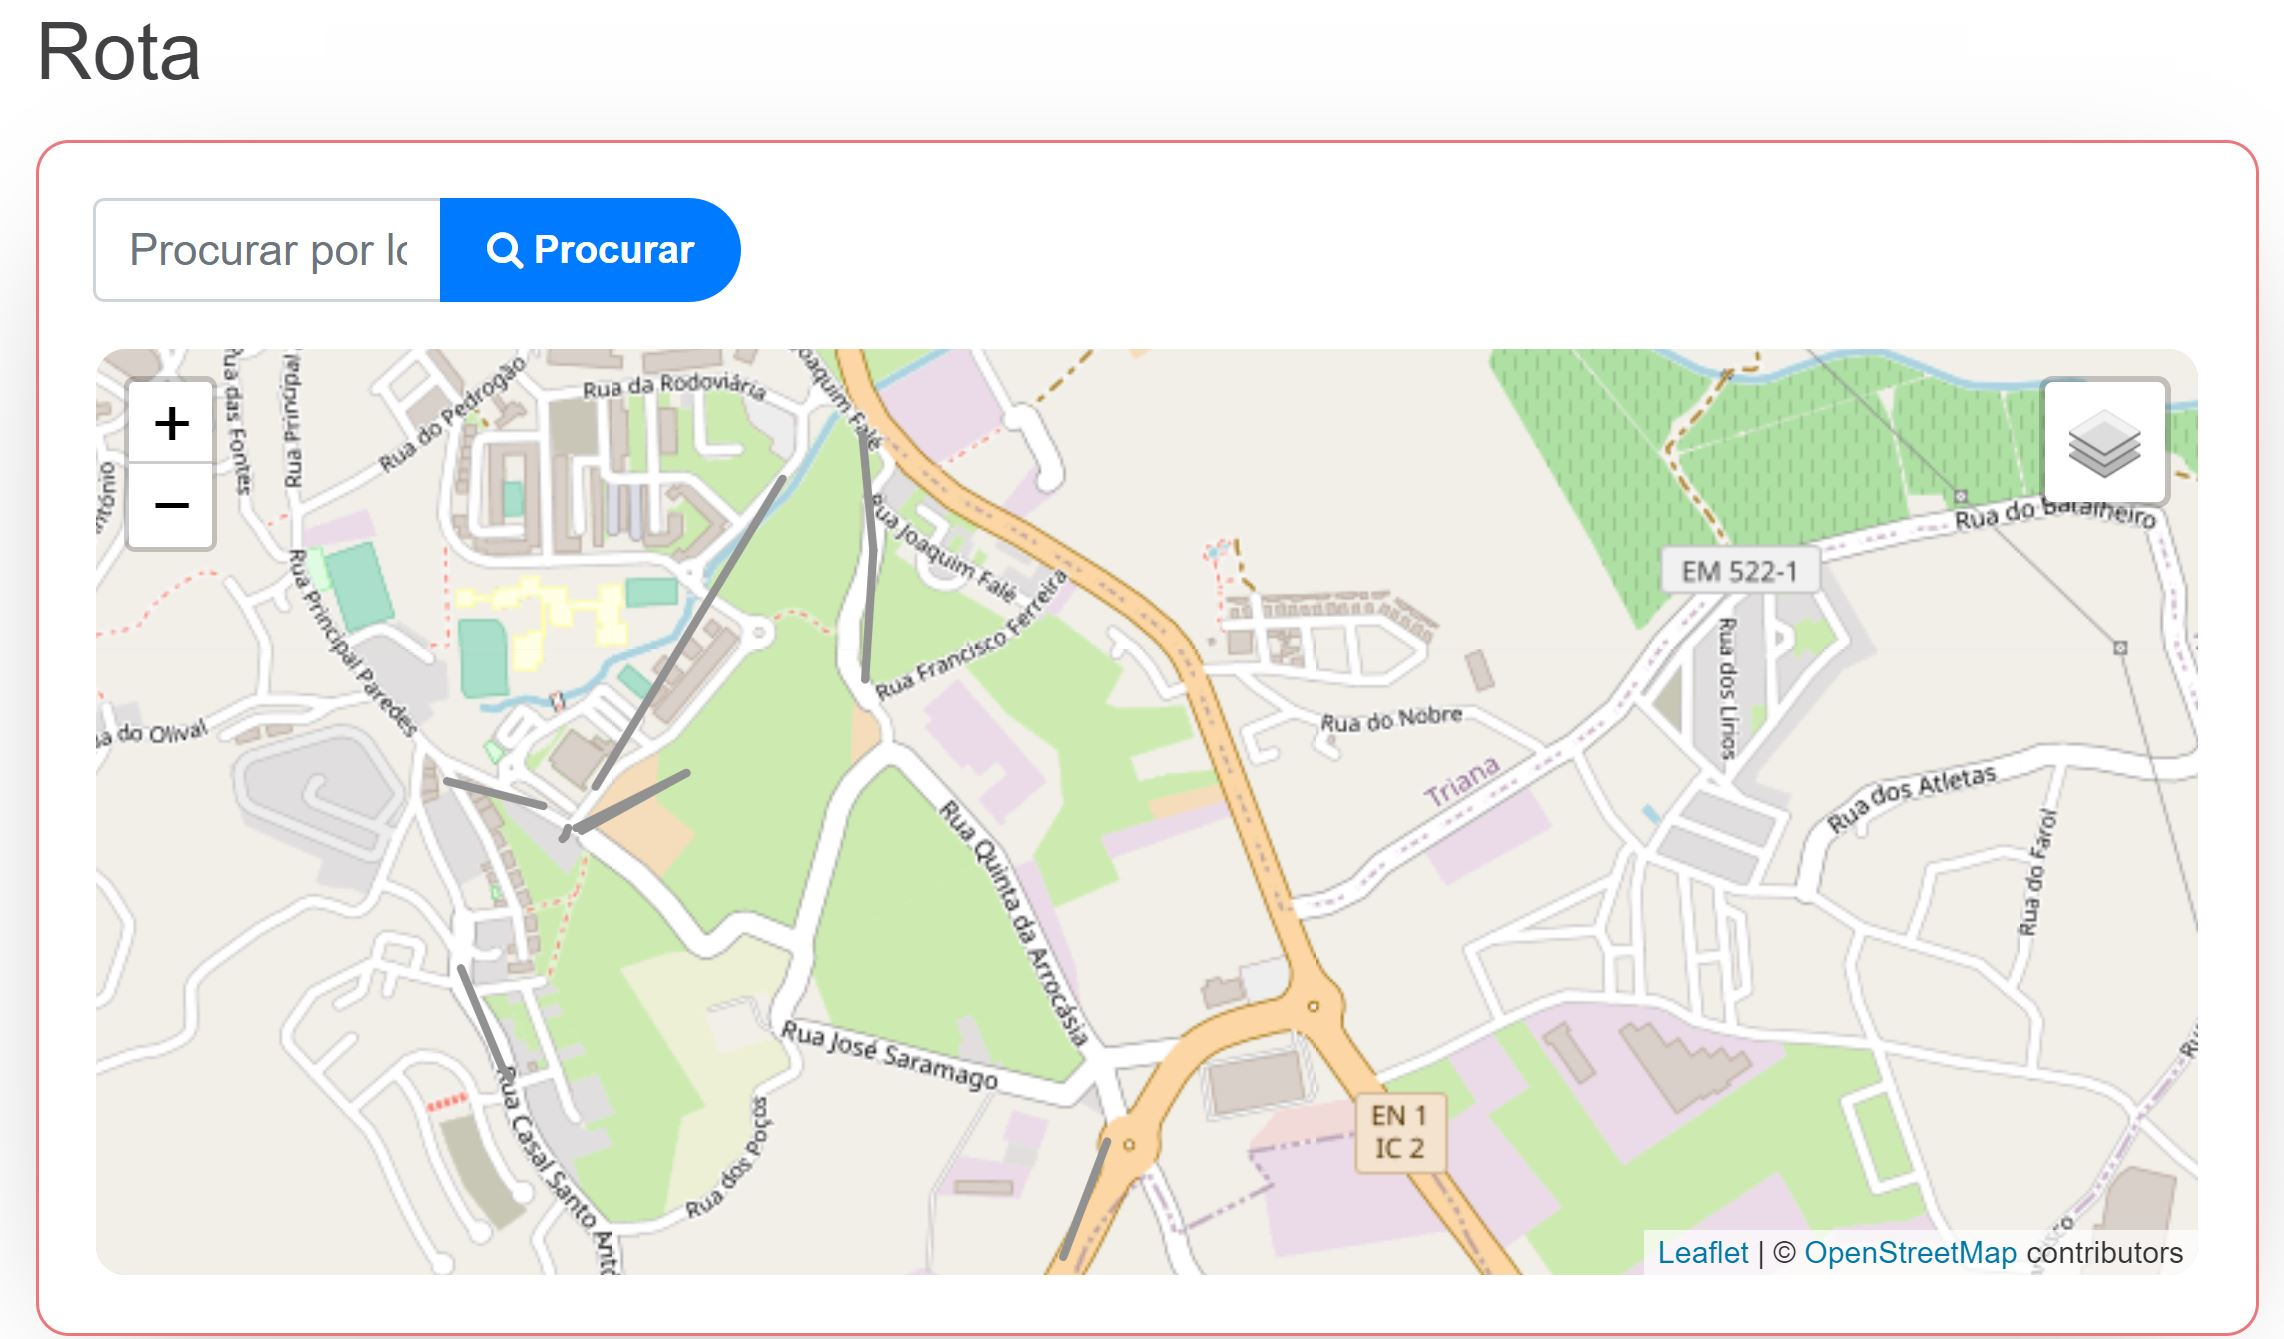
\includegraphics[width=0.5\linewidth]{Chapters/Figures/GPS.JPG}}%
  \subcaptionbox{Real path\label{fig:GPS_Real}}%
    {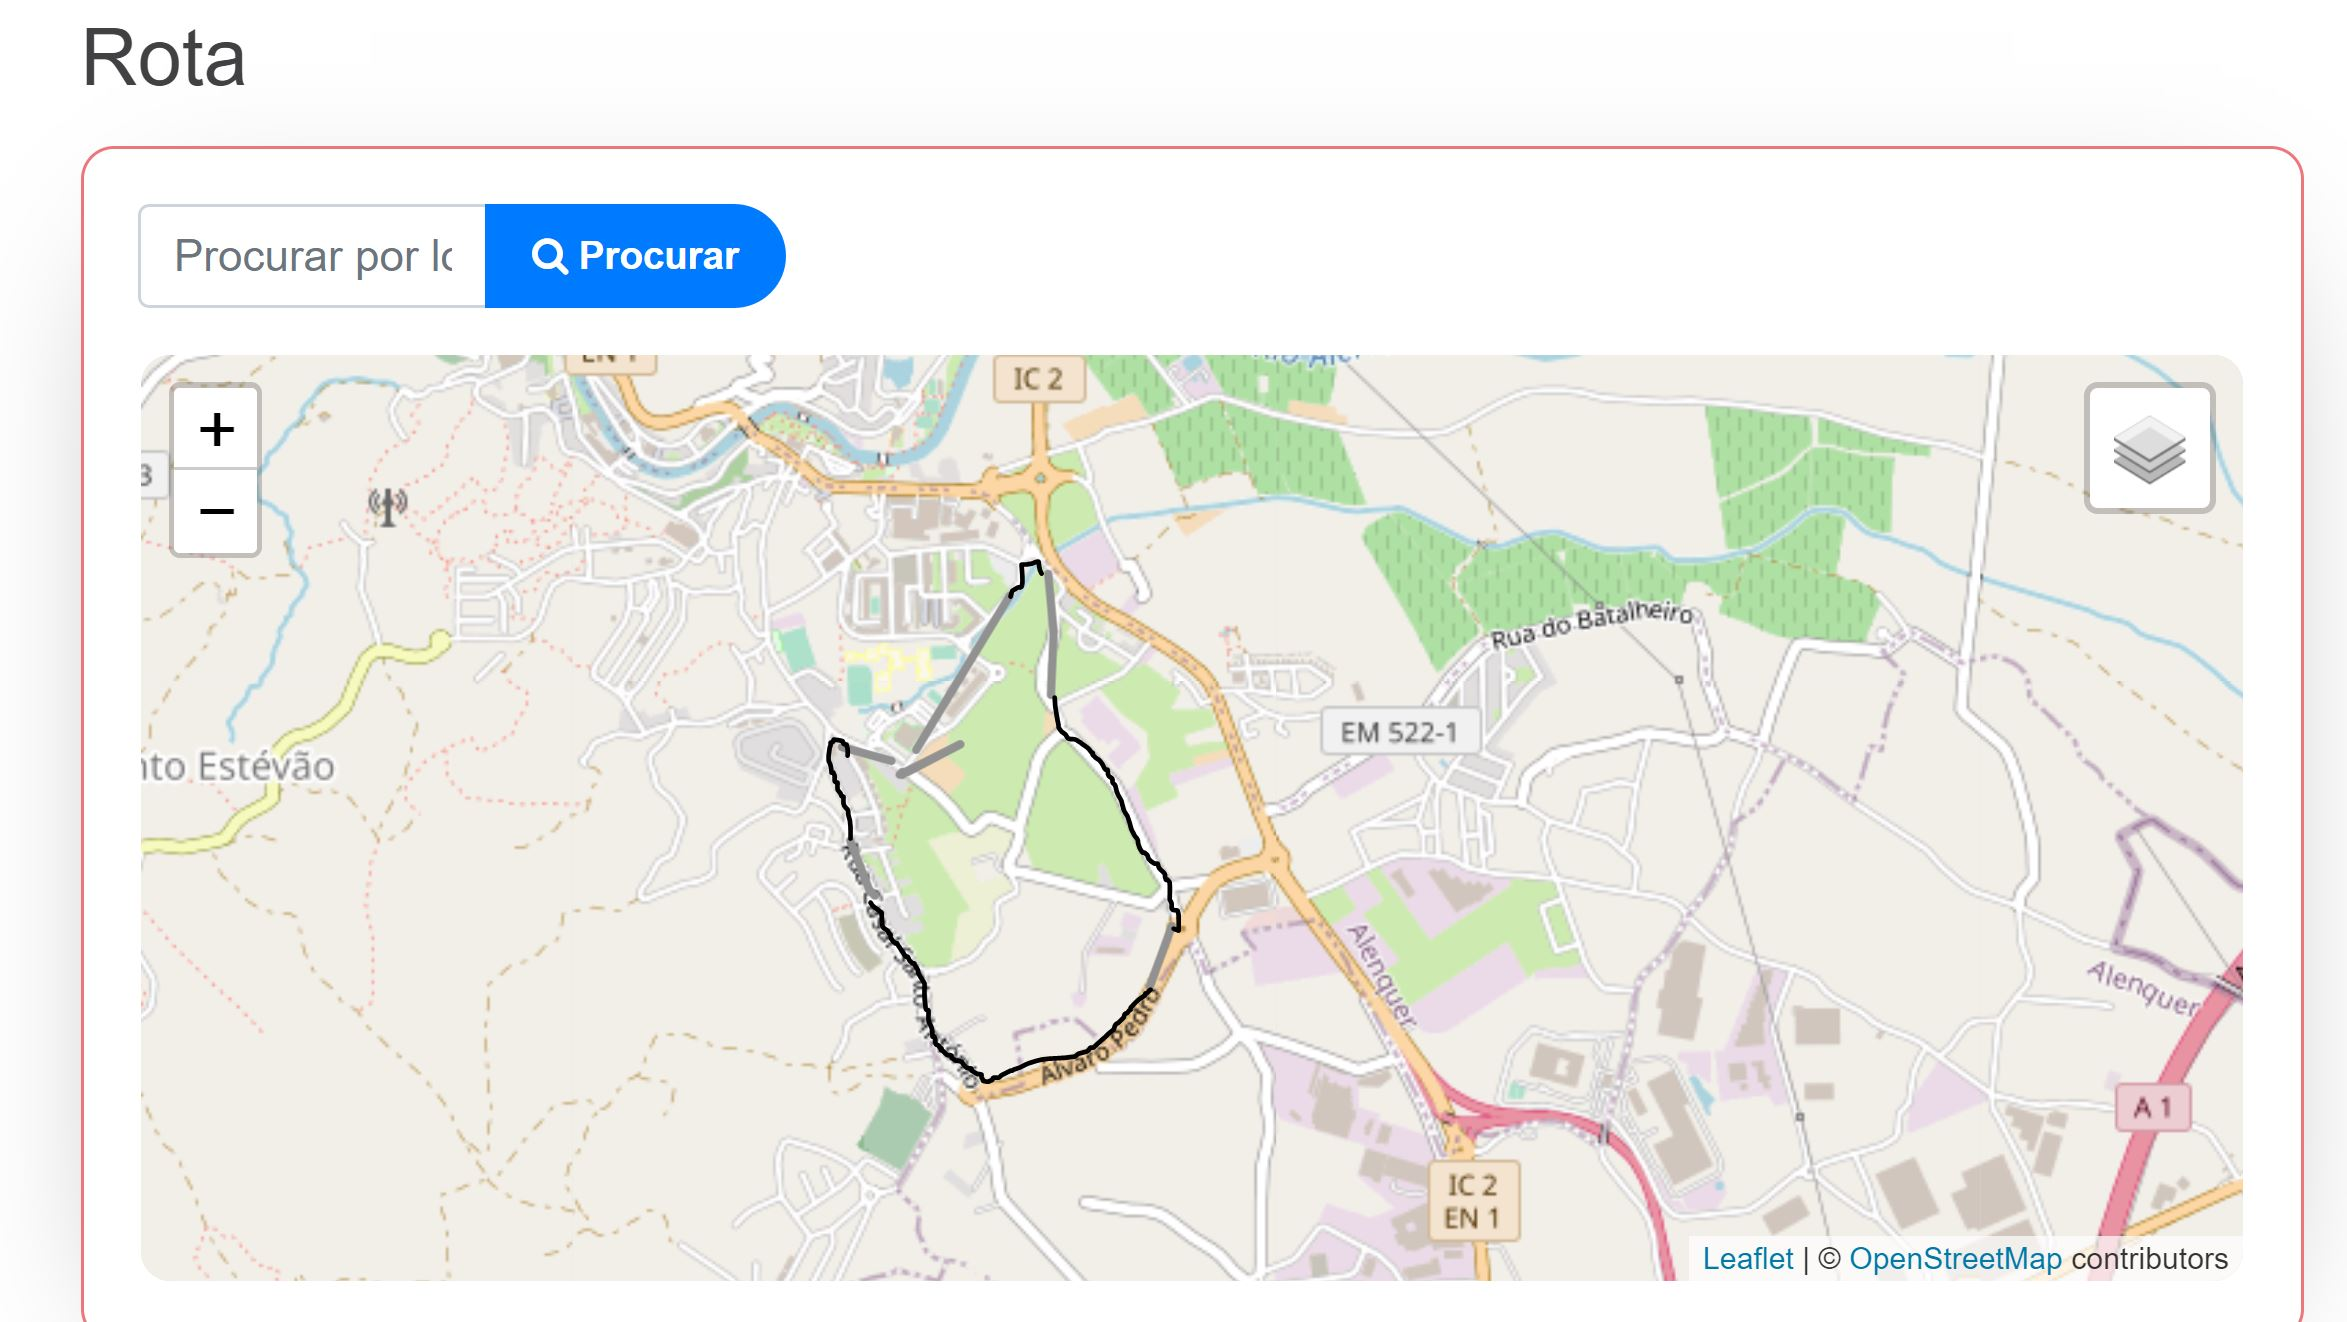
\includegraphics[width=0.5\linewidth]{Chapters/Figures/GPSREAL.JPG}}%
  \caption{GNSS Results}
  \label{fig:GNSS_Results}
\end{figure}

The next test consisted of defined a safe location area. Then cross to unsafe zone and acquire GNSS location. This location was done outdoor, at stationary speed. The device sent the location to the model as it is possible to observe in the first figure~\ref{fig:gpsnodered}, the model sent the information to the Carelink platform, which raised an SMS alert described in the middle figure~\ref{fig:sms}. Where there was a link to see the alert, as well as, the position of the patient, as shown in the figure~\ref{fig:web_Alert}. The combination of these three figures~\ref{fig:Unsafe Zone Alert} is the workflow behind an Unsafe zone Alert, here described working with GNSS location.\newline\newline

\begin{figure}[htbp]
  \centering
  \subcaptionbox{GPS Node Red \label{fig:gpsnodered}}%
    {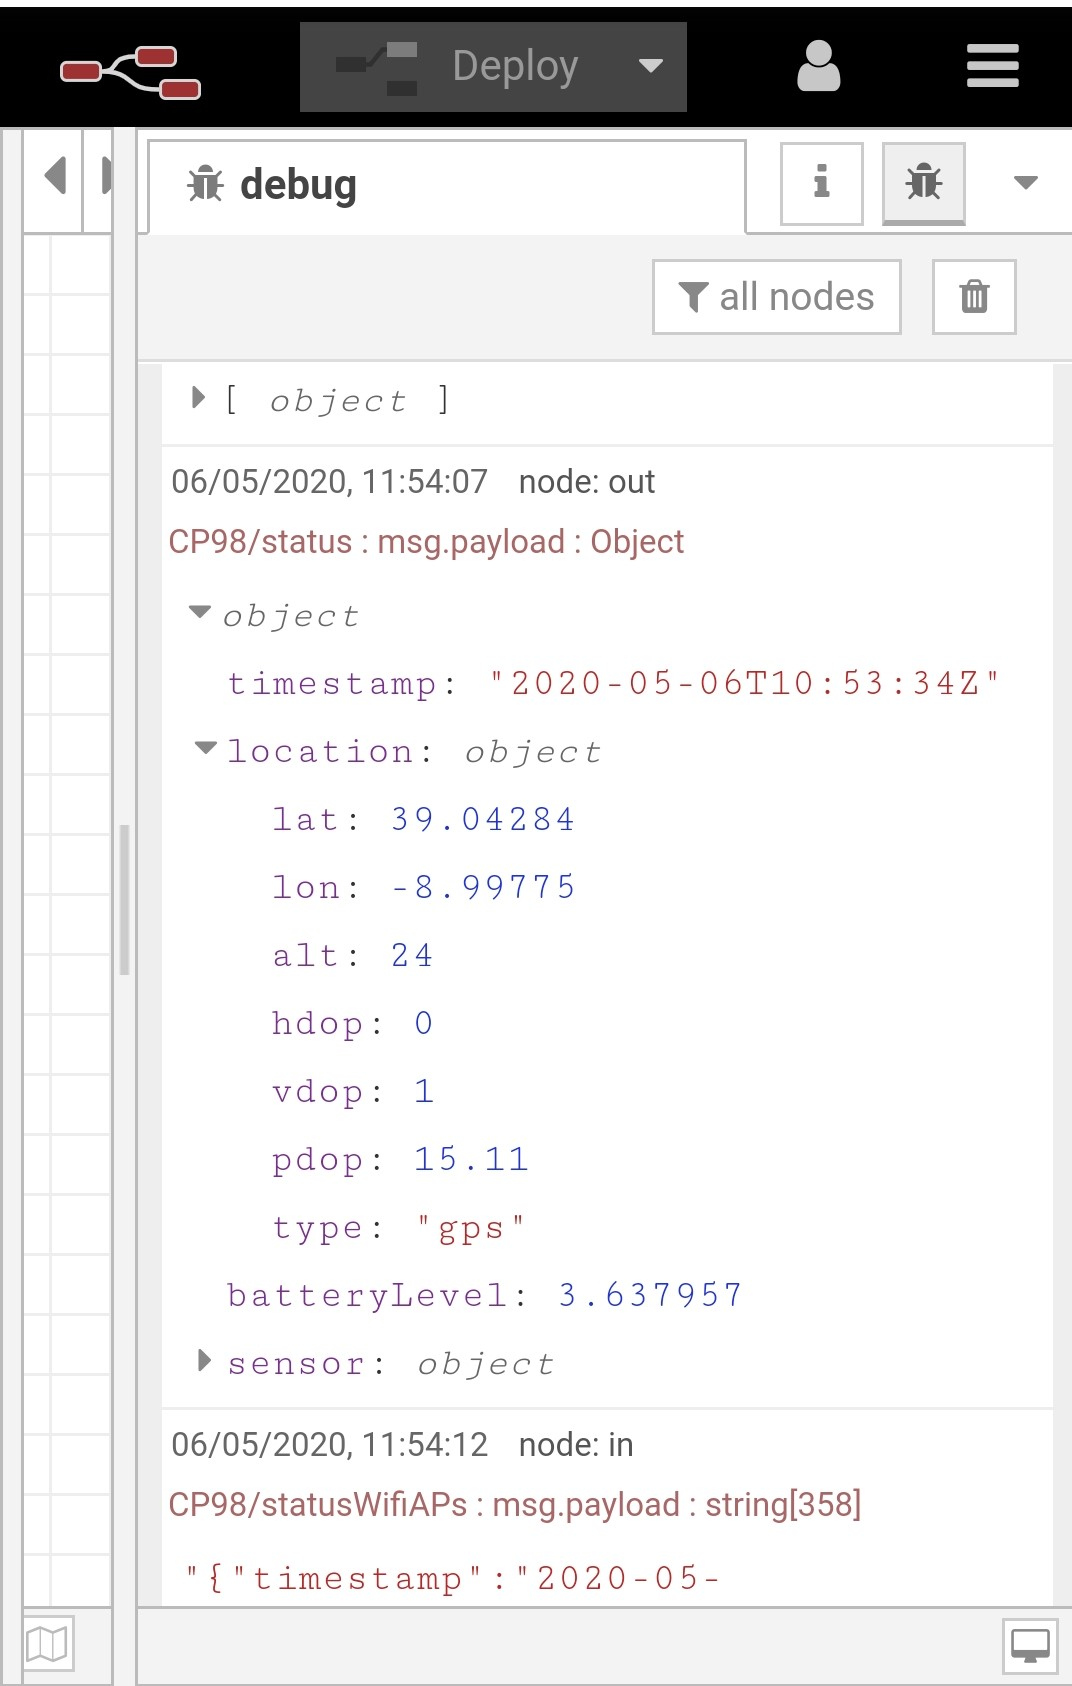
\includegraphics[height=8cm,width=0.3\linewidth]{Chapters/Figures/gpsnodered.jpg}}%
  \subcaptionbox{SMS Alert\label{fig:sms}}%
    {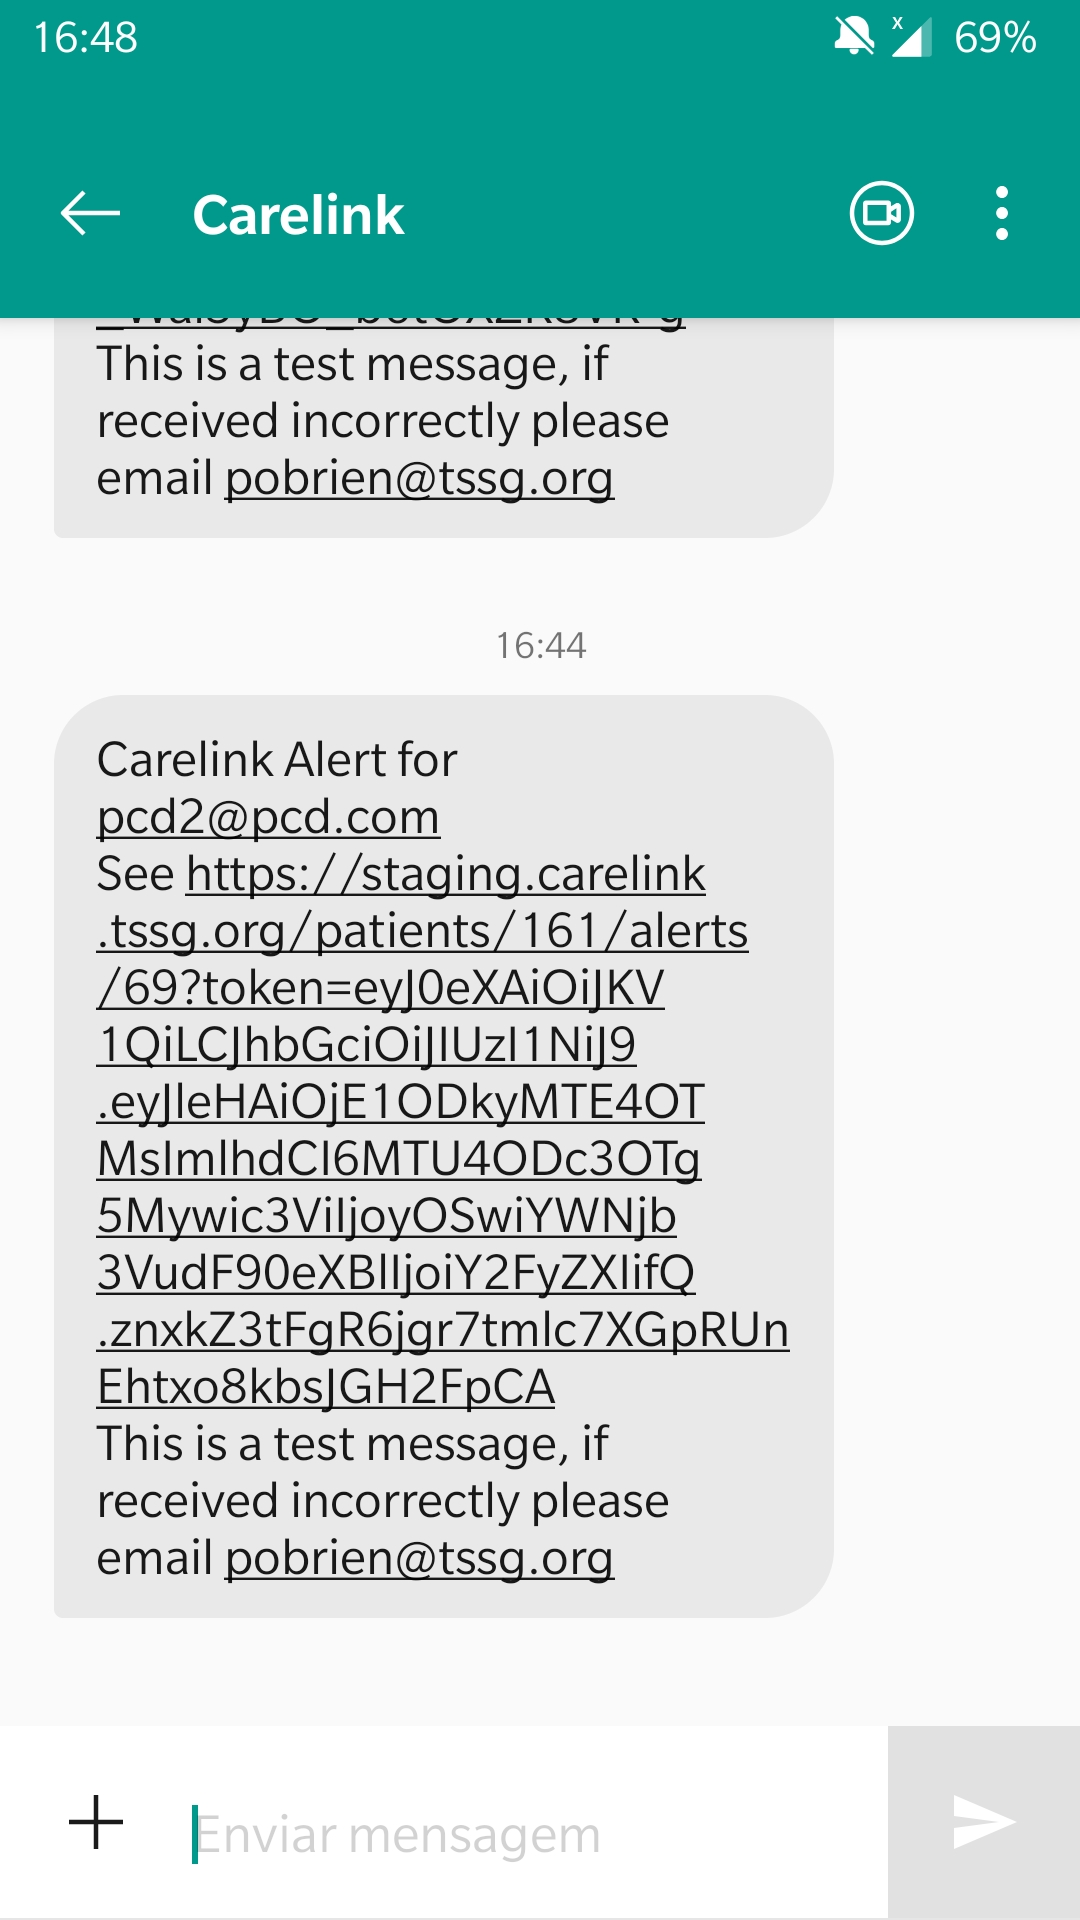
\includegraphics[height=8cm,width=0.3\linewidth]{Chapters/Figures/smsalert.jpg}}%
    \subcaptionbox{Web Alert\label{fig:web_Alert}}%
    {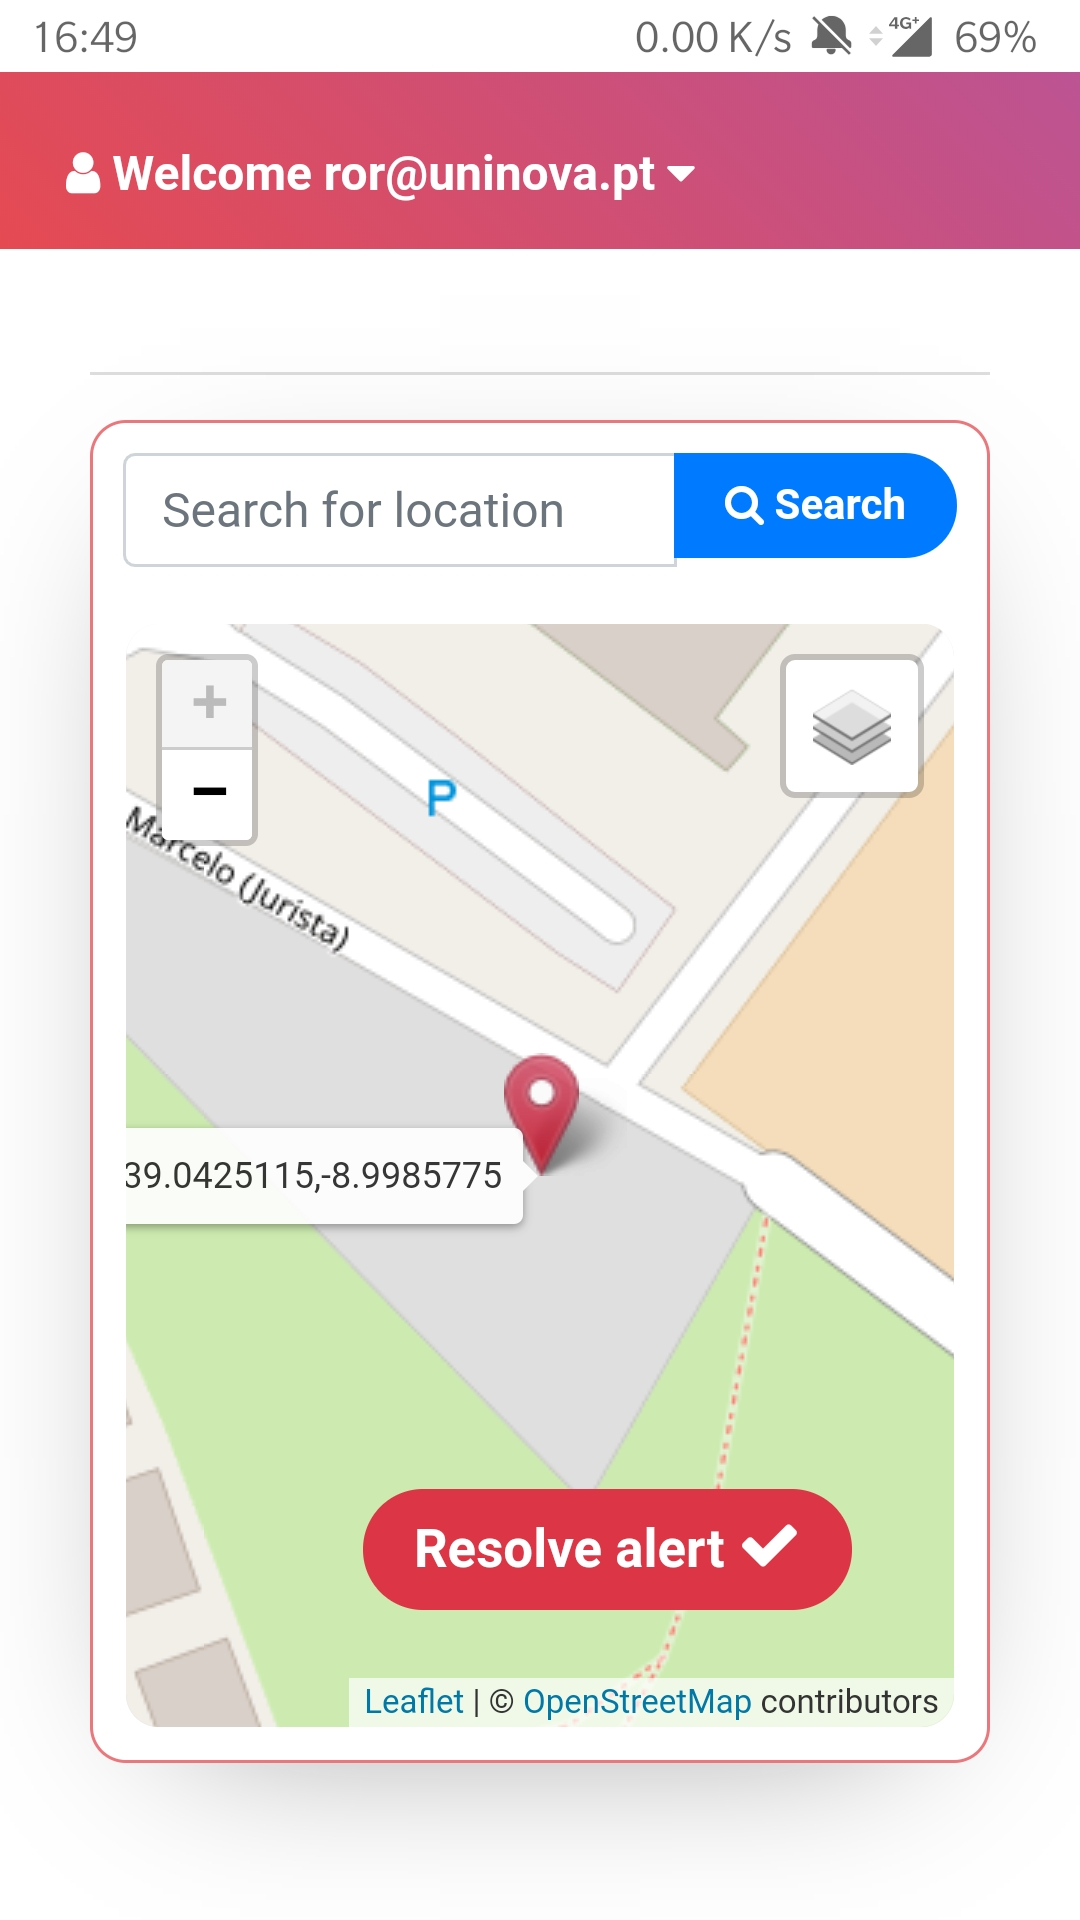
\includegraphics[height=8cm,width=0.3\linewidth]{Chapters/Figures/webalert.jpg}}%
  \caption{Unsafe Zone Alert }
  \label{fig:Unsafe Zone Alert}
\end{figure}

The location accuracy was from ($<2,5 to 11$) 5 m to 20 m. The time used to retrieve the location was approximately $120$ seconds after a cold start, and later it was immediate.

%###########################################
\subsubsection{WiFi}
\label{subsubsec:WiFi}
For the WiFi assisted location test was used the same material as above. The test had the same objective, that was simulating a patient walking. The test was conducted outdoor. And it was different from the previous scenario, because the communication used  was NB-IoT, allowing more mobility and a bigger range for the walking.

The test consisted in using the WiFi passive scanning principle, to discover WiFi access points,this information was then used to do the  assisted Location during walking, the average speed was 5km/h. 

The result of using the device in an urban route is possible to observe in the next figure~\ref{fig:WiFi_Results}, on the left side~\ref{fig:wifi} is the registered GNSS path, and on the right is the real path~\ref{fig:wifi_Real}.  The walk lasts for 40 minutes with a 2.8 km distance (about 80 location points), in an urban environment. Comparing both figures is possible to observe that in the figure from the right, at bottom exist a residential area close to the green area, that was no problem for the WiFi assisted location, but  close to the other green area exist a sports hall with a WiFi network and school with no WiFi, so this method was inaccurate in this part of the walk. The optimal scenario for this assisted location will be urban outdoor, where it can achieve accuracies closer to GNSS.

\begin{figure}[htbp]
  \centering
  \subcaptionbox{WiFi path \label{fig:wifi}}%
    {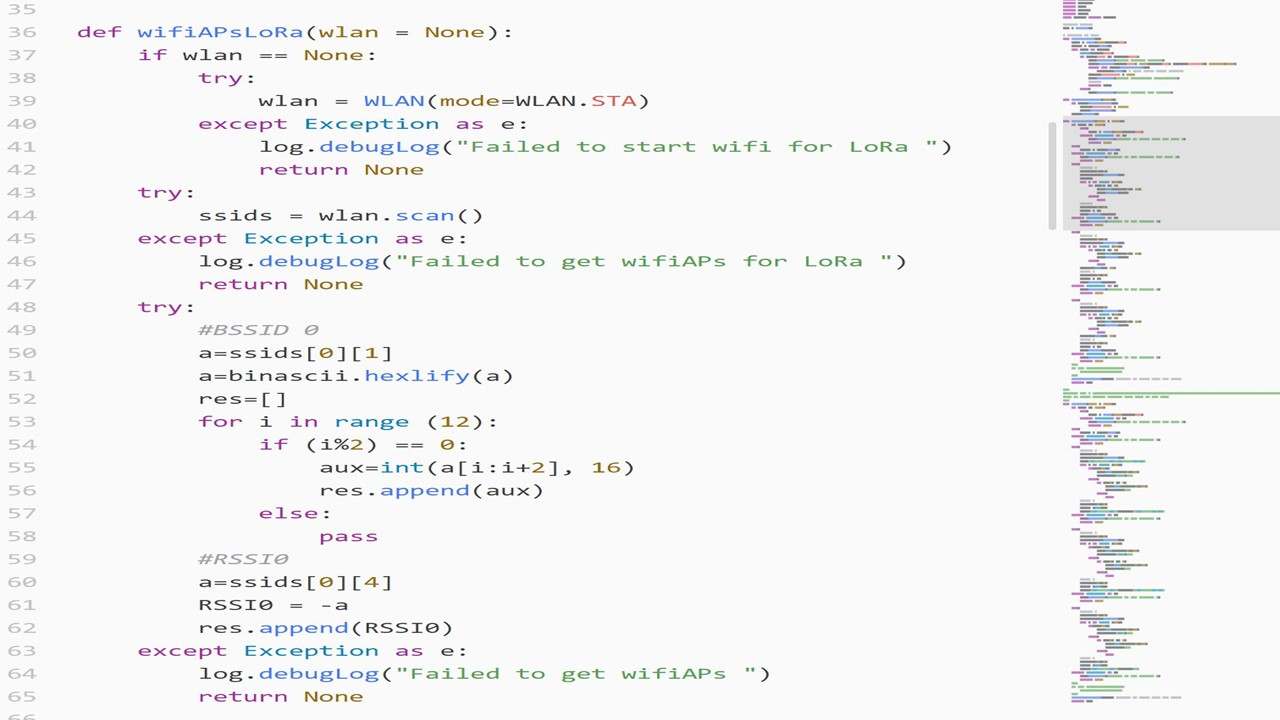
\includegraphics[width=0.5\linewidth]{Chapters/Figures/wifi.JPG}}%
  \subcaptionbox{Real path\label{fig:wifi_Real}}%
    {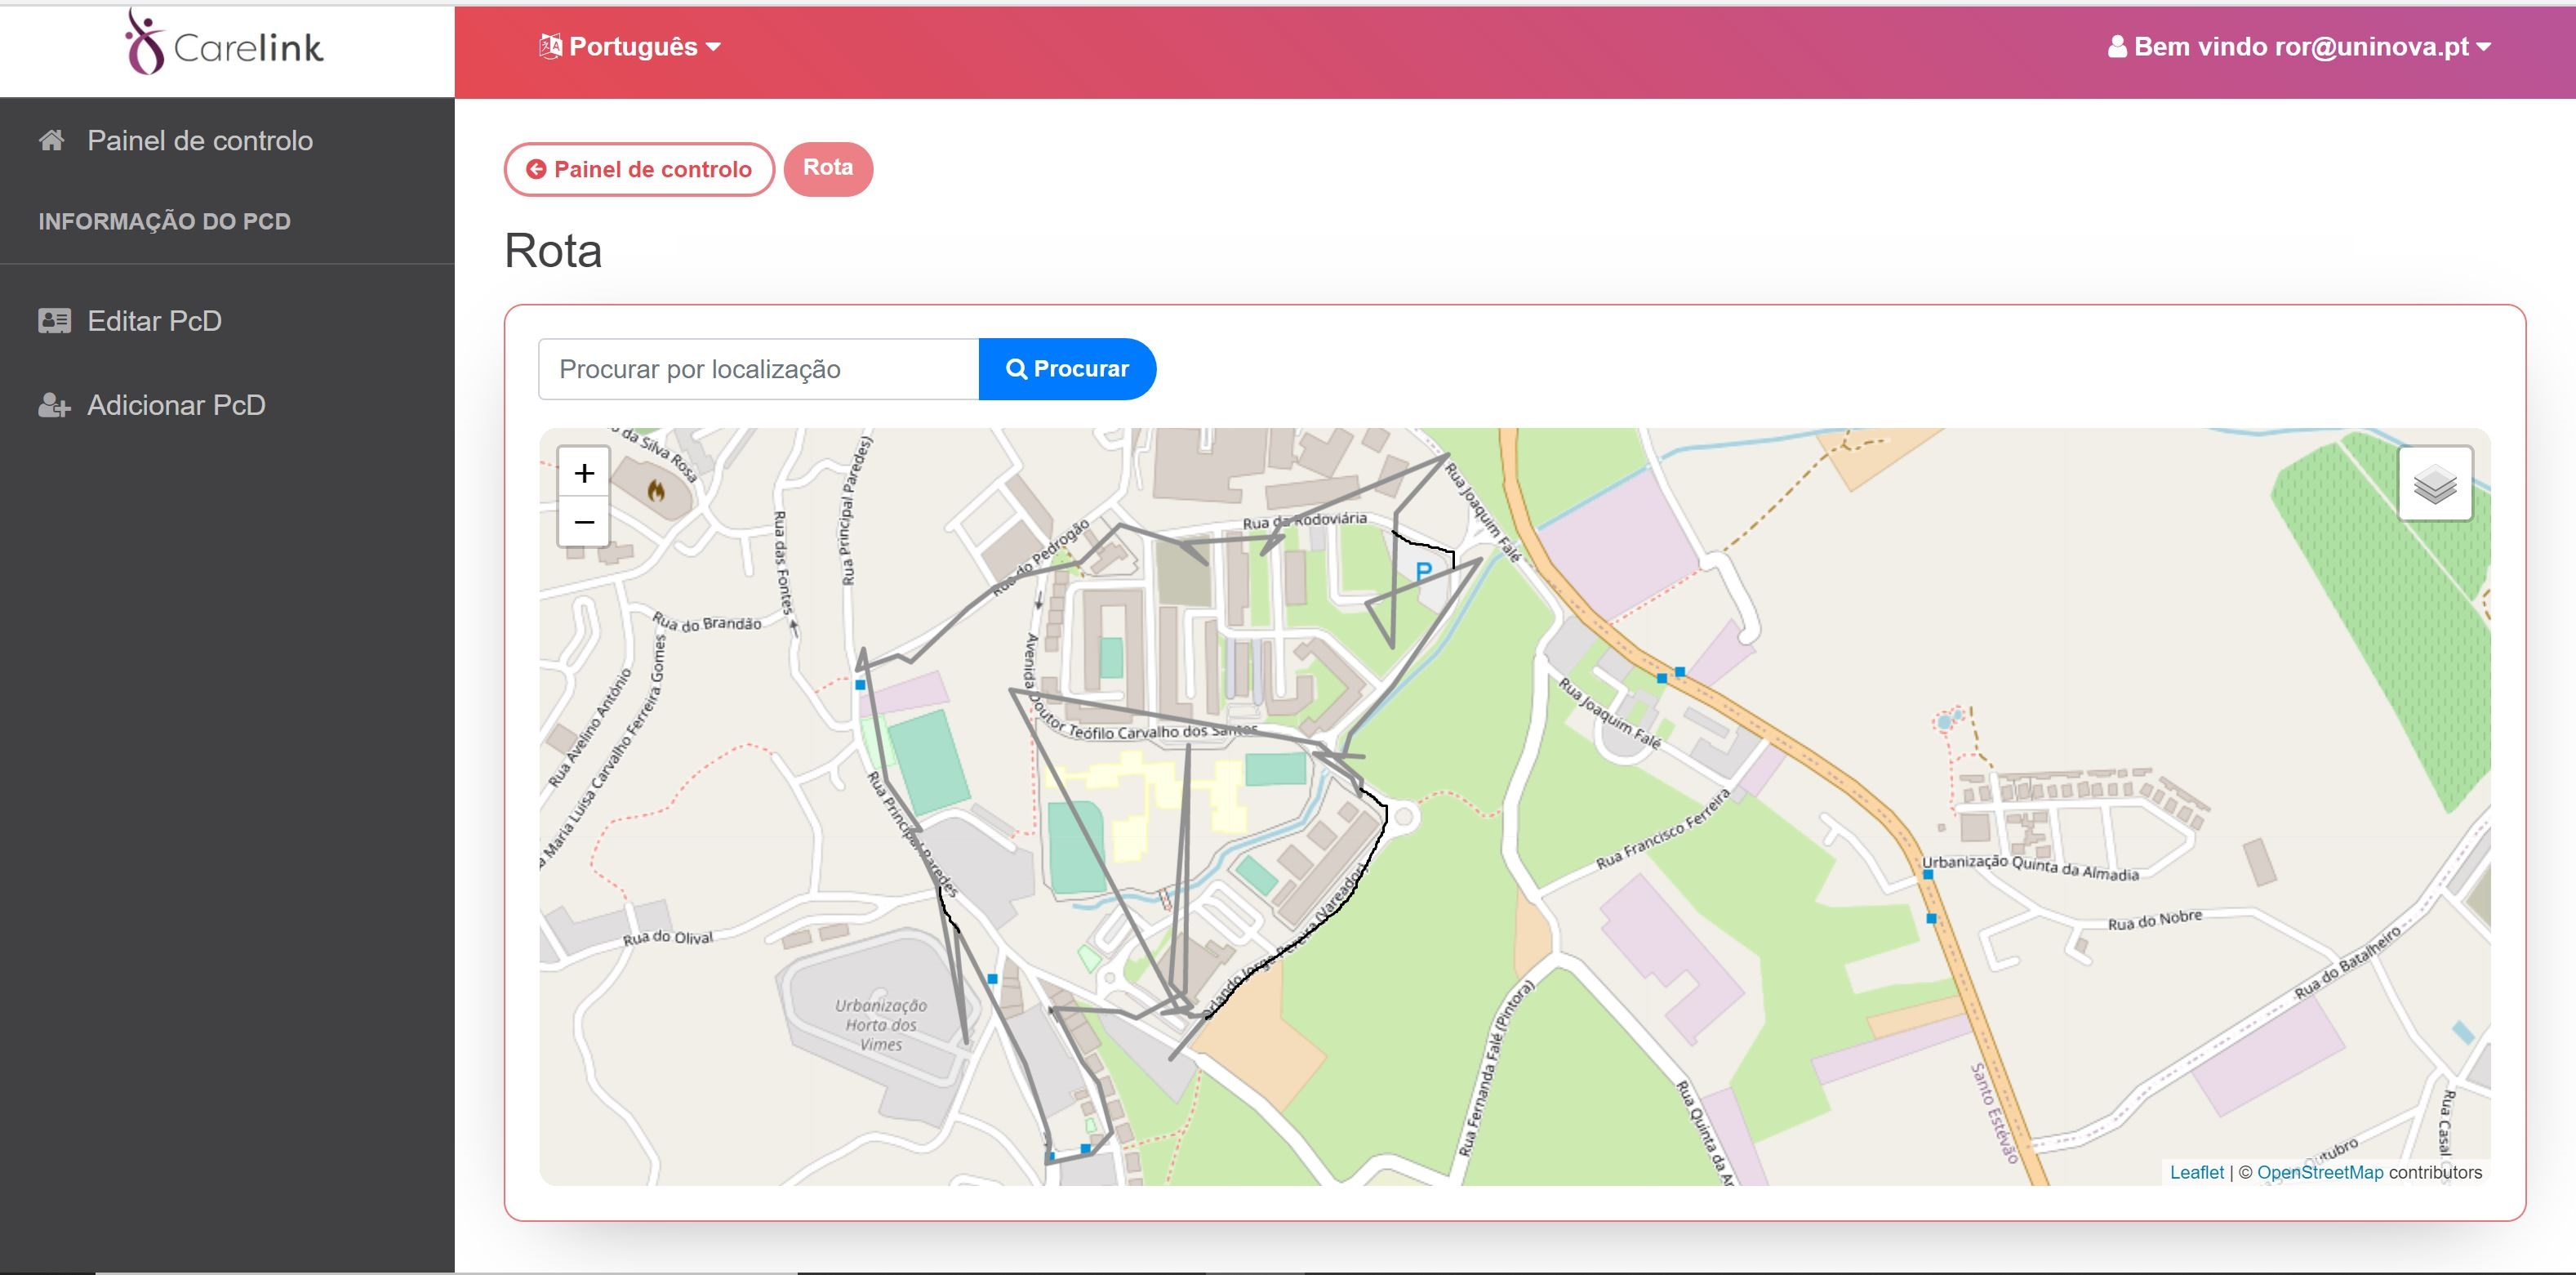
\includegraphics[width=0.5\linewidth]{Chapters/Figures/wifireal.JPG}}%
  \caption{WiFi }
  \label{fig:WiFi_Results}
\end{figure}

For this method to work, was used the same principle as above wherein the device side there was a scan for WiFi AP's. The device reads the  SSID, BSSID, RSSI.
After this generates an array and sent to the model. In the model, this array was converted to a JSON to construct a request for the three used API's (Google, Here, OpenCellID).
The API´s then returned the approximate location in different formats, these formats were standardized, and the most accurate one was chosen and sent to the platform,  as it is possible to observe in the figure~\ref{fig:wifi}.
The returned location accuracy is from  15m to 200m. The time used to retrieve the location was approximately $3$ sec. 

%"The median over 80 points was $x39$ meters with a standard deviation of $x21.63$ meters... " 

%#################################################################
\subsubsection{LoRa}
\label{subsubsec:LoRa}

The  LoRa Geolocation method was the last one tested. For this experiment was used the same FiPy. The LoRa antenna used was an external one ( molex ISM 105262, omnidirectional with 0.4 dBi Peak Gain at 868MHZ). In terms of software was used the LoRa Cloud (formerly Collos) API from Semtech, the TTN network server, and Cayenne~\cite{cayenne}.

The objective of the test consisted of using the Metadata present in the LoRa messages, to get an assisted location for one mobile FiPy, that was simulating the real patient. The test was a walk with a duration of 30 minutes, in an outdoor scenario, for a distance of 2km at an average walking speed of 5km/h. The result of using the device in an urban route is possible to observe in the next figure~\ref{fig:lora_geo_realpath}.

\begin{figure}[htbp]
  \centering
  
    {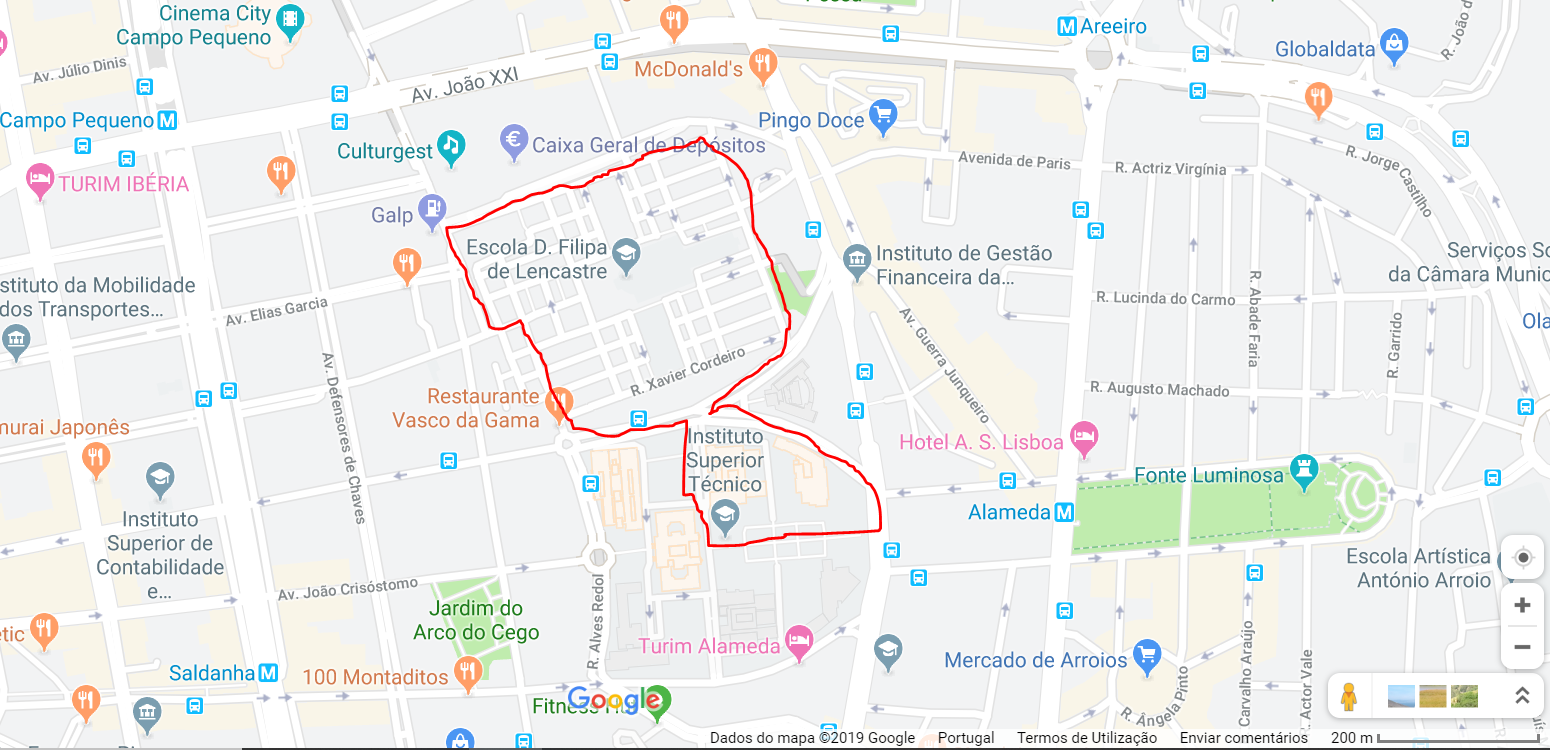
\includegraphics[width=0.8\linewidth]{Chapters/Figures/lorageorespercurso101019.PNG}}%
 
  \caption{LoRa Real path}
  \label{fig:lora_geo_realpath}
\end{figure}

The results of this test were dependent on the number of gateways in reach of the device, to perform the multilateration a minimum of three gateways were needed. So the location of the test was chosen taking on considerations this constrains, and one of the best places in Lisbon at the time of the test was the one from figure~\ref{fig:lora_geo_realpath}. For the Gateway were used three community gateways, with the objective to simulate a real usage scenario. From the data in figure~\ref{fig:lora_geo_GWs}, it can be seen that all of them covered the test area which is represented in red. 

\begin{figure}[htbp]
  \centering
  
    {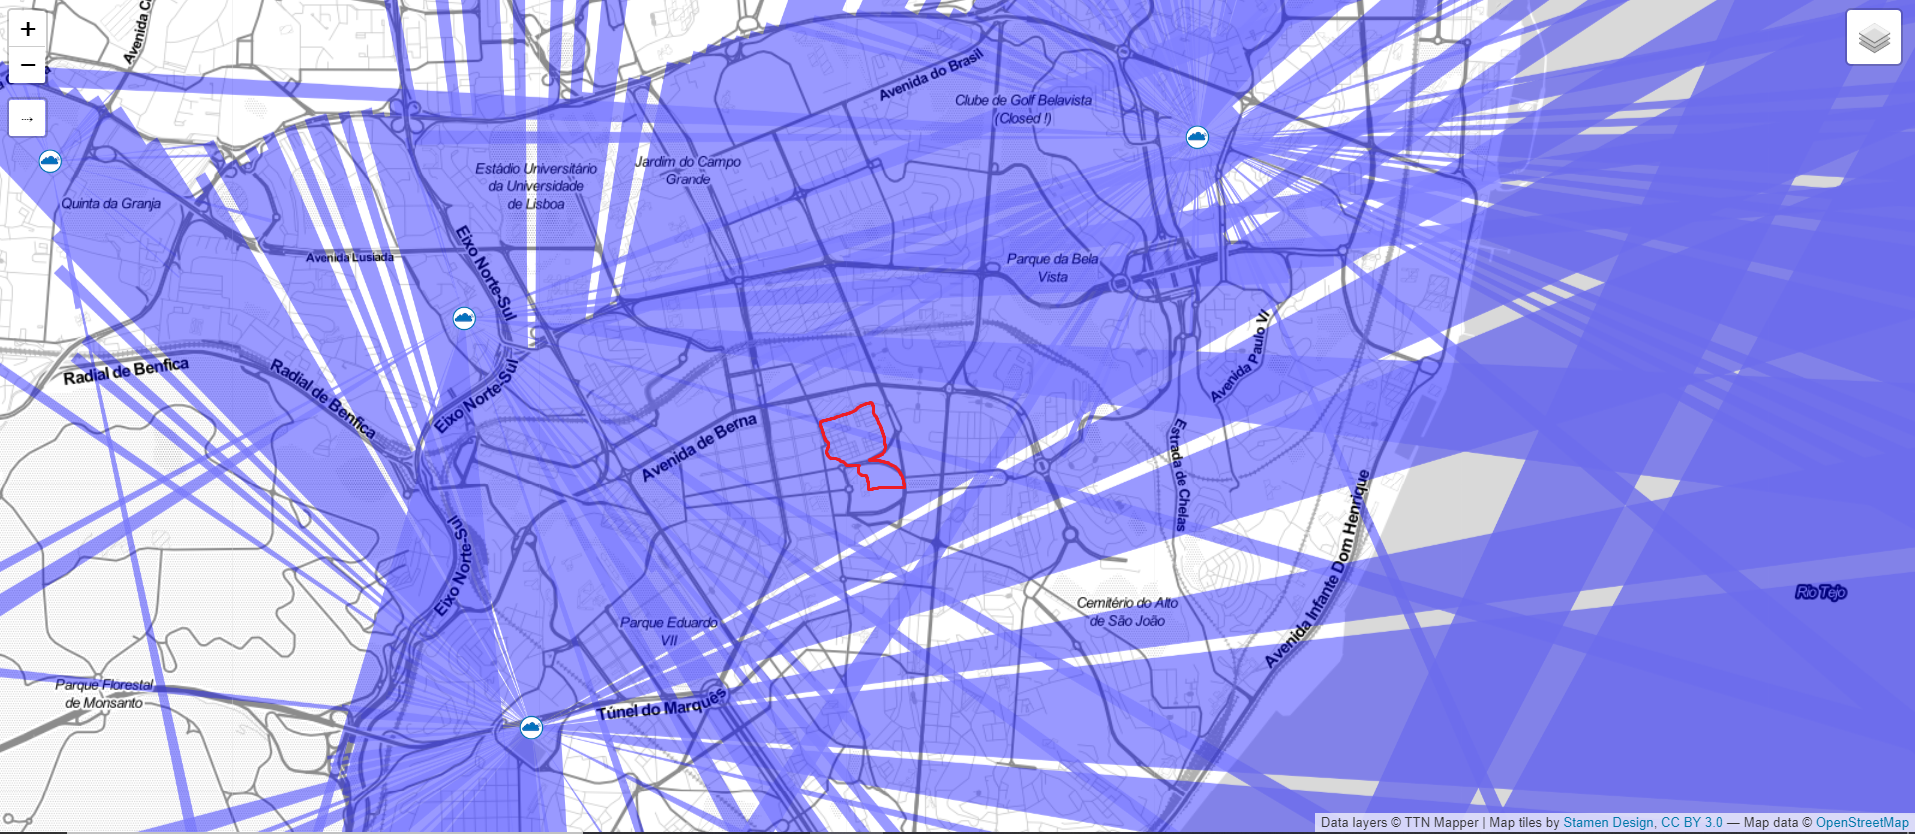
\includegraphics[width=0.8\linewidth]{Chapters/Figures/lorageoresttnmapperGWS.png}}%
 
  \caption{LoRa Gateways}
  \label{fig:lora_geo_GWs}
\end{figure}

The test was also conducted in an area central to all of the three gateways. The figure~\ref{fig:GW1LOS} shows the first one at a distance of 2.67 km. The second at figure~\ref{fig:GW2LOS} is at 2.85 km. The last in figure~\ref{fig:GW3LOS} was at 2.66 km. 

From these figures is possible to observe that none of the gateways had a direct line of sight. Although all of them were placed outdoor and possible on top of the buildings, it is possible, they had a line of sight, once the figures only represent terrain elevation and not building elevation. The first one is registered at 175m the second at 100m and the third is unknown, this information was from the TTN~\cite{TTN} and it was set by the owner of the gateways.

\begin{figure}[htbp]
  \centering
       {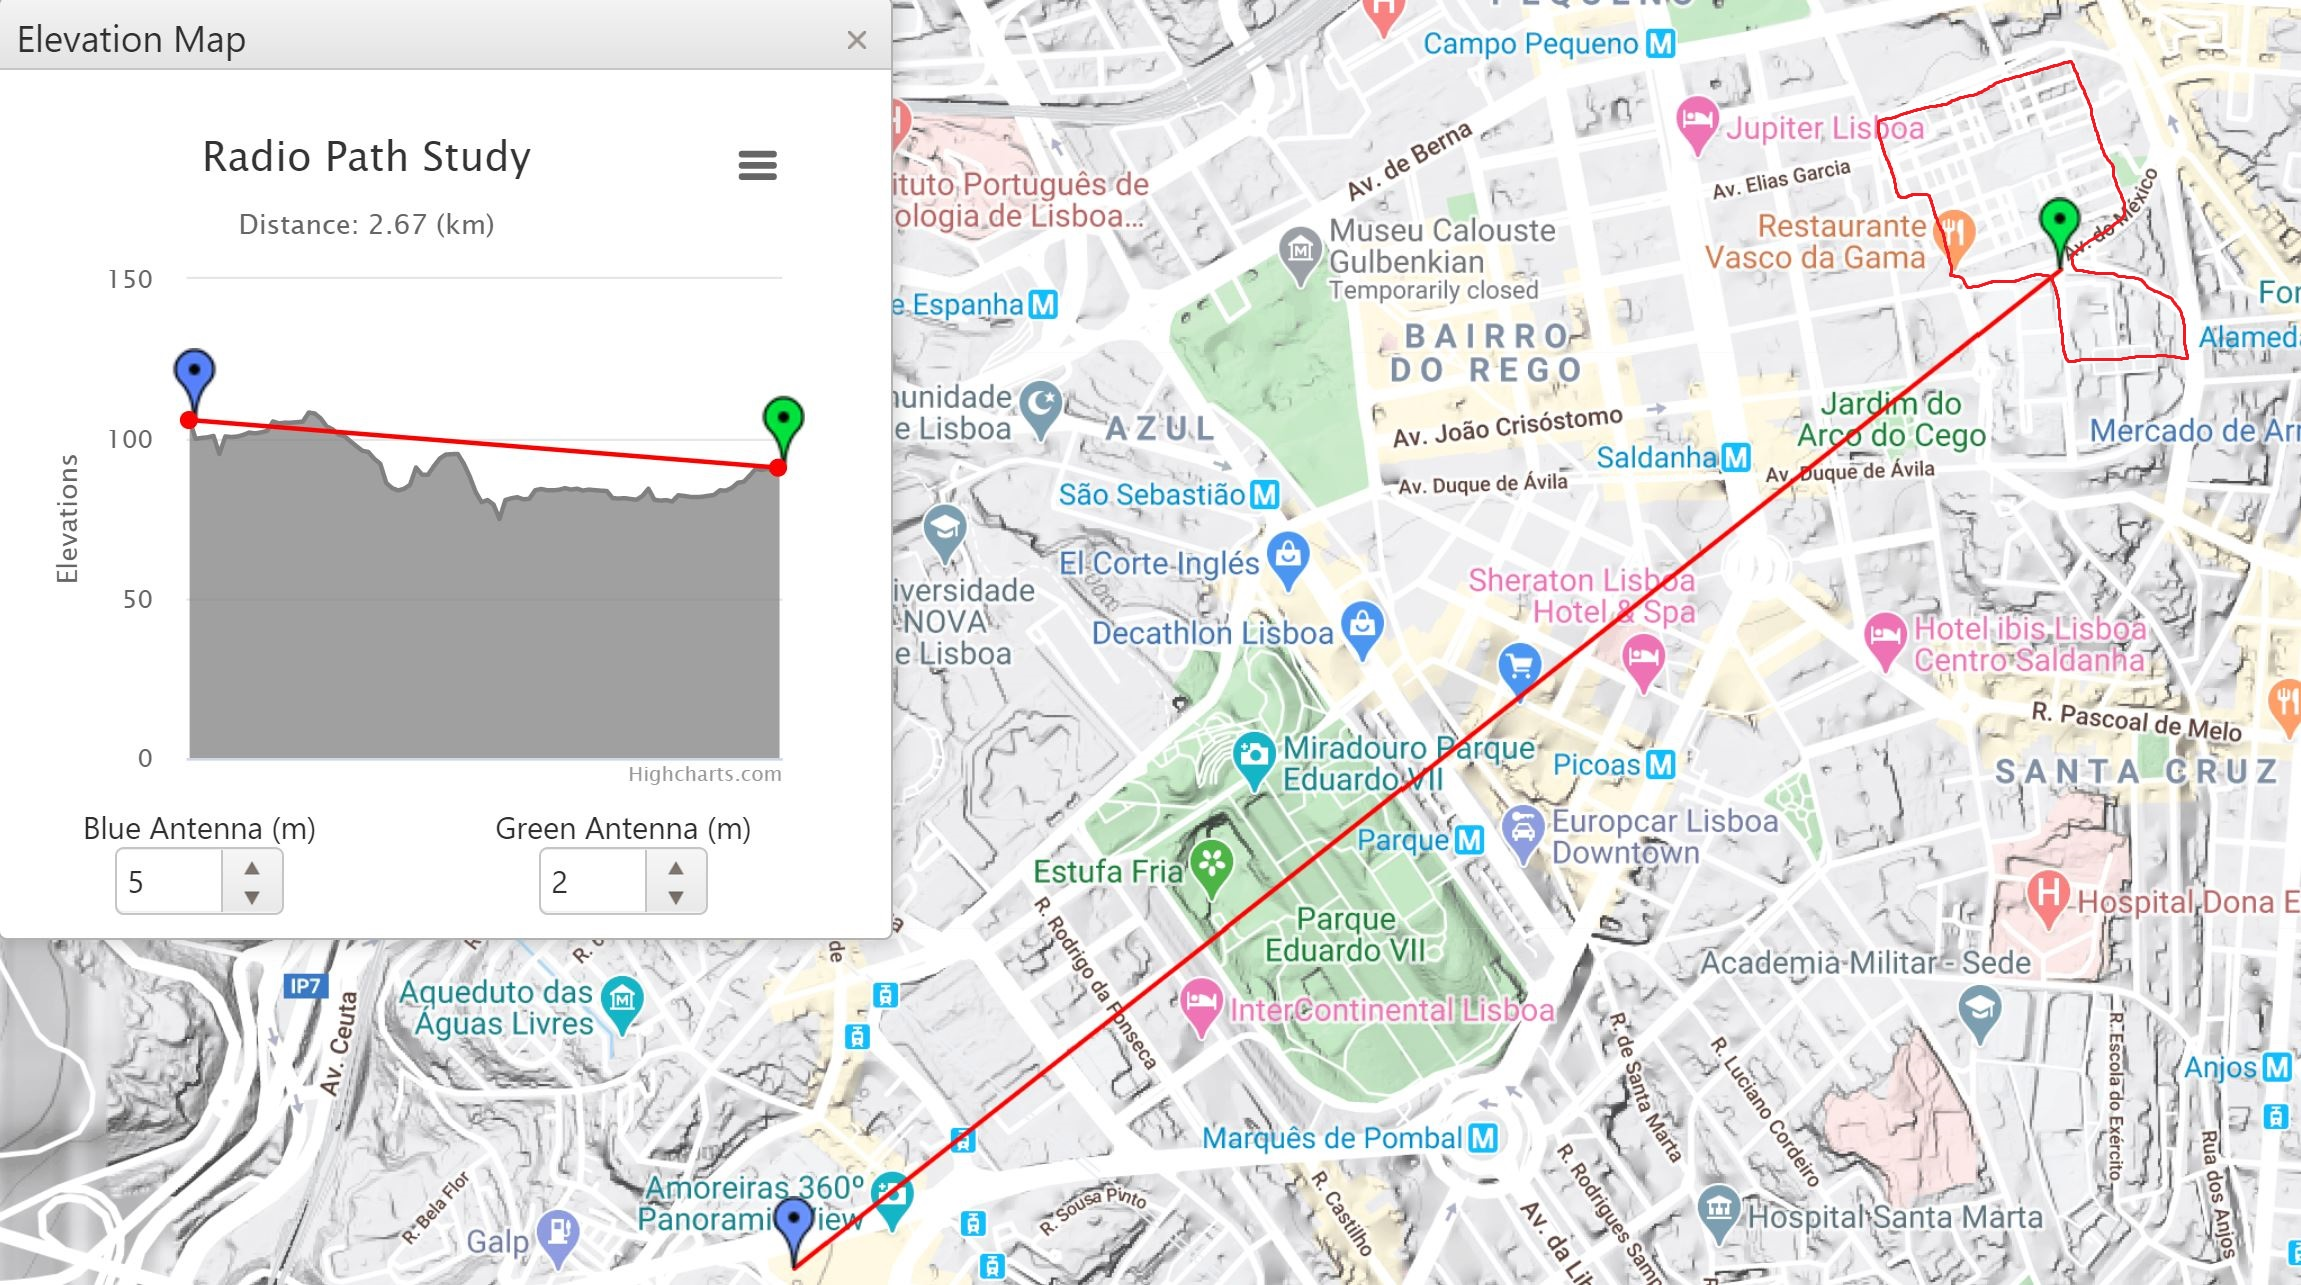
\includegraphics[width=0.7\linewidth]{Chapters/Figures/GW1.JPG}}%
   \caption{GW1 Distance and Line of Sight}
  \label{fig:GW1LOS}
\end{figure}

From the previous information was possible to expect, a concentration of points closer to the first gateway, since is the closer one with the better chances for a line of sight. 
\begin{figure}[htbp]
  \centering
      {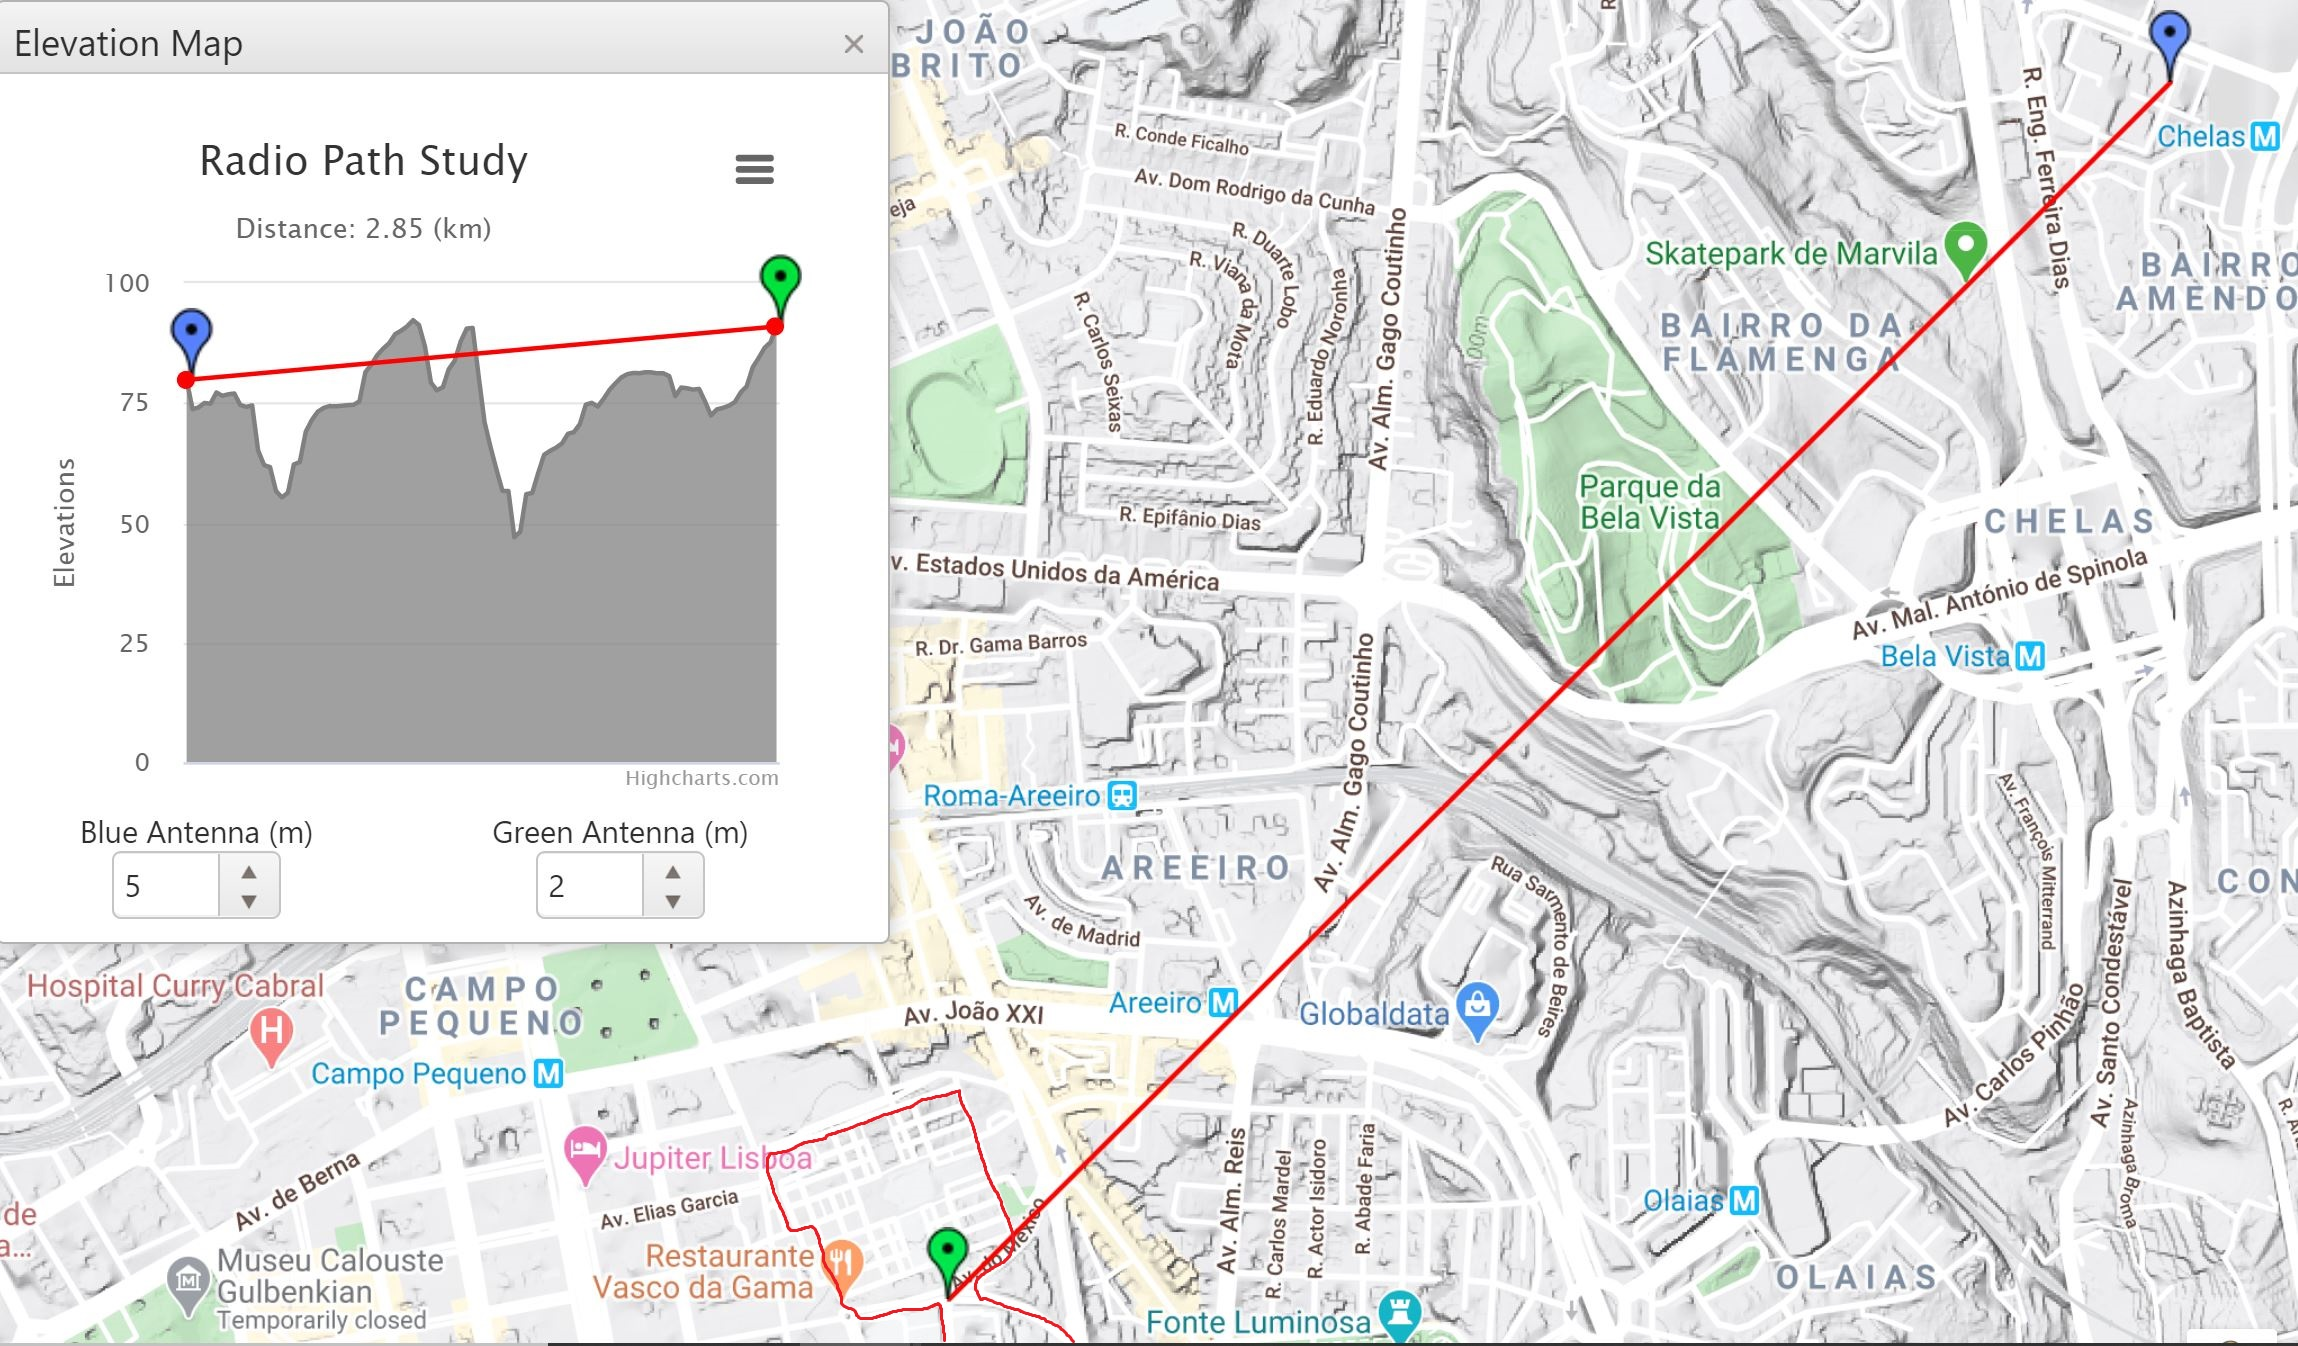
\includegraphics[width=0.7\linewidth]{Chapters/Figures/GW2.JPG}}%
  \caption{GW2 Distance and Line of Sight}
    \label{fig:GW2LOS}
\end{figure}

The third gateway should be the one with more difficulties to receive the packets. In device-side was sent the full payload. The configurations in use were the following: spreading factor 7, bandwidth 125 kHz, the first channels in 868.1 MHz, the coding rate at 4/5, the LoRa class as C and a Transmission power of 14 dBm. The use of  other specifications could result in other results, or using the adaptive data rate to change the Spreading factor could result in better reception from the gateways, but these specifications are the most common one from low-end gateways, and this test tried to replicate the normal usage from a patient anywhere in the world.

\begin{figure}[htbp]
  \centering
 {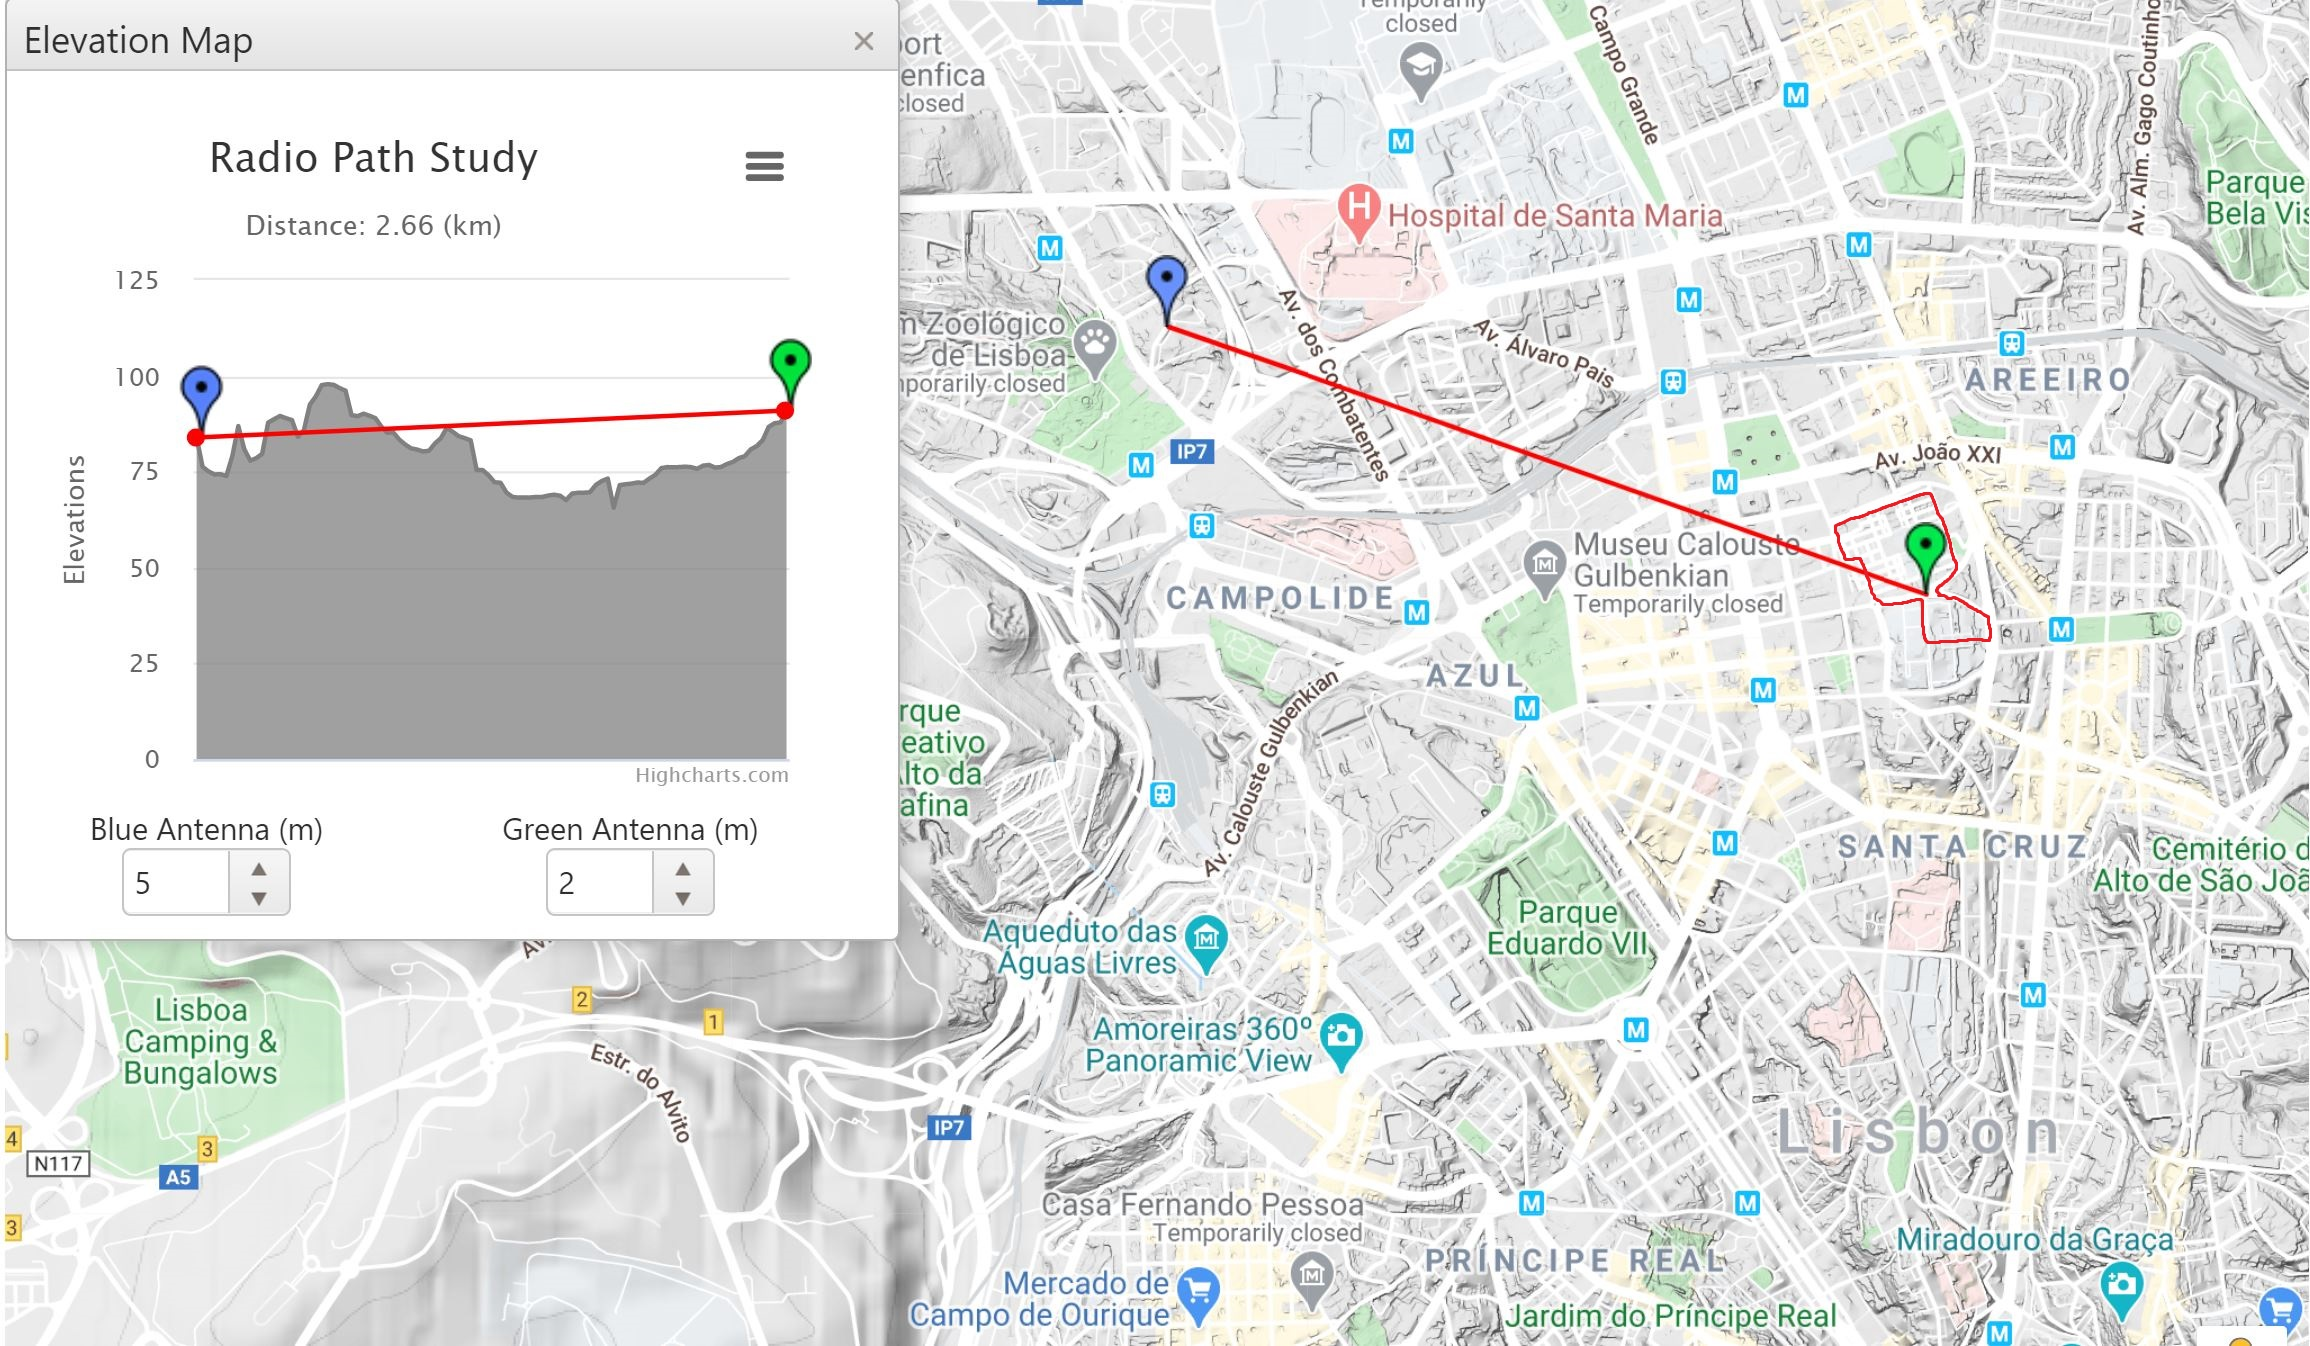
\includegraphics[width=0.7\linewidth]{Chapters/Figures/GW3.JPG}}%
   \caption{GW3 Distance and Line of Sight}
  \label{fig:GW3LOS}
\end{figure}

In the gateway side was simple a packet forwarded to the TTN server, the gateway added the Metadata to the message. In the TTN server was an integration with the LoRacloud API.
  
  
%################# V1 RSSI
The first result for the location is represented in the next figure~\ref{fig:lora_geo_res_rssiv1}, here is shown a map of all the locations points, this map was part of the Cayenne dashboard. In this dashboard, the blue circles represent a location from the device, the red line that is connecting the circles represent the route, and the blue balloon is the location of the device in a specific time, this time can be changed on the bottom slider.

For this first result was used the LoRacloud V1 single frame RSSI location. Which Calculates a location for a device according to RSSI data, received by the gateway. The property "Location" of the gateway was not required. However, this property can be used if the gateway and its antenna location were not provisioned in the system. This means that the location will be more accurate if the gateways have GNSS capabilities, or the location of them are accurately defined in the TTN.
 
\begin{figure}[htbp]
  \centering
  
    {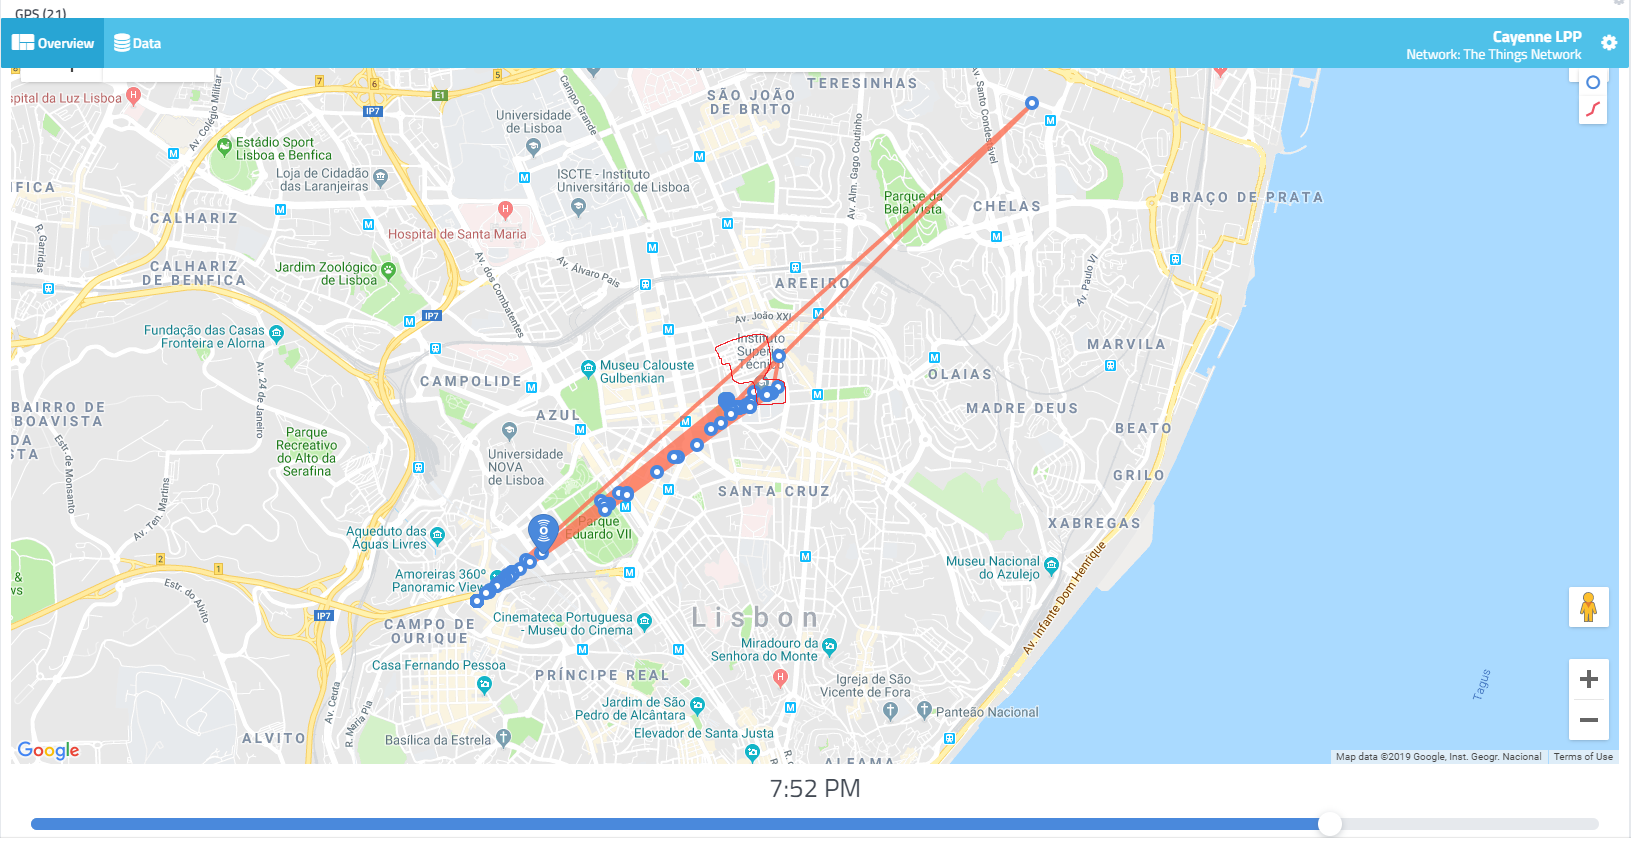
\includegraphics[width=0.8\linewidth]{Chapters/Figures/lorageores21-2.PNG}}%
 
  \caption{LoRa Location RSSI All points}
  \label{fig:lora_geo_res_rssiv1}
\end{figure}

In the figure~\ref{fig:lora_geo_res_rssiv1}, is possible to observe that the location points float within the Gateway 1 and 2, but are more close to the first this is caused by the fact the first one was receiving the messages with better RSSI, the factors for this can be a higher gain antenna on the receiver, better line of sight, or a multipath route for the test location. 

In The next picture~\ref{fig:lora_geo_res_RSSIV1_Zoom}, is shown a zoom of the test location, therefore removing all the others outliers, and it is possible to infer that some of the points are close to the real path (red line). The announced accuracy for this method previous stated in~\ref{fig:lora_Geo_compare} was 1000 to 2000 meters, and the observed was around 30 to 3000 meters.

\begin{figure}[htbp]
  \centering
  
    {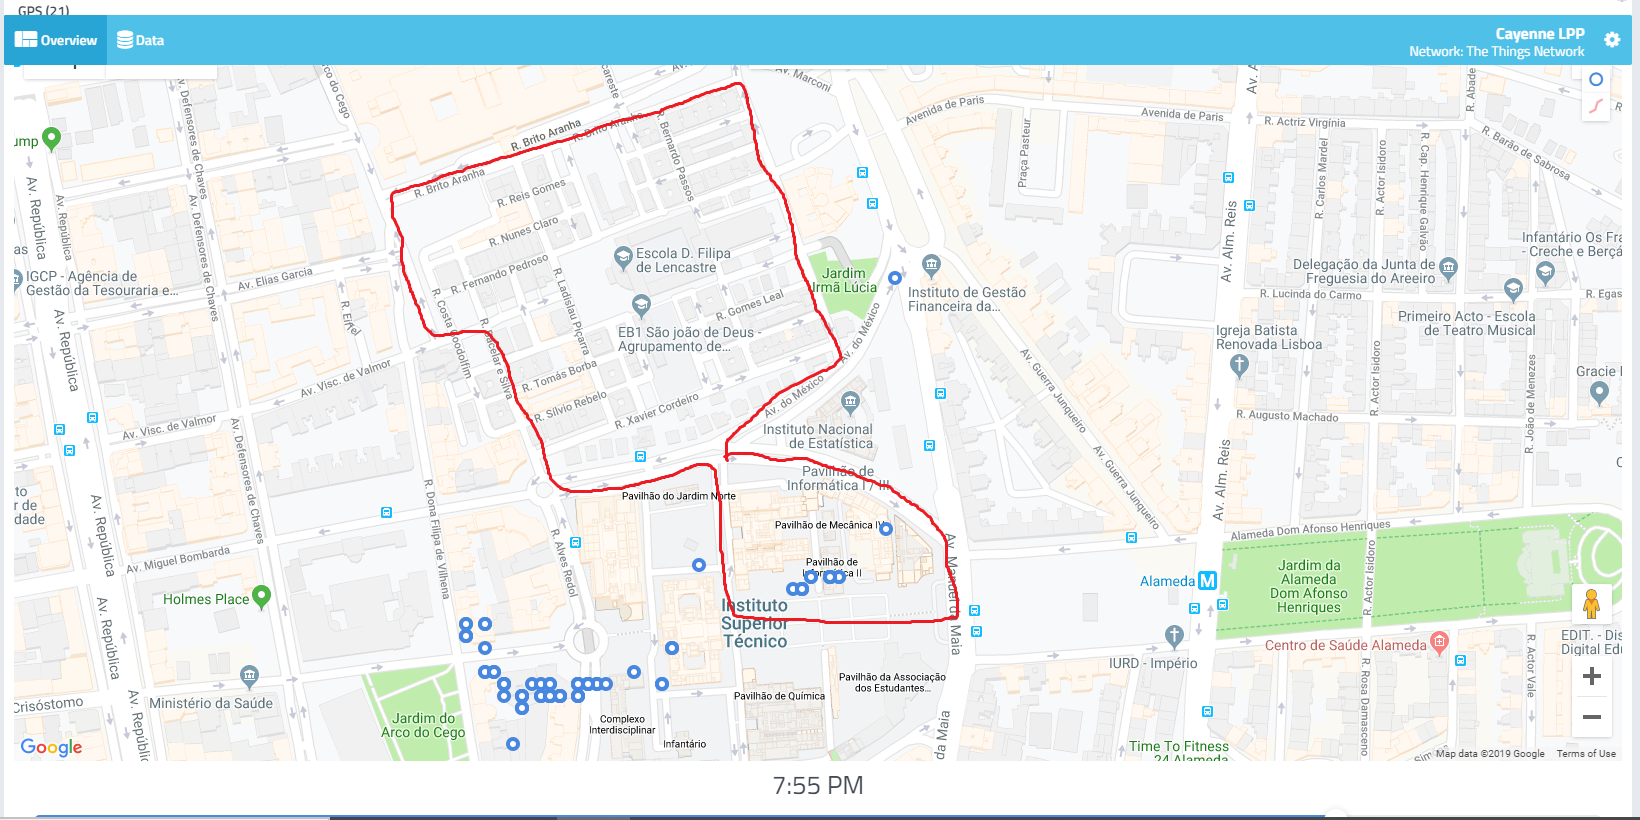
\includegraphics[width=0.8\linewidth]{Chapters/Figures/lorageores21-1.PNG}}%
 
  \caption{LoRa Location RSSI Zoom}
  \label{fig:lora_geo_res_RSSIV1_Zoom}
\end{figure}





%######################### V2 TDOA
For the second result was used the LoRa cloud V2 TDOA, which solves the location for the device according to RSSI Metadata combined with high-resolution time of arrival (TOA) Metadata. The time of arrival is measured in nano-seconds and is only supported by LoRa gateways with the necessary high-resolution time-stamping features, that are the ones with GNSS. The figure~\ref{fig:lora_geo_resTDOA1}, shows all of the points.
\begin{figure}[htbp]
  \centering
  
    {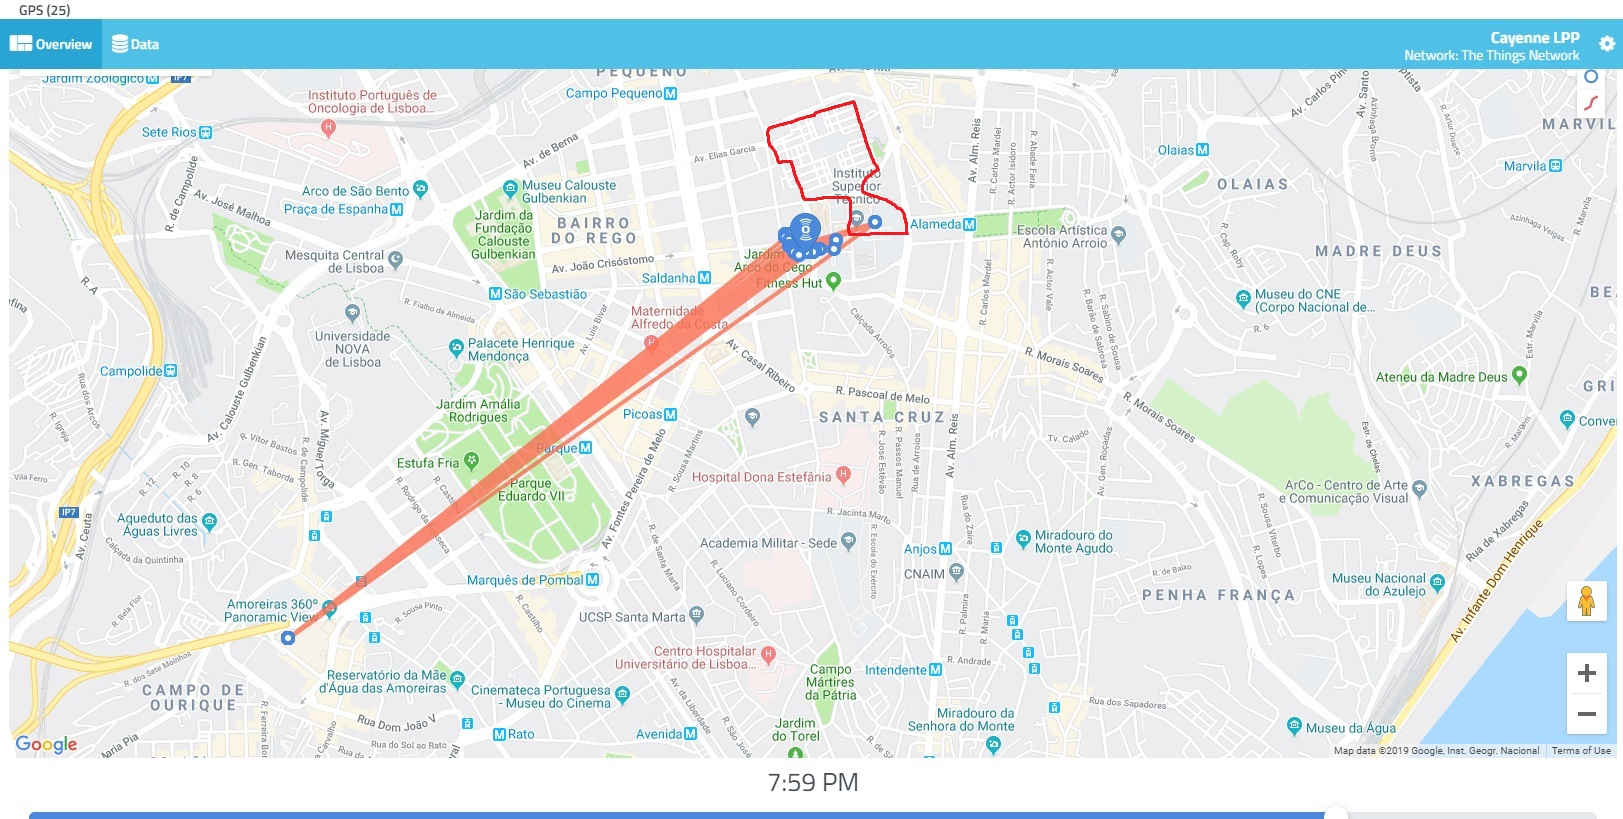
\includegraphics[width=0.8\linewidth]{Chapters/Figures/lorageores25-2.jpg}}%
 
  \caption{LoRa Location TDoA all pooints}
  \label{fig:lora_geo_resTDOA1}
\end{figure}

Concerning the previous method is possible to observe fewer outliers, and also fewer points when the zoom is done in figure~\ref{fig:lora_geo_resTDOAZOM}. This was possibly caused to the restrictions of having a high-resolution time-stamping, and perhaps only the gateway one had it or at least had the better time-stamping. The announced accuracy for this method was 20 to 200 meters, and if the gateway location point is considered an outlier the result was close, from 30m to 350m. Could have been improved maybe with other gateways, but comparing figure~\ref{fig:lora_geo_resTDOA1} with figure~\ref{fig:lora_geo_res_rssiv1} was an improvement.

\begin{figure}[htbp]
  \centering
  
    {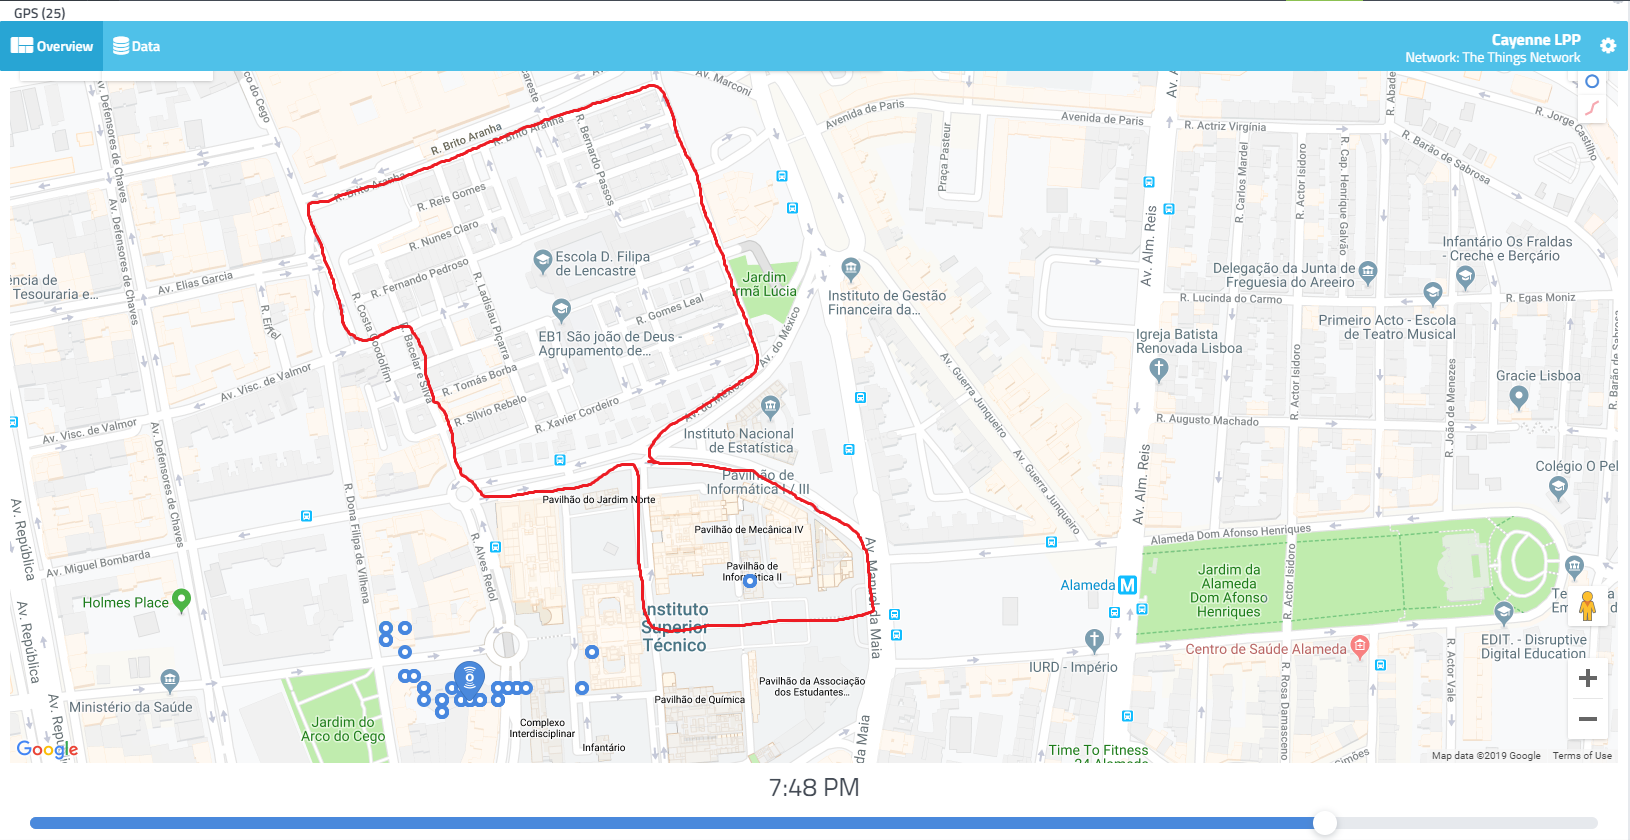
\includegraphics[width=0.8\linewidth]{Chapters/Figures/lorageores25-1.PNG}}%
 
  \caption{LoRa Location TDoA Zoom}
  \label{fig:lora_geo_resTDOAZOM}
\end{figure}






%####################V3
The last results were from LoRa cloud V3 Multiframe, this technique calculates the location for a device, according to the RSSI data captured from multiple LoRa frames (uplinks). This technique uses a sequence of single frames (consisting of multiple uplink objects), that are typically received by the gateways within a short time frame. These frames are assumed to be transmitted by the device in the same location. The result is a single location estimation.

Using the sequence of radio frames for a single estimation allows a location with higher accuracy than the single-frame alternative. The multi-frame technique also combines all the available data (RSSI, TDOA, SNR) into a single calculation. This results in a location estimation that is generally more accurate than do the average of multiple locations, that were calculated from several single frames.

This technique will work better with higher sample rates from the device, or with a stationary location. The following figure~\ref{fig:lora_geo_multiframe}, represents the location points for this method. Comparing to the previous method the results were almost the same due to the fact the locations were retrieved during walking and were not stationary, and the sample time of 30 seconds was maybe too high for getting multiple frames in the same location, or at least in a close enough location.
\begin{figure}[htbp]
  \centering
  
    {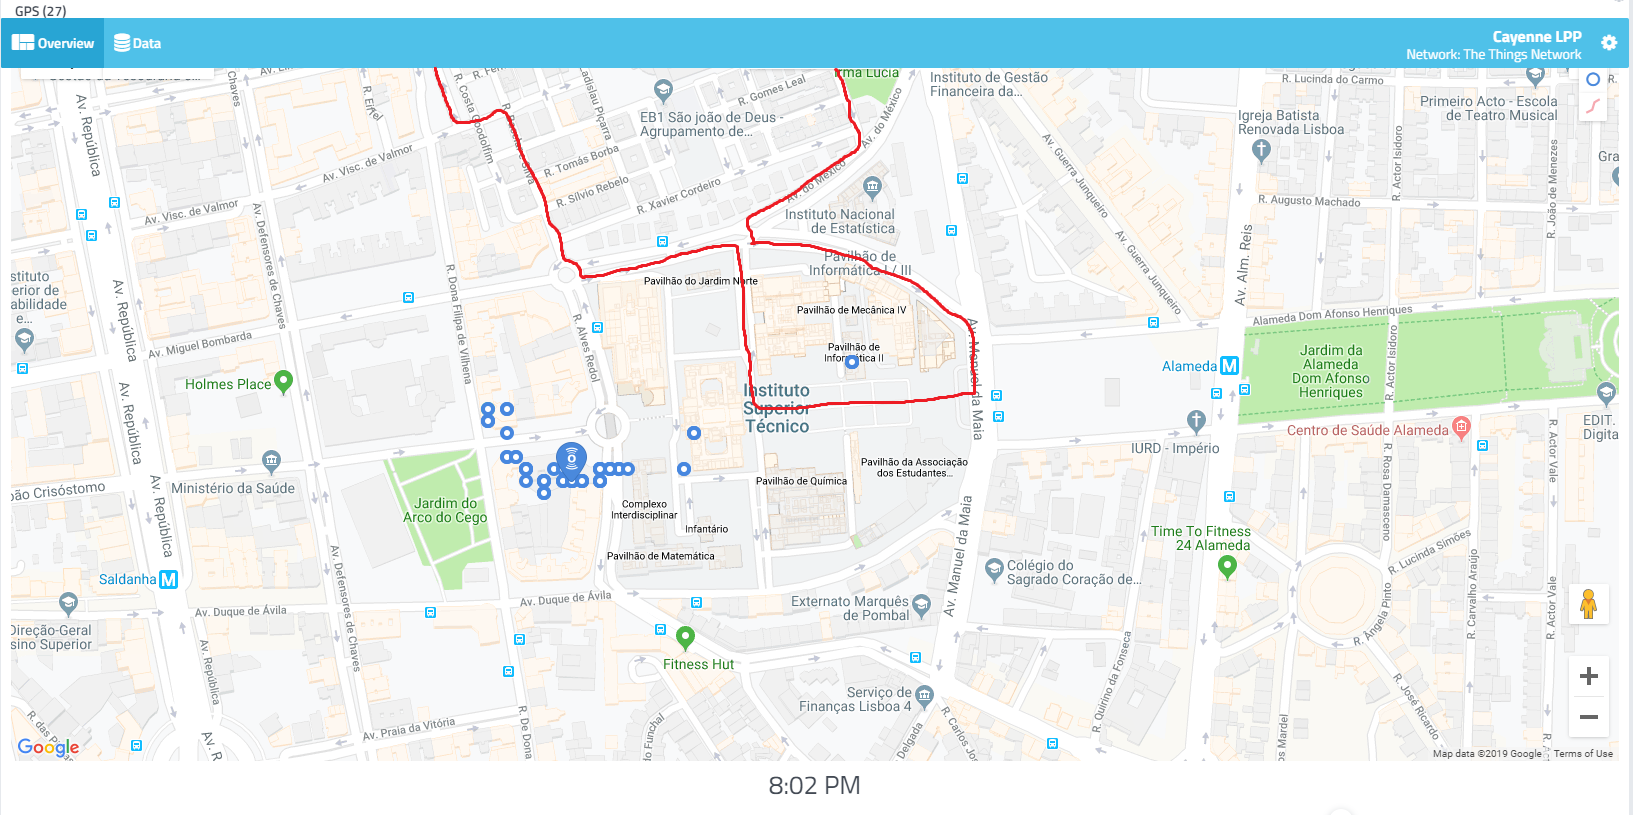
\includegraphics[width=0.8\linewidth]{Chapters/Figures/lorageores27-3.PNG}}%
 
  \caption{LoRa Location RSSI All points}
  \label{fig:lora_geo_multiframe}
\end{figure}


The returned location accuracy for the 3 methods was from  30 m to 3000 m. The time used to retrieve the location is approximately $2$ sec, and LoRa was used to transmit the Status message, although was not the full status message, it was only the full values from the Status message, this one were later constructed in the TTN Network server.

In short, LoRa had the worst accuracy from all of the methods, but a the same time was better in the battery usage. The previous results are thus conditioned by the fact the Gateway one was better than the others. This location method has the possibility of creation of an ad hoc network, insuring this way better location results. The optimal scenario for this assisted location will be urban or rural outdoor.


%%%%%%%%%%%%%%%%%%%%%%%  End use case 2  %%%%%%%%%%%%%%%%%%%%%%%%%%%%%%%%%%%


%%%%%%%%%%%%%%%%%%%%%%%  Star use case 3  %%%%%%%%%%%%%%%%%%%%%%%%%%%%%%%%%
%############### Start Swiss use case ########

\newpage

\subsection{Swiss- Real People with Dementia} % (fold)
\label{subsec:Use_case_Swiss}


The last use case was held in Switzerland where the first stage of the solution, previously described in chapter~\ref{cha:Adaptive_Geolocation}, that was called hierarchical, (where the decision is made using the approximate accuracy of each geolocation method), performed trials with real people with dementia. 

The model after the previous testing phases  needed to be validated, therefore was used in this use case. The firsts result for the model validation, obtained during the initial phase of trials, were a total of over 50000 received messages from 10/02/2020 until 10/03/2020. The difference in the received messages and the sent messages was less than 1\%. The implemented system was able to support spikes of simultaneously received messages from different devices, and the tested version was able to process 1 message per 2 seconds. These first tests were conducted using 4 devices.

In the next figure~\ref{fig:node_red_debug}, is possible to observe the output, of the system in a real life test situation. In this figure is represented the device "CP10" which was used by a~\gls{PwD}, and first is possible to observe that the message from the device contains a JSON object with the "wifiAPs" field, which was used to perform the assisted location. In this situation the assisted location was performed by the google API, as it is possible to verify by field type in the location object . This means that the system received a location from the GNSS, but this location was not valid, and then used the "wifiAPs" field do perform the assisted location, replacing the invalid GNSS data with this information. With this picture is possible to prove that system was working.
\begin{figure}[htbp]
  \centering
    \scalebox{0.53}{
    {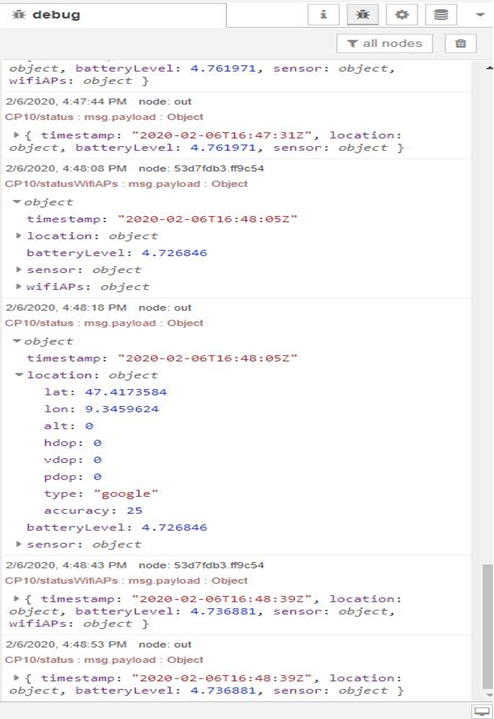
\includegraphics[width=\linewidth]{Chapters/Figures/cp10.png}}%
    }
  \caption{Model Debug Output}
  \label{fig:node_red_debug}
\end{figure}



\begin{figure}[htbp]
  \centering
    \scalebox{0.65}{
    {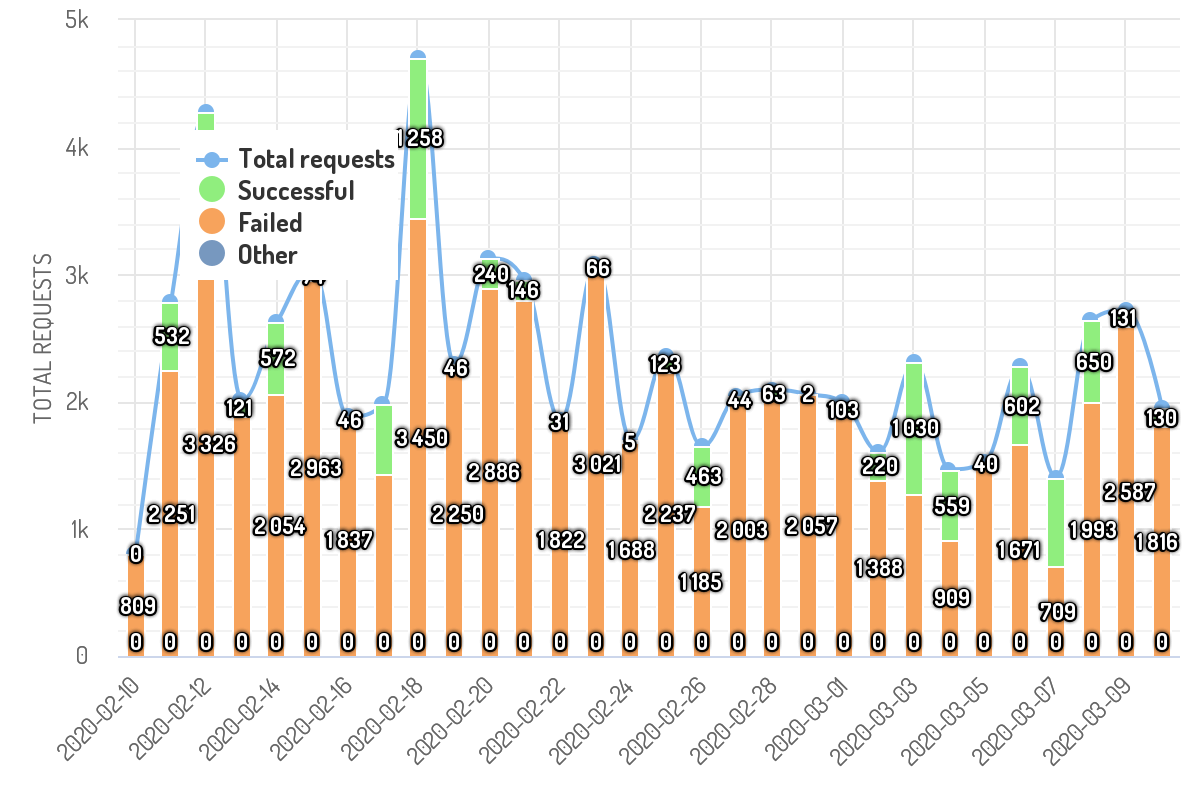
\includegraphics[width=\linewidth]{Chapters/Figures/opencell.png}}%
    }
  \caption{OpenCell ID}
  \label{fig:OpennCellID_chart}
\end{figure}




From the data  in the chart~\ref{fig:OpennCellID_chart}, referent to OpenCellID API is possible to conclude that over 50000 calls were made, meaning that the system has often used the WiFi data, and from the data of the same chart is possible to observe that the result of the location failed several times, that is the reason  why it was important to have 3 APIs, has location sources.

To conclude the system was able to dynamically choose the best location, from the information received. Unfortunately due to the Covid-19 pandemic, the trials with elderly people stopped, which means that the validation for the second stage was not done within real-life trials, being only tested by the author as described in the following section~\ref{sec:Other Analysis}.

%ter uma tabela 3 casos de uso radar com 4 niveis
% subsection Work Scenario (end)



%%%%%%%%%%%%%%%%%%%%%  End use case 3  %%%%%%%%%%%%%%%%%%%%%%%%%%%%%%%%%%




\newpage
%############### Start Other Analysis########
\section{Other Analysis}
\label{sec:Other Analysis}

In this section, will be the other analysis  need for the implementation of the  second functional stage, which is the Advanced. This section will comprise the communication resilience analysis and the power management analysis.


%############### Start Communication Resilience ########
\subsection{Communication Resilience}
\label{sec:Comunication_Resilience}

In this analysis, the author performed tests for communication resilience. These tests were done to test the communication resilience that was first introduced in figure~\ref{fig:Connect} from chapter~\ref{cha:Implementation}. The tests were done since they were necessary for implementing the second functional stage.

These tests were conducted to the two different methods: LoRa and NB-IoT. To test the communication resilience, the communication fallback capabilities were tested. If the device loses the NB-IoT link, it should fall back to using the LoRa stack.
In case the communication network changes, then the Adaptive Geolocation Solver service should be able to handle the data transition and continue the processing of information. It should also be possible to force the change of the communication technology based on the energy efficiency settings.



The work done for the communication resilience in the device side was not done directly by the author, instead was done by Researcher Jorge Calado, and tested in this section.

The first test comprised using the device outdoor, with good NB-IoT signal strength, and then enter an underground parking lot, which was previously tested and had no NB-IoT coverage. A LoRa gateway was set inside the parking lot, to provide LoRa coverage. The test was conducted 5 times, and the device always changed to LoRa after a pre-defined connection time-out of the NB-IoT.

With this result, in the system side was possible to observe that with the change of communication, and the type of the received message, the system could return the same output.

The second test consisted in sending a downlink message in a JSON format, to the device with the communication technology and a boolean value, such as ‘\{”ltenb“: “False”, “lora“: “True”\}’. 

On the device side, the response was similar to the previous test. The device received and decoded the JSON information and started the connection to the LoRa network. If the LoRa connection was unsuccessful, the device reboots and starts transmitting again with NB-IoT.

%############### End Communication Resilience ########
%############### Start power management ########

\newpage
\subsection{Power Management}
\label{subsec:power_management}

For the purpose of getting the results for power consumption, need in the implementation of the Advanced functional stage. An analysis with several tests was conducted to the different communication  and location methods. These tests consisted of logging information from the device, with the aim to discover the battery duration, current and power, to perform  more efficient power management. From the device manufacturer is possible to observe the next figure~\ref{fig:PowerTableAll}, where some values are already provided. All of the tests were conducted in the same fix place, at a  stationary speed, with the same 2 FiPy and two LiPo batteries with 3.7V and 800mAh, the results are the average from 4 tests.

\begin{figure}[htbp]
  \centering
  
    {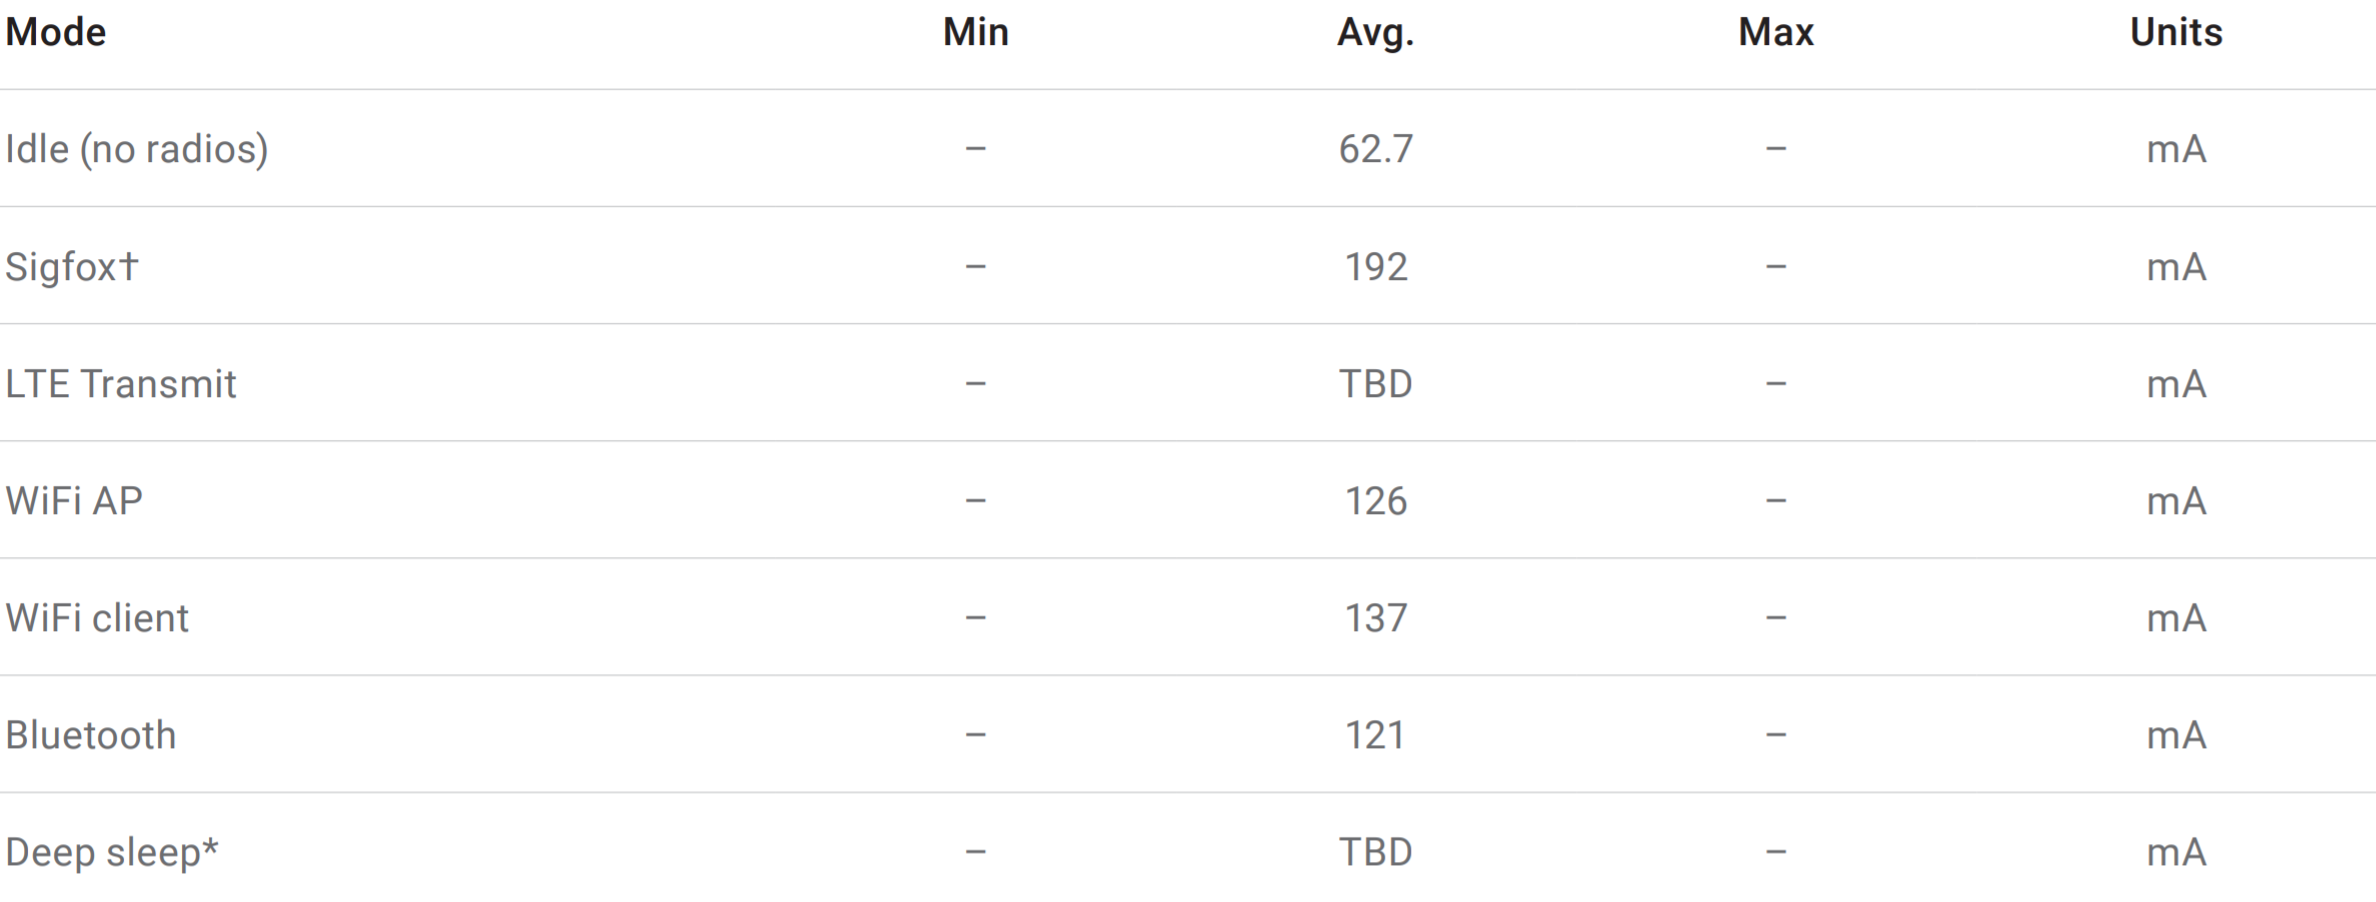
\includegraphics[width=0.93\linewidth]{Chapters/Figures/power1.PNG}}%
 
  \caption{Power Table Fipy~\cite{Microcontroller2017}}
  \label{fig:PowerTableAll}
\end{figure}


\subsubsection{LoRa}
\label{subsec:LoRa}

The first communication method studied was LoRa. To prepare this test was used the two FiPys and after letting the batteries charge for 3 hours with a 2.1A charger connect to devices. The first test was started, using only communication, the Fipy was combined with a pysense (without GNSS and Accelerometer)  shield, and the initial battery was around 4.1V and the end battery as expected was 3.3V. The next test was using the communication but reading one accelerometer sensor, and getting the GPS location, the only difference here was the use of pytrack instead of pysense. The result for the battery duration is lower as expected, for the last test was introduced also the WiFi scan for nearby Access points. The data for all of the tests is in the next table~\ref{tab:LoRa_Power} each test was considered an Operation mode. 

\begin{table}[htbp]
\centering
\begin{tabular}{@{}cclclcl@{}}
\toprule
\multicolumn{1}{l}{} & \multicolumn{2}{c}{\begin{tabular}[c]{@{}c@{}}Communication\\ Only\end{tabular}} & \multicolumn{2}{c}{\begin{tabular}[c]{@{}c@{}}Communication\\ GNSS, Sensor\end{tabular}} & \multicolumn{2}{l}{\begin{tabular}[c]{@{}l@{}}Communication\\ GNSS, Sensor,\\ Scan WiFi\end{tabular}} \\ \midrule
\begin{tabular}[c]{@{}c@{}}Battery  Duration\end{tabular} & \multicolumn{2}{c}{12h} & \multicolumn{2}{c}{9h} & \multicolumn{2}{c}{8h 30m} \\
Average Current & \multicolumn{2}{c}{65mA} & \multicolumn{2}{c}{88mA} & \multicolumn{2}{c}{94mA} \\
Average Power & \multicolumn{2}{c}{240mW} & \multicolumn{2}{c}{326mW} & \multicolumn{2}{c}{351mW} \\ \bottomrule
\end{tabular}
\caption{LoRa Power}
\label{tab:LoRa_Power}
\end{table}

The following figure~\ref{fig:LoRaPowerTable}, represents the current results from the manufacturer, which gives the baseline for the above-mentioned tests. LoRa has different spreading factors the configurations used in this test were the same used in the LoRa section of~\nameref{subsec:laboratory}, that were spreading factor 7, bandwidth 125 kHz, TX power 14 dBm, sample time 30 seconds, message size of $110$ bytes plus $20$ bytes when WiFi was used.

\begin{figure}[htbp]
  \centering
  
    {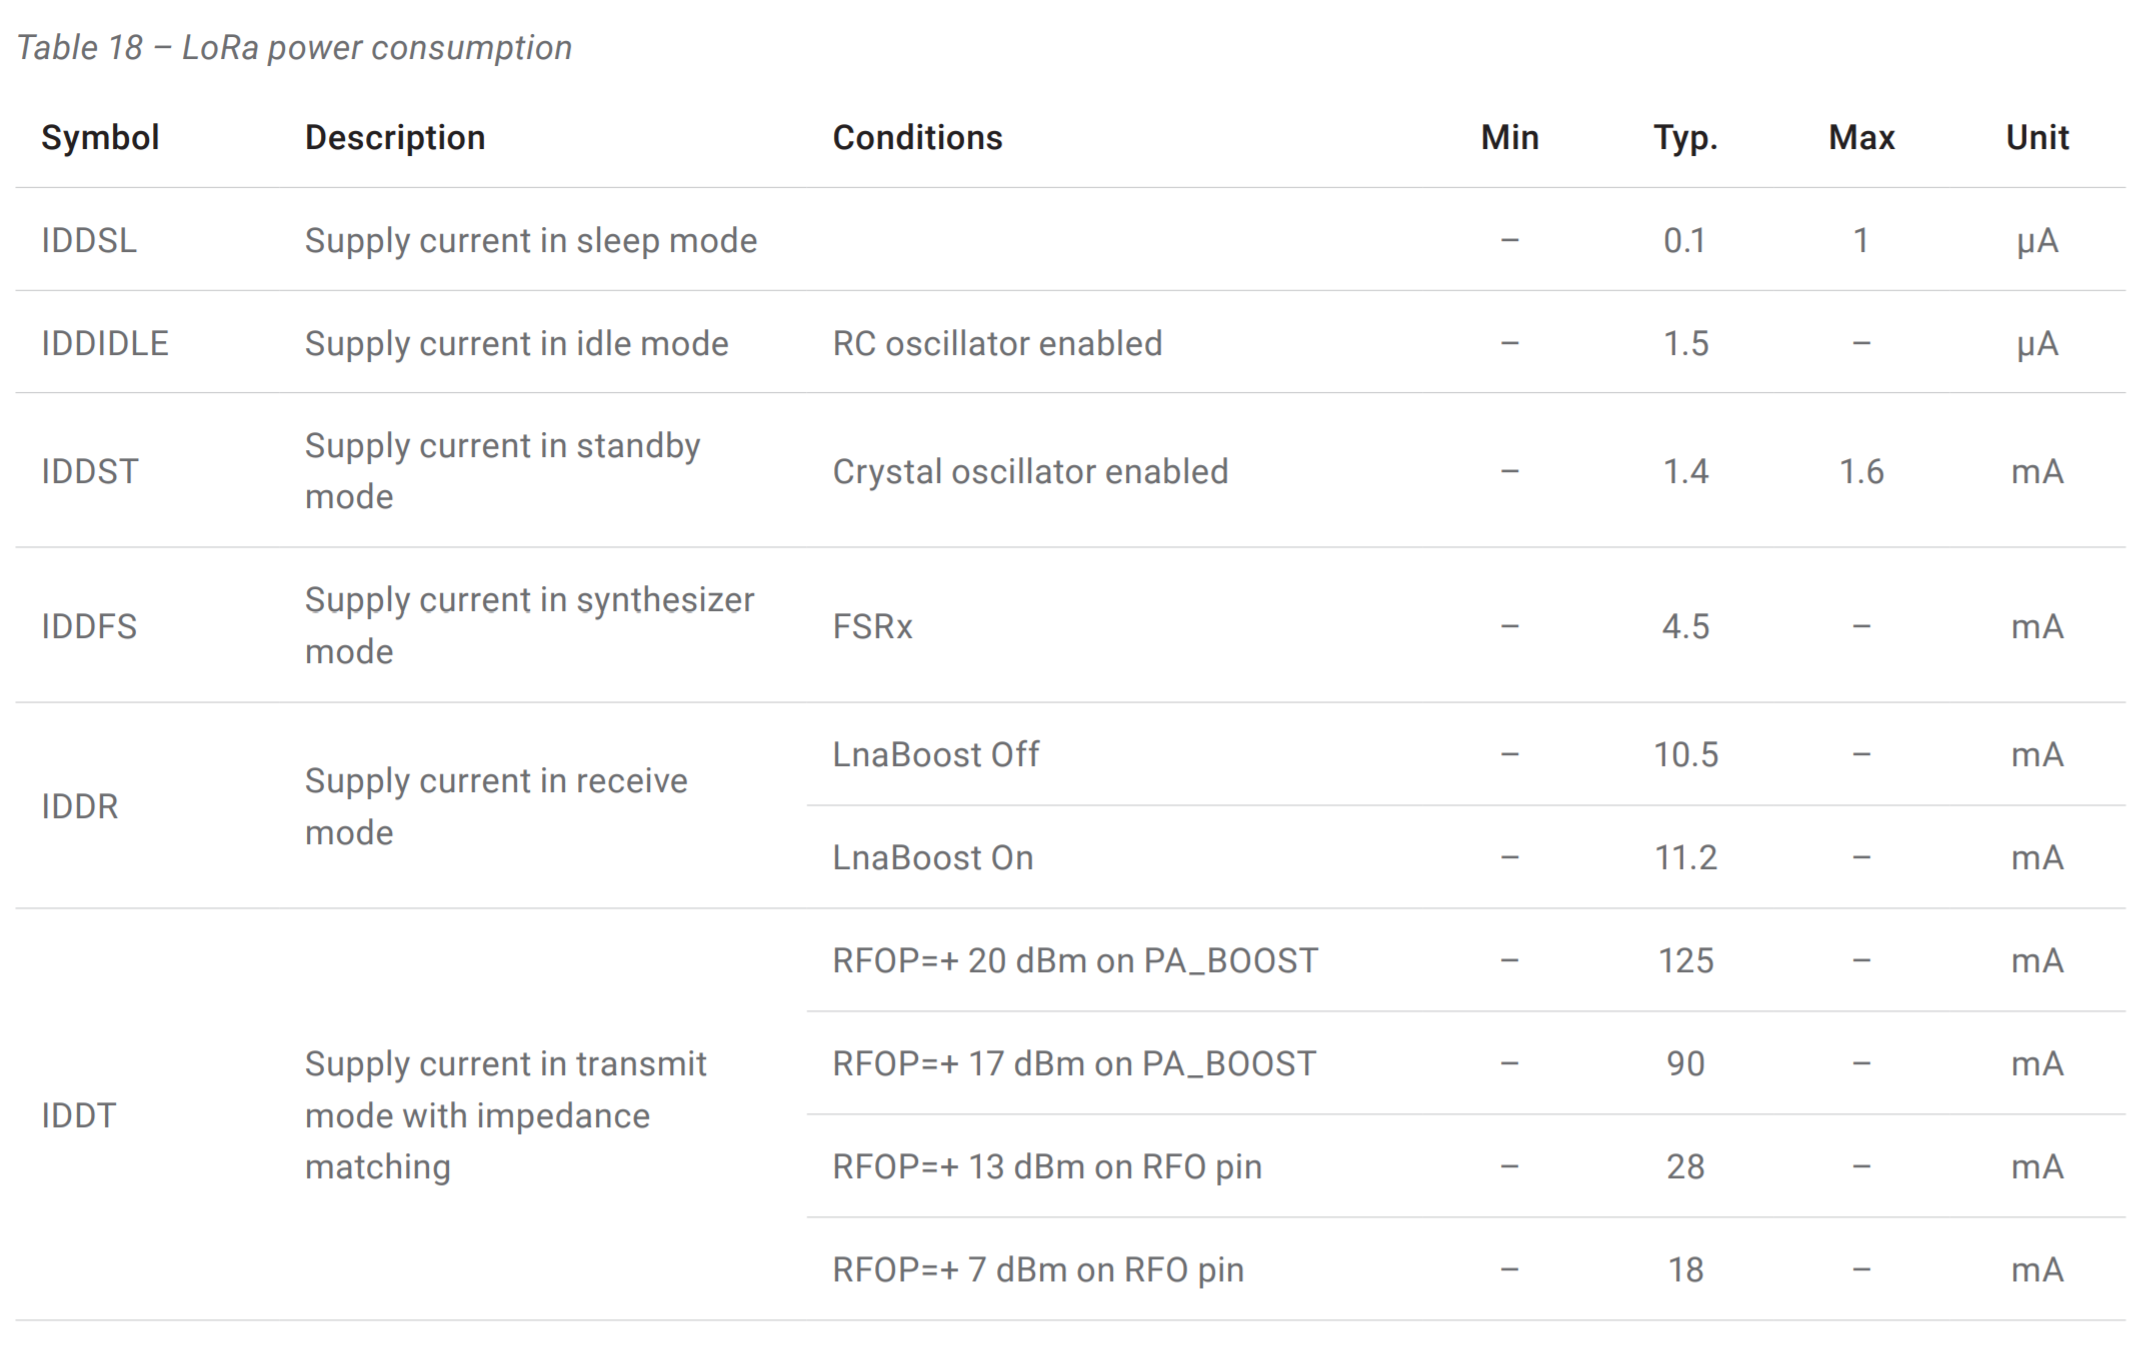
\includegraphics[width=0.91\linewidth]{Chapters/Figures/Lora2.PNG}}%
 
  \caption{LoRa Power Table~\cite{Microcontroller2017}}
  \label{fig:LoRaPowerTable}
\end{figure}

\subsubsection{NB-IoT}
\label{subsec:NB} 

The next communication method used for this test was, NB-IoT. The procedure was the same as above starting by using only communication and then increasing the battery usage with GNSS and accelerometer, ending with all of this plus the scan of WiFi APs. The NB-IoT is expected to have poor performance compared to LoRa, because of the message size of $245$ bytes plus $134$ bytes if WiFi data is used, which is $2.22$ to $2.71$ times higher than LoRa. The results for this method are described in the following table~\ref{tab:NB_Power}.

\begin{table}[htbp]
\centering
    \begin{threeparttable}[!ht]

        \begin{tabular}{@{}cclclcl@{}}
        \toprule
        \multicolumn{1}{l}{} & \multicolumn{2}{c}{\begin{tabular}[c]{@{}c@{}}Communication\\ Only\tnote{*}\end{tabular}} & \multicolumn{2}{c}{\begin{tabular}[c]{@{}c@{}}Communication\\ GNSS, Sensor\end{tabular}} & \multicolumn{2}{l}{\begin{tabular}[c]{@{}l@{}}Communication\\ GNSS, Sensor,\\ Scan WiFi\end{tabular}} \\ \midrule
        \begin{tabular}[c]{@{}c@{}}Battery Duration\end{tabular} & \multicolumn{2}{c}{5h 25m} & \multicolumn{2}{c}{4h 30m} & \multicolumn{2}{c}{4h} \\
        Average Current & \multicolumn{2}{c}{148mA} & \multicolumn{2}{c}{185mA} & \multicolumn{2}{c}{208mA} \\
        Average Power & \multicolumn{2}{c}{548mW} & \multicolumn{2}{c}{685mW} & \multicolumn{2}{c}{770mW} \\ \bottomrule
        \end{tabular}
            
        \begin{tablenotes}
        \item[*] Test not done with final code.
        \end{tablenotes}
    \caption{NB-IoT Power}
    \label{tab:NB_Power}
    \end{threeparttable}
\end{table}

\subsubsection{WiFi}
\label{subsec:WiFi}

The last communication used for these tests was WiFi, this method is expected to have the worst battery performance, but at the same time is the one with higher transfer speeds, meaning the airtime for the same amount of data is lower, so in right circumstances could perform better than the previous two, this was the objective of the test. WiFi could not be used as viable options in the final code due to the short-range, and the need for authentication. Surprisingly, the results for the tests concluded that WiFi had better battery duration that NB-IoT. The reader should be inform that these tests were not done with the final code. They were only with hard-coded values, meaning they do not proof that WiFi is better than NB-IoT, and will not be present in the next section for comparison. These values are expressed in the next table~\ref{tab:WiFi_Power}.\newline
\begin{table}[htbp]
\centering
\begin{threeparttable}[!ht]

    \begin{tabular}{@{}cclclcl@{}}
    \toprule
    \multicolumn{1}{l}{} & \multicolumn{2}{c}{\begin{tabular}[c]{@{}c@{}}Communication\\ Only\tnote{*}\end{tabular}} & \multicolumn{2}{c}{\begin{tabular}[c]{@{}c@{}}Communication\\ GNSS, Sensor\tnote{*}\end{tabular}} & \multicolumn{2}{l}{\begin{tabular}[c]{@{}l@{}}Communication\\ GNSS, Sensor,\\ Scan WiFi\tnote{*}\end{tabular}} \\ \midrule
    \begin{tabular}[c]{@{}c@{}}Battery  Duration\end{tabular} & \multicolumn{2}{c}{5h 40m} & \multicolumn{2}{c}{5h 10m} & \multicolumn{2}{c}{4h 35m} \\
    Average Current & \multicolumn{2}{c}{141mA} & \multicolumn{2}{c}{155mA} & \multicolumn{2}{c}{175mA} \\
    Average Power & \multicolumn{2}{c}{522mW} & \multicolumn{2}{c}{574mW} & \multicolumn{2}{c}{648mW} \\ \bottomrule
    \end{tabular}
    
    \begin{tablenotes}
    \item[*] Test not done with final code.
    \end{tablenotes}
   \caption{WiFi Power}
\label{tab:WiFi_Power}
\end{threeparttable}
\end{table}








\subsubsection{Power Comparison}
\label{subsec:Power_Comparison}
To close this analysis, a comparison with different communications methods, can be observed in the next table~\ref{tab:Battery Duration}. This table combines all of the data from the previous, making easier to compare the different methods, should always be taking into consideration the conditions for the different tests. As expected LoRa had the best battery duration, followed by NB-IoT and WiFi had the worst battery duration. 
\newline


\begin{table}[htbp]
\centering
    \begin{threeparttable}[!ht]

        \begin{tabular}{@{}lccc@{}}
        \toprule
         & NB-IoT & LoRa   \\ \midrule
        1- Communication only & 5h 30m\tnote{*} & 12h &  \\
        \begin{tabular}[c]{@{}l@{}}2- Communication \\ GPS, Sensor\end{tabular} & 4h 30m & 9h   \\
        \begin{tabular}[c]{@{}l@{}}3-Communication\\ GPS, Sensor, Scan WiFi\end{tabular} & 4h & 8h 30m  \\ \bottomrule
        \end{tabular}
            
        \begin{tablenotes}
        \item[*] Test not done with final code.
        \end{tablenotes}
    \caption{Battery Duration}
    \label{tab:Battery Duration}
    \end{threeparttable}
\end{table}


% ########################## End Power Management
% ######################### End other Analysis

% ####################### Start Results Comparison
\newpage
\section{Results Comparison}
\label{sec:geocompare}


In this section, the objective is to clarify and compare the different geolocation techniques from the three use cases. The first geolocation tested was BLE, the optimal scenario for this will be indoor, short-range location, for example, to know if a person is in some room, or in a building to know in which floor the person is at. The second one in the study was the GNSS. This is the classic for solving location problems, and the best fit would be outdoor in a rural environment, but it will also work in an urban environment. The third one is WiFi and the best scenario for this assisted location will be urban outdoor, where the accuracy for the results can be close to GNSS, but it is also a viable options for a use case where the person is in a constant transition from indoor to outdoor environments. The last one, is the analyse of the LoRa Metadata, where the optimal scenario for this assisted location will be urban or rural outdoor, but can also work Indoor. The best fit for this technique is essentially when none of the others is available or the remaining battery is to low.

The next figure~\ref{fig:radar1} uses a radar diagram, to provide a visual and easier interpretation, of the obtained results, the axis value 1 correspond to Poor, . It is used for  comparing the different geolocation techniques with each other. In the figure, the vertical axis values from 1 to 4 correspond to the following levels Poor, Fair, Good, Excellent.
\begin{figure}[htbp]
  \centering
  
    {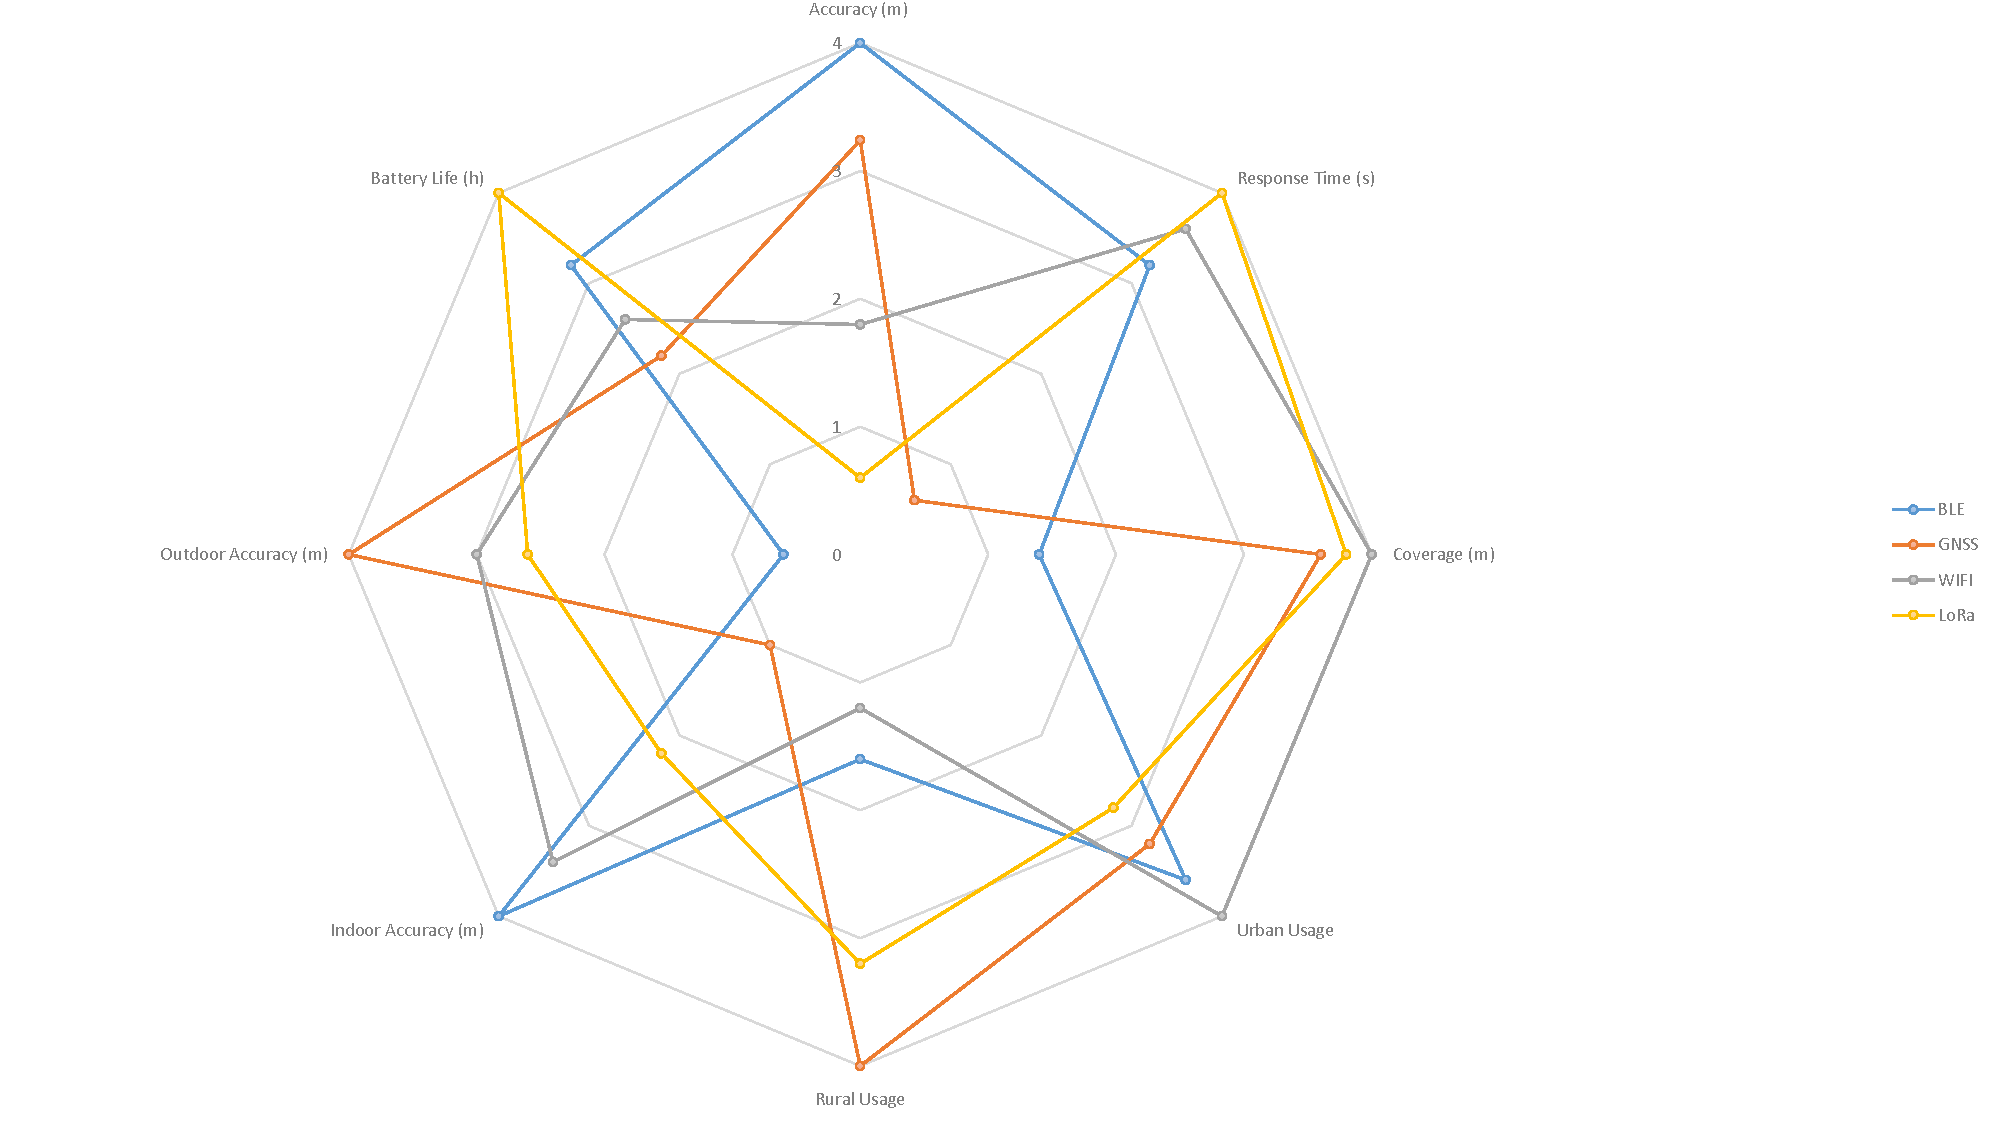
\includegraphics[width=\linewidth]{Chapters/Figures/radarfinal3.pdf}}%
 
  \caption{Geolocation Results Comparison}
  \label{fig:radar1}
\end{figure}

From the previous figure, the next graphic~\ref{fig:radarline} was done. In this graphic is possible to observe the best technique to use in every different situation. It is possible to observe that there is not a technique better than the others in every situation. In the red arrow represented in the graphic is explained the situation where WIFI is the best suit for a mixed indoor/outdoor accuracy. Although it is not the best neither Indoor (BLE) nor Outdoor (GNSS). With   close observation of this graphic, can be concluded that the best solution is a profile-based decision system, capable of choosing at any moment the best technique to use.

\begin{figure}[htbp]
  \centering
  
    {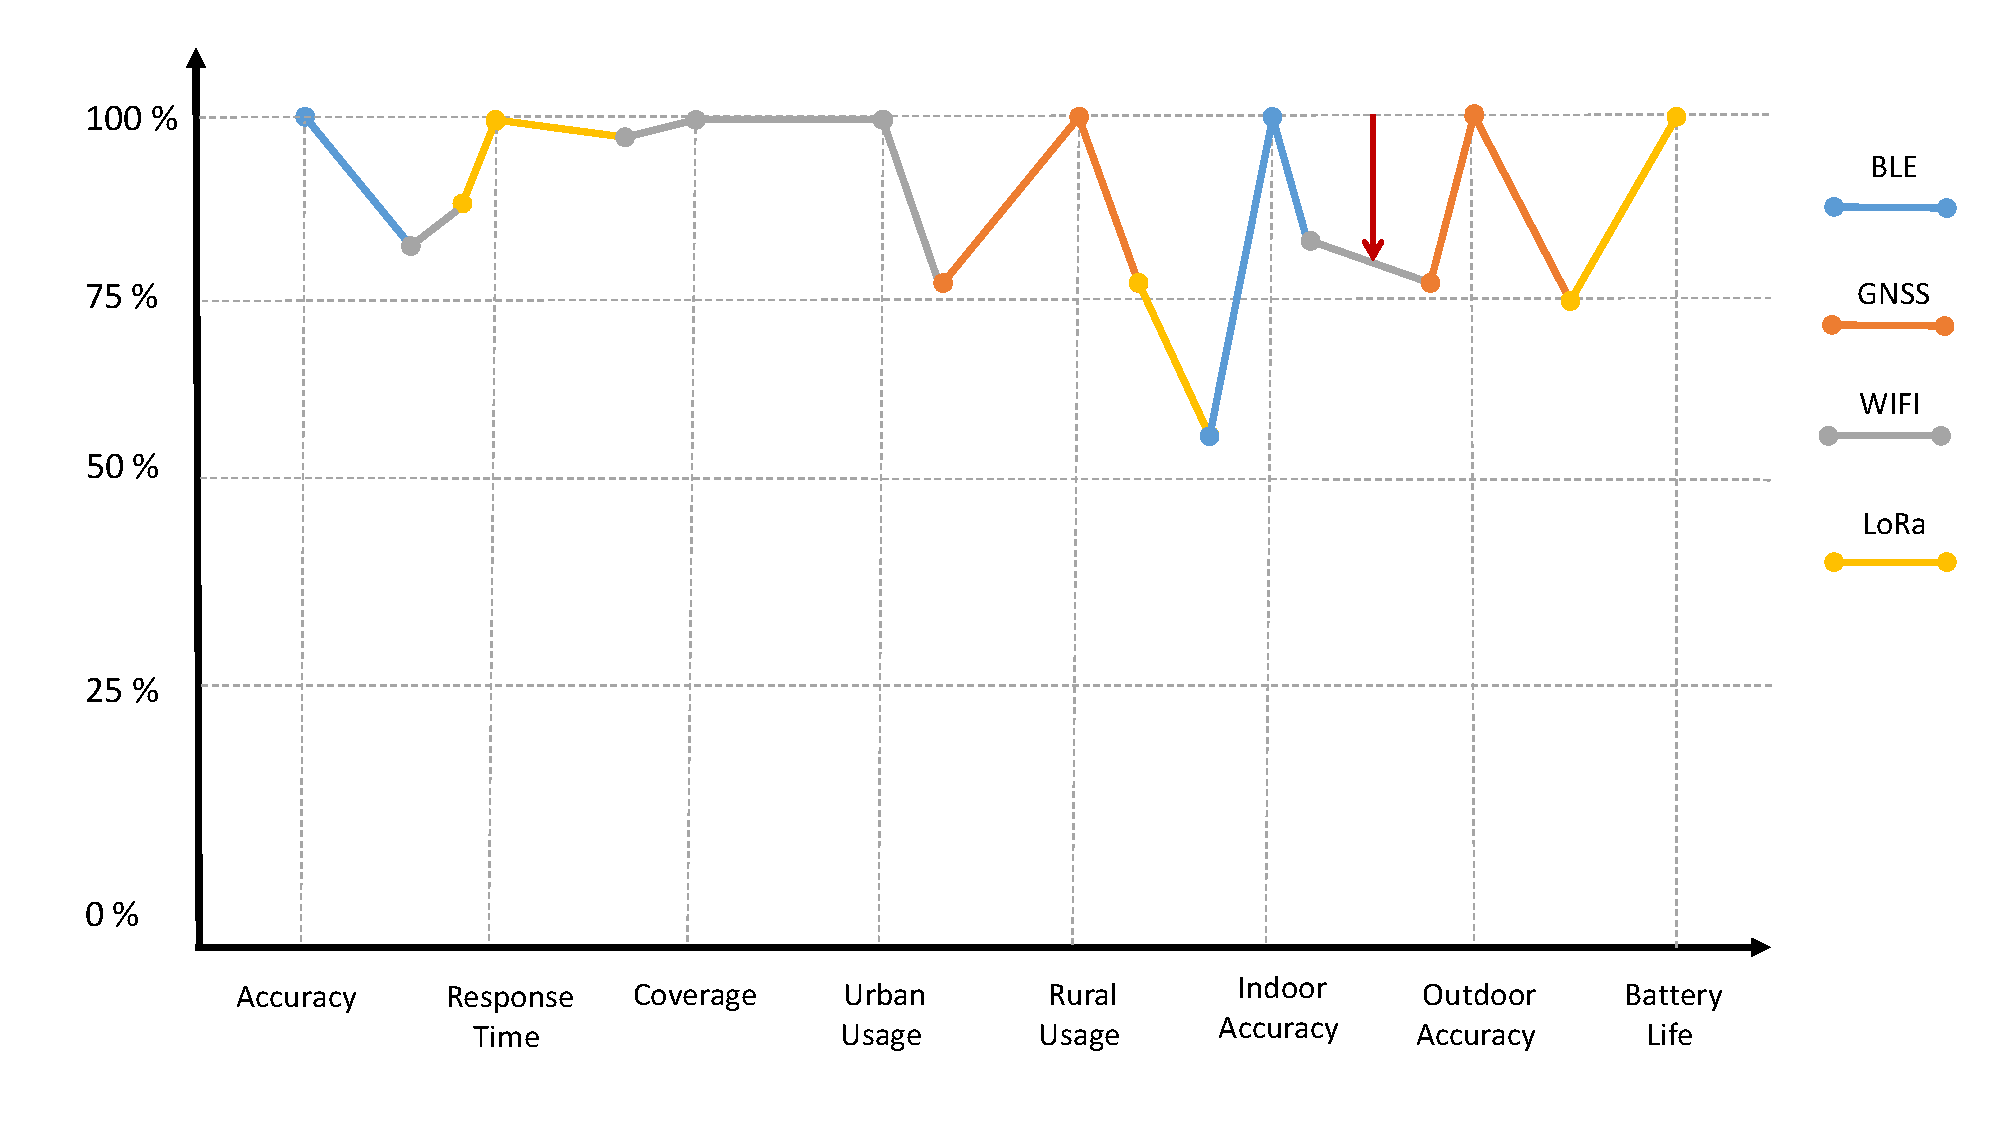
\includegraphics[width=0.9\linewidth]{Chapters/Figures/radarline.pdf}}%
 
  \caption{Geolocation Results Comparison line}
  \label{fig:radarline}
\end{figure}

%################## End Results Comparison ################


%################# Start Discussion

\section{Discussion}
\label{sec:Discussion}

One initial objective was to  determine what kind of impact had LPWAN enabled solutions in wearable devices, in particular those focused on people with dementia.\newline 
It was hypothesized that people dealing with dementia would benefit from LPWAN enabled solutions. Since they would help in perform the location of the person, while saving battery, reducing the overall cost, and comply with the technical constraints of wearable devices. Having also the possibility to dynamically choose, the best location available in that moment. 

The results accuracy match those mentioned in previous studies of geolocation technologies and techniques, and that are represented in~\nameref{sec:related_work}.\newline 
There are several possible explanations for the results, since the used hardware, to the environmental conditions, for example, if the tests were taken outdoor in an urban or rural place. 

With these results, in the system  was possible to observe that with the change of communication, and the type of received message the system was capable of returning the same output, and perform the adaptive geolocation.\newline 
These results provide support for the hypothesis that LPWAN can be used for the locations o people with dementia, while accounting for the constraints of wearable IoT devices.



%!!!!!(Esta secção poderá ser combinada na conclusão) !!!!


%################# End Discussion




%################# End Results





















